\documentclass[a4paper,12pt,dvipdfmx]{jreport}

\usepackage[dvipdfmx]{graphicx}
\usepackage{comment}
\usepackage{cite} 
\usepackage{url}
\usepackage{ascmac}
\usepackage{amsmath}
\usepackage{algorithm, algpseudocode}
\algnewcommand\algorithmicforeach{\textbf{for each}}
\algdef{S}[FOR]{ForEach}[1]{\algorithmicforeach\ #1\ \algorithmicdo}
\renewcommand{\algorithmicrequire}{\textbf{Input:}}
\renewcommand{\algorithmicensure}{\textbf{Output:}}

\usepackage{siunitx}
\usepackage{enumerate}

%%% sty
\usepackage{sty/master_thesis}
\usepackage[a4paper,textheight=21.7cm,top=3cm,left=2cm,right=2cm,headheight=15pt]{geometry}

% しおり(bookmark)つきのpdf文書作成
\usepackage[dvipdfmx,%
 bookmarks=true,%
 bookmarksnumbered=true,%
 colorlinks=false,
 pdfborder={0 0 0}]{hyperref}
\AtBeginDvi{\special{pdf:tounicode EUC-UCS2}}

% ヘッダに章の名前を表示
\usepackage{fancyhdr}
\pagestyle{fancy}
\renewcommand{\chaptermark}[1]{\markboth{\small 第\ \thechapter\ 章 #1}{}}
\rhead{\leftmark}
\lhead{}
\makeatother

\年度{2024}
\題目{ビットごとのT-depthを考慮した\\ MCTゲートの分解手法}
\指導教官{山下 茂}
\学籍番号{6611230046-6}
\氏名{廣野 航輝}
\コース{計算機科学コース} %計算機科学コース or 人間情報科学コース

\begin{document}
\baselineskip 1.9zw
\maketitle


\newpage
\thispagestyle{empty}
\pagenumbering{roman}
\setcounter{page}{1}
\chapter*{内容梗概}
量子回路設計において,T-depthを削減することが非常に重要である.
T-depthを削減するようなMultiple Controlled Toffoli(MCT)ゲートの分解手法が研究されている.
既存のMCTゲートの分解では,分解を工夫することで,MCTゲートのT-depthを削減している.
複数のMCTゲートを分解する場合,ビットごとのT-depthに差が生じる.
既存のMCTゲートの分解手法では,ビットごとのT-depthを考慮していないため,
既存のMCTゲートの分解手法は最適でない可能性がある.
\par
本論文では,ビットごとのT-depthを考慮して,
MCTゲートの分解を行うことで,
T-depthを削減する手法を提案する.
提案手法では,T-depthの小さいビットを優先して使用し,
MCTゲートを分解することでT-depthを削減する.
また,後続のゲートを考慮して,
MCTゲートの分解を決定することで回路全体のT-depthを削減する.
提案手法を用いることで,
既存手法より,\rout{T-depthを平均17.1%削減できる}ことを確認した.
\begin{comment}
\begin{itemize}
\item 12/20 ver0 目次案作成
\item 12/23 ver1 第一章作成
\item 12/26 ver2 同期チェックの結果を反映:\rout{赤色で修正}
\item 12/27 一章,先生のコメントを反映:\gout{緑色で修正}
\item 12/28 chap2\_ver0:第二章作成
\item 12/30 chap2\_ver1:同期チェックを反映:\gout{緑色で修正}
\item 12/31 chap2\_ver2:先生のコメントを反映:\bout{青色で修正}
\item 1/5 chap3\_ver0:第三章作成
\item 1/7 chap3\_ver1:同期チェックを反映:\bout{青色で修正}
\item 1/13 chap3\_ver2:先生のコメントを反映:\mout{赤紫色で修正}
\item 1/14 chap3:先生のコメントを反映:\rout{赤色で修正}
\item 1/17 chap4\_ver0:第4章作成
\item 1/18 chap4\_ver1:同期チェックを反映:\rout{赤色で修正}
\item 1/21 chap4\_ver2:先生のコメントを反映:\bout{青色で修正・追加}
\item 1/22 chap5\_ver0:第5章作成
\item 1/22 chap5\_ver1:同期チェックを反映:\rout{赤色で修正}
\item 1/23 chap5:先生のコメントを反映:\bout{青色で修正}
\item 1/23 chap6\_ver0:第6章作成
\item 1/23 chap6\_ver1:同期チェックで特に指摘なし
\item 1/24 chap6:先生のコメントを反映:\rout{赤色で修正}
\end{itemize}
\end{comment}

\newpage
\tableofcontents
\listoffigures
\listoftables

\newpage
\pagenumbering{arabic}
\chapter{はじめに}

%\begin{itemize}
  %\item どのような分野の研究か,その背景について説明する.
  %  \begin{itemize}
 %     \item 量子計算を実現する量子回路は与えられた論理関数ごとに設計する必要がある.
  %    \item 複数のMCTゲートを組み合わせることで,任意の論理関数を設計できる.
   %   \item 実際の量子コンピュータでMCTゲートを実行するには,Clifford+Tと呼ばれるゲート群に分解する必要がある.
   %   \item 量子回路中の同時に実行できないTゲートの段数をT-depthと呼ぶ.
   %   \item Tゲートは実行時間が他のClifford+Tのゲートと比べ長いため,T-depthはコストの指標として用いられる.
   %   \item T-depthを削減するような量子回路の設計手法が求められている.
   % \end{itemize}
    量子計算機は,量子力学における量子の重ね合わせ状態を利用して計算する\cite{nielsen2010quantum}.
    量子計算機には従来の計算機と比較して高速に計算できる量子アルゴリズムが存在する.
    代表的な量子アルゴリズムとして,素因数分解を高速に解くことができるShorのアルゴリズム\cite{shor1999polynomial}
    や整理されていないデータベースを高速に探索できるGroverのアルゴリズム\cite{grover1996fast}などが挙げられる.
    これらの量子アルゴリズムの発見により,量子計算機の研究が盛んに行われるようになった.
    また,物理的な限界により,集積回路の性能向上は困難になると考えられている\cite{2015Inte81:online}.
    このため,従来の計算方式と異なる計算方式を持つ量子計算機が注目されている.
    \par
    一般的な量子アルゴリズムには論理関数を計算する部分が存在する\cite{yamashita2008ddmf}.
    この論理関数を計算する量子回路は与えられた論理関数ごとに設計する必要がある.
    量子回路設計では,Multiple Controlled Toffoli(MCT)ゲート\cite{barenco1995elementary}を用いて論理関数を設計する.
    MCTゲートの演算を実現するには,\rout{Clifford+Tと呼ばれるゲート群に分解する必要がある}\cite{zhou2000methodology}.
    このClifford+Tのゲート群の中に,Tゲートと呼ばれるゲートがある.
    Tゲートの操作時間は他のClifford+Tのゲートと\gout{比較して非常に}長い\cite{fowler2009high}.
    このため,量子回路中の\rout{同時に実行できないTゲートの段数であるT-depthを削減すること}が量子回路設計において重要な課題である\cite{amy2013meet,miller2014mapping,selinger2013quantum}.
    T-depthを削減するような,MCTゲートの分解手法が研究されている\cite{abdessaied2016technology,niemann2019t,baker2019decomposing}.

  %\item その分野の従来の研究状況について説明
  %\begin{itemize}
  %  \item MCTゲートの分解を工夫することでT-depthを削減する手法が提案されている.
  %  \item 既存手法では,ビットごとのT-depthの値を均一に考えている
  %\end{itemize}
  %\item そして,何が解決すべき問題(本論文で扱った問題)かを説明.
  %\begin{itemize}
  %  \item 既存手法では,ビットごとのT-depthの値を考慮していない
  %  \item T-dephが大きいビットを先に使用することでT-depthが悪化する場合がある
  %\end{itemize}
  \par
  \gout{複数のMCTゲートを分解するとビットごとのT-depthの値に差が生じるが,
  既存のMCTゲートの分解手法\cite{abdessaied2016technology,niemann2019t,baker2019decomposing}ではその差を考慮していない.}
  このため,既存のMCTゲートの分解手法では,
  複数のMCTゲートを分解する際に,T-depthの値が大きいビットを先に使用することでT-depthが\rout{増加}する場合がある.
  %\item どのようなアイデアで解決したか,キーアイデアを少しだけ披露
  %\begin{itemize}
  %    \item ビットごとのT-depthを計算
  %    \item T-depthが小さいビットを優先的に使用し,MCTゲートを分解
  %    \item ビームサーチを用いて,後のゲートを考慮してMCTゲートを分解
  %\end{itemize}
  \gout{そこで,}本論文では,ビットごとのT-depthの値を考慮し,
  T-depthの小さなビットを優先的に使用することでT-depthを削減する手法を提案する.
  \par
  複数のMCTゲートを分解する場合,貪欲にT-depthの小さなビットを使用すると,回路全体のT-depthが\rout{増加}する場合がある.
  そのため,MCTゲートを分解する際に後続のゲートを考慮する必要がある.
  \gout{そこで,}本論文では,ビームサーチを用いて後続のゲートを考慮し,MCTゲートを分解することでT-depthを削減する手法も提案する.
  %\item どのような(実験)結果が得られたか、アピール(目次案の段階では希望的予測)
   % \begin{itemize}
   %   \item 回路に初期化されていない補助ビットを与えた場合,0で初期化された補助ビットを与えた場合それぞれで実験.
   %   \item すべてのゲートを分解した後の最大のT-depthで比較
   %   \item 平均XX\%,既存手法からT-depthを削減
  %  \end{itemize}
  \par
  提案手法,既存手法\cite{abdessaied2016technology,niemann2019t,baker2019decomposing}を
  ベンチマーク回路\cite{wille2008revlib}に適用し,比較実験を行った.
  比較の指標には,\rout{手法適用後の回路における}最大のT-depthを用いた.
  提案手法は既存手法を適用した場合に比べ,最大のT-depthを平均\rout{17.1}%\rout{削減することが確認された.}
  % すべての実験結果の平均の削減率.
  %\item 章構成
  %  \begin{itemize}
  %    \item 本論文は6章で構成されている.
  %    \item 第2章で量子回路と量子ゲートの基礎知識について述べる.
  %    \item 第3章では,既存のMCTゲートの分解手法について述べる.
  %    \item 第4章では本論文の提案手法について述べる.
  %    \item 第5章では提案手法の評価方法と実験結果,考察について述べる.
  %    \item 第6章では本論文のまとめと,今後の課題について述べる.
  %  \end{itemize}
  \par
  本論文は6章から構成される.
  第2章では量子回路,量子ゲートとビームサーチの基礎的な知識について述べる.
  第3章では,既存のT-depthを削減するようなMCTゲートの分解手法について述べる.
  第4章では,ビットごとのT-depthを考慮したMCTゲートの分解手法について説明する.
  第5章では,提案手法の評価方法,実験結果と考察について述べる.
  第6章では,本研究のまとめと今後の課題について述べる.
%\end{itemize}
\chapter{基礎知識}
本章では,量子回路,量子ゲートとビームサーチの基礎知識について説明する.
\section{量子回路}
量子回路は,量子計算\cite{deutsch1985quantum}を
量子ゲートと量子ビットを用いて表したものである.
量子ビットと量子ゲートは従来の計算機におけるビットと論理ゲートに相当する.
量子ゲートは従来の論理ゲートと同様に入力と出力を持つ.
複数の量子ゲートを組み合わせることで目的の演算を実現することができる.
量子回路は常に可逆性を持たなければならないという,論理回路とは異なる性質を持つ.
つまり,量子回路は出力から入力が一意に求めることができなければならない.
\par 
\begin{figure}[tbp]
  \centering
  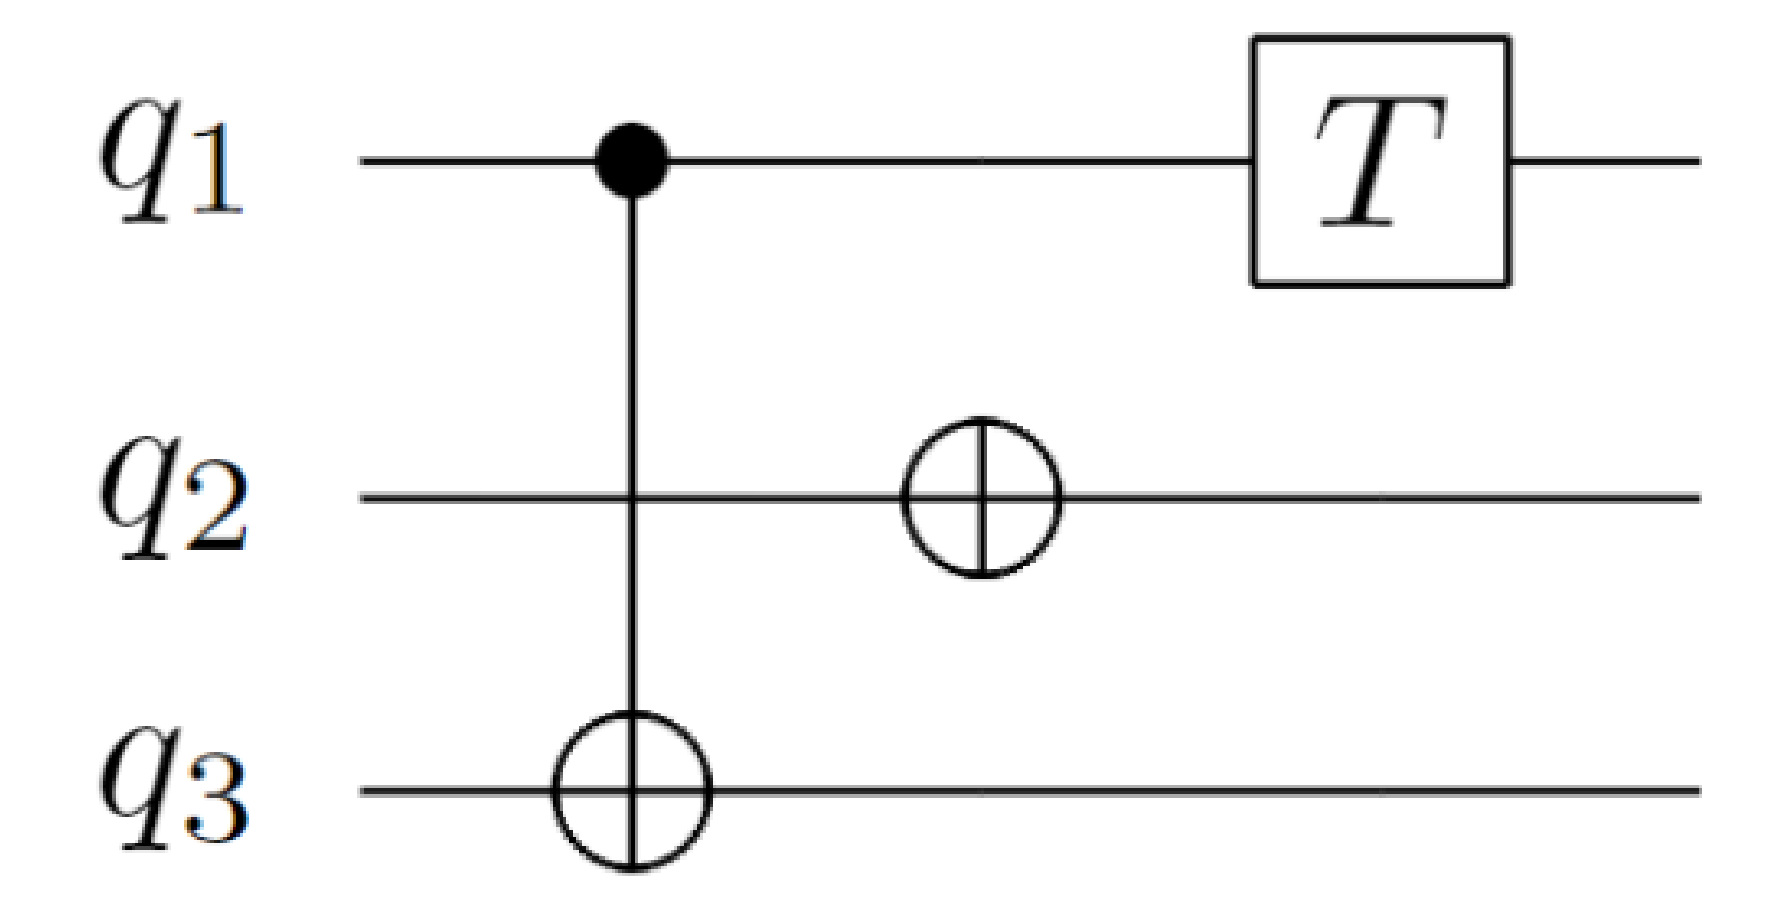
\includegraphics[width=7cm]{img/qcircuit.pdf}
  \caption{量子回路の例}
  \label{qcircuit}
\end{figure}
量子回路の例を図~\ref{qcircuit}に示す.
図~\ref{qcircuit}中の$q_{1}$,$q_{2}$,$q_{3}$というラベル付けされた横線は
量子ビットを表す.
量子ゲートは,図~\ref{qcircuit}のように各ゲートに対応するシンボルで図示される.
量子回路は左側が入力で右側が出力である.
そのため,量子ゲートは左のゲートから順に実行される.
\section{量子ゲート}
量子ゲートは,量子ビットの量子状態を変化させる機能をもつ.
量子ゲートは量子ビットを入力に持ち,コントロールビットとターゲットビット
で構成される.量子ゲートの中にはコントロールビットを持たないものも存在する.
コントロールビットは,量子ゲートをターゲットビットに作用させるかどうかを判定する
量子ビットである.
コントロールビットの値が1のとき,量子ゲートをターゲットビットに作用させる.
一方,ターゲットビットは,コントロールビットの条件が満たされると,
量子ゲートの演算結果によって状態が変化させられる量子ビットのことである.
\par
量子ゲートにはClifford+T\cite{zhou2000methodology}と呼ばれる
$NOT, CNOT, H, T,T^{\dagger}$ゲートからなるゲート群がある.
\gout{エラー訂正を行いながら所望の計算を行う,フォールトレラントな量子計算の枠組みで,}
演算を行うにはこのClifford+Tのゲート群に量子ゲートを分解する必要がある\cite{boykin2000new}.
\par
\bout{量子ゲートが量子ビットに対して行った操作を元に戻す操作のことを逆変換と呼ぶ.
逆変換を行う量子ゲートは,$\dag$を付けて表すことができる.
例えば,$T$ゲートの逆変換は$T^{\dag}$ゲートである.
$T$ゲートを作用させた後に$T^{\dag}$ゲートを作用させると,
$T$ゲートを作用させる前の状態に戻すことができる.}
\subsection{NOT ゲート}
NOT ゲートは従来の計算機の NOTゲートと同じ機能を持つ.NOT ゲートの例を
図~\ref{not_gate}に示す.NOTゲートは1量子ビットのターゲットビットのみで構成されたゲートである.
NOTゲートはターゲットビットの値が$0$ならば$1$を出力し,$1$ならば$0$を出力する.
\begin{figure}[tbp]
  \centering
  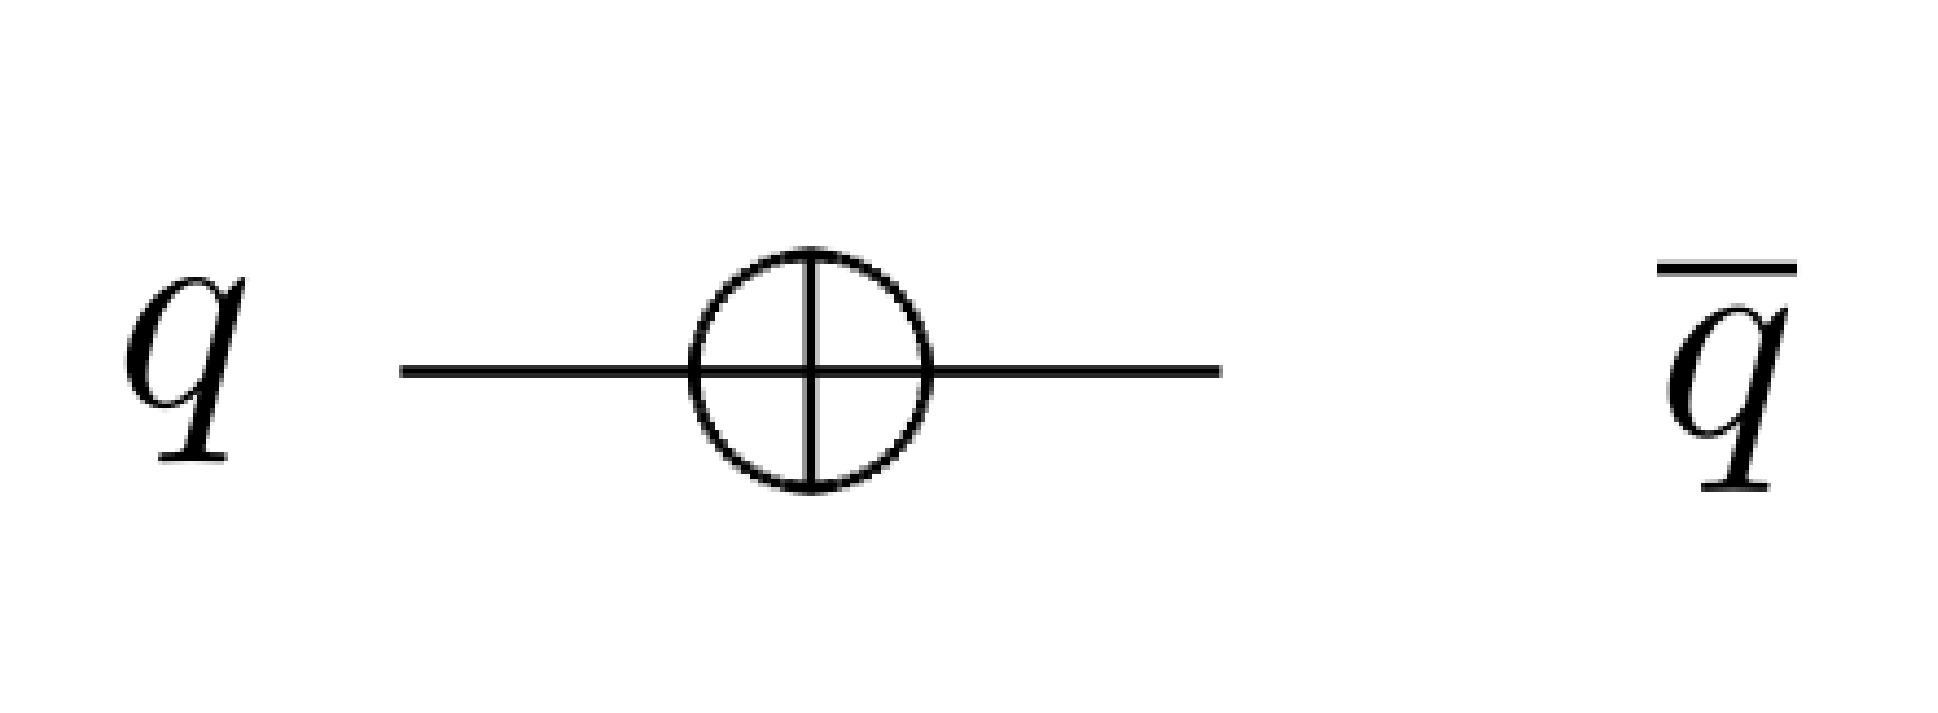
\includegraphics[width=7cm]{img/notgate.pdf}
  \caption{NOTゲート}
  \label{not_gate}
\end{figure}
\subsection{CNOTゲート}
CNOTゲートは1つのコントロールビットと1つのターゲットビットで
構成された量子ゲートである.
CNOTゲートの例を図~\ref{cnot_gate}に示す.
\begin{figure}[tbp]
  \centering
  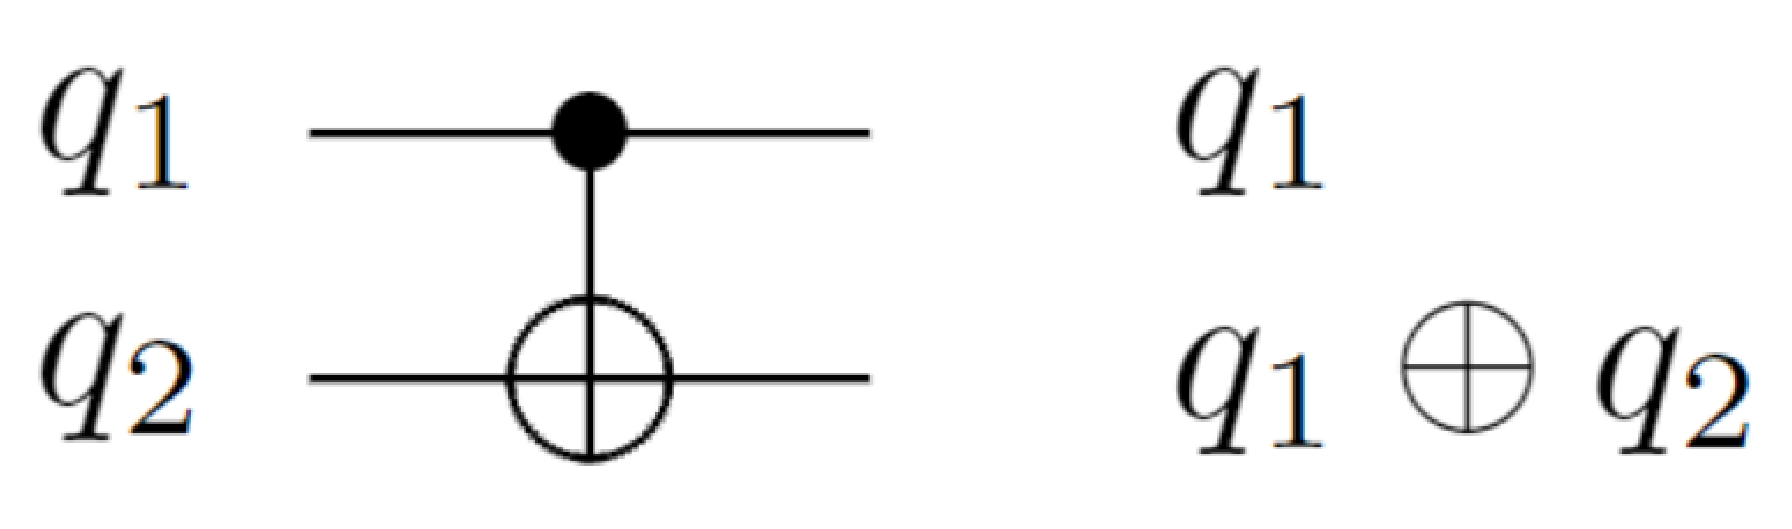
\includegraphics[width=8cm]{img/cnotgate.pdf}
  \caption{CNOT ゲート}
  \label{cnot_gate}
\end{figure}
図~\ref{cnot_gate}中の黒丸●をコントロールビットと呼び,
$\oplus$をターゲットビットと呼ぶ.
CNOTゲートはコントロールビットの値が0のときターゲットビットを変化させず,1のときターゲットビットを反転させる.
コントロールビットの値は変化することはないため,
量子ビット$q_{1}$の値はCNOTゲートを通過しても変化しない.
\subsection{Tゲート}
\bout{$T$ゲートは,作用させる量子ビットの値が1のとき,}
量子状態の位相を$\frac{\pi}{4}$変化させる1量子ビットの量子ゲートである.
\bout{また,$T$ゲートの逆変換を$T^{\dag}$ゲートと呼ぶ.}
\bout{$T^{\dag}$ゲートは$T$ゲートの逆変換であるため,作用させる量子ビットの値が1のとき,
量子状態の位相を$-\frac{\pi}{4}$変化させる.}
$T$ゲート,$T^{\dag}$ゲートの例を図\ref{T_T_dag}に示す.
\begin{figure}[tbp]
  \centering
  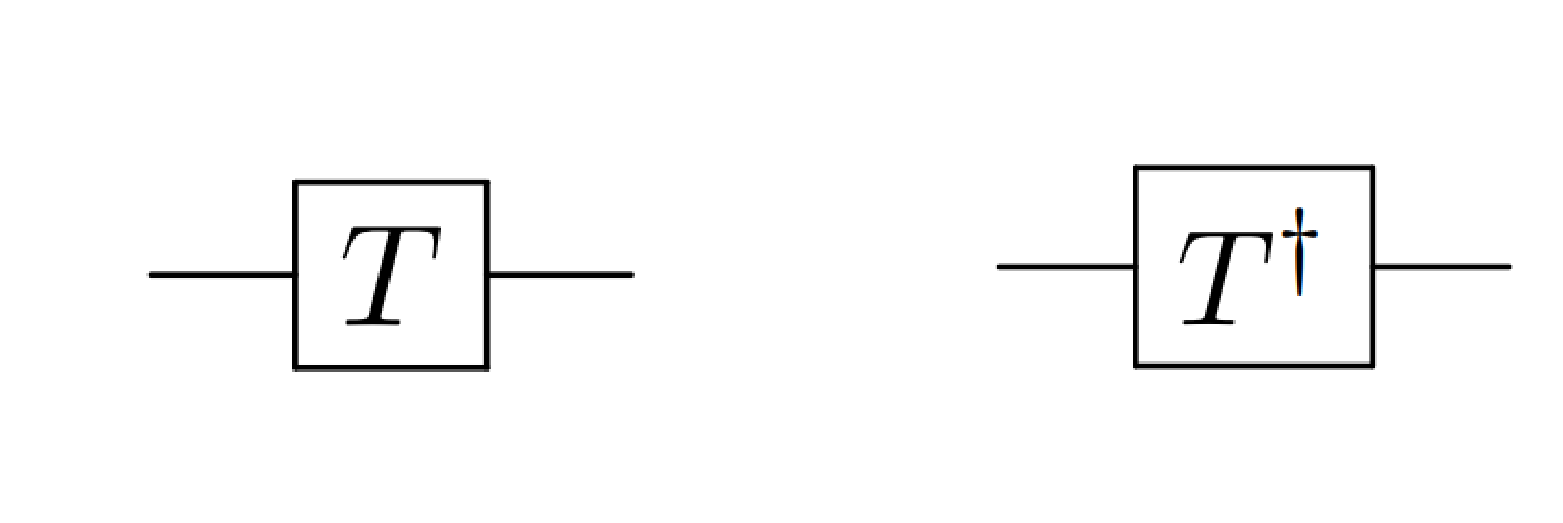
\includegraphics[width=7cm]{img/T_T_dag.pdf}
  \caption{$T$ゲート,$T^{\dag}$ゲート}
  \label{T_T_dag}
\end{figure}
\par
$T$ ゲート,$T^{\dagger}$ゲートの操作時間は他のClifford+Tのゲート群の量子ゲートと比較して非常に長い\cite{fowler2009high}.
そのため,量子回路中の同時に実行できない$T$ゲート,$T^{\dag}$ゲートの段数をT-depth\cite{amy2013meet}と呼び,
T-depthの値を削減することが,量子回路設計の課題とされている.
本論文ではT-depthのみを考慮するため,$T$ゲート,$T^{\dag}$ゲートをまとめて$T$ゲートと呼ぶ.
\subsection{Toffoliゲート}
Toffoliゲートは3量子ビットの量子ゲートである.
Toffoliゲートは,2つのコントロールビットと1つのターゲットビットで構成される.
Toffoliゲートは,すべてのコントロールビットの値が1であるとき,ターゲットビットの値を反転する.
Toffoliゲートの演算を実現するには,Clifford+Tのゲート群に分解する必要がある.
図~\ref{toffoli}にToffoliゲートとその分解例を示す\cite{amy2013meet}.
\par
図~\ref{toffoli}の分解例では,同時に実行できない$T$ゲートが3段現れる.
このため,図~\ref{toffoli}のToffoliゲートのT-depthは3となる.
\begin{figure}[tbp]
  \centering
  \includegraphics[width=11cm]{img/toffoli.pdf}
  \caption{ToffoliゲートとClifford+Tへの分解例\cite{amy2013meet}}
  \label{toffoli}
\end{figure}
\subsection{Multiple Controlled Toffoli(MCT)ゲート}
Toffoliゲートを一般化したものをMultiple Controlled Toffoli(MCT)ゲート\cite{barenco1995elementary}と呼ぶ.
MCTゲートは複数のコントロールビットと1つのターゲットビットで構成される.
MCTゲートはすべてのコントロールビットの値が1のとき,ターゲットビットビットの値を反転する.
\par
MCTゲートもToffoliゲートと同様にClifford+Tのゲート群に分解する必要がある.
コントロールビット数が3個以上の
MCTゲートを分解するには,
補助ビットと呼ばれる値を一時的に保存するビットを使用する必要がある.
ここで使用した補助ビットは,値を復元する必要がある.
\gout{MCTゲートは,}
補助ビットを用いずにClifford+Tに分解できるゲート,
例えばToffoliゲートに,\gout{一度分解される.}
そして,分解したゲートをClifford+Tのゲート群に分解する.
\par
図~\ref{barenco}にコントロールビット数が4個のMCTゲートのToffoliゲートへの分解例を示す.
\begin{figure}[tbp]
  \centering
  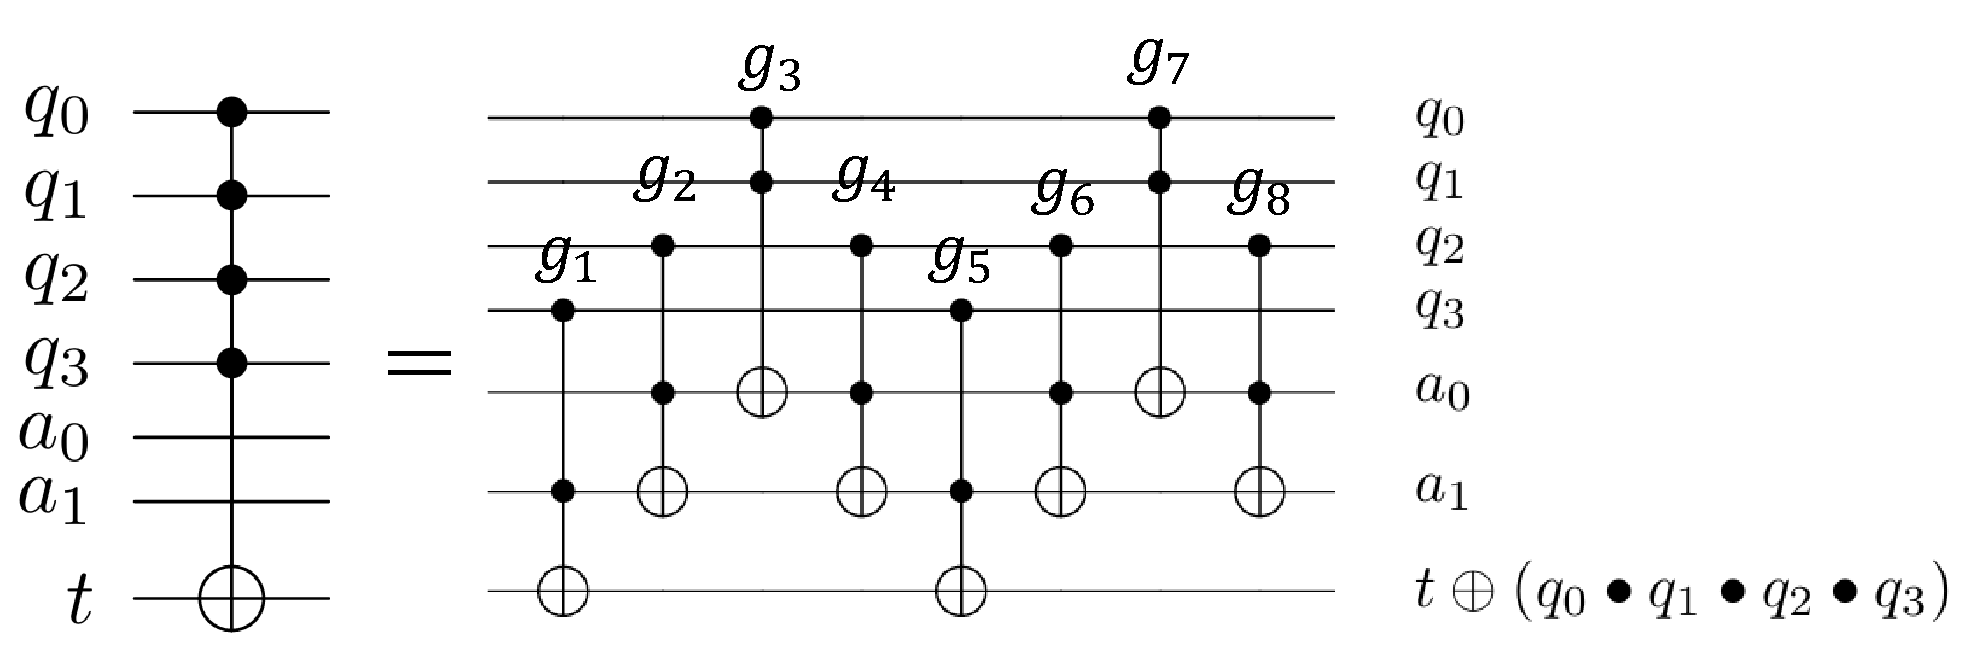
\includegraphics[width=13cm]{img/barenco.pdf}
  \caption{MCTゲートのToffoliゲートへの分解例}
  \label{barenco}
\end{figure}
図~\ref{barenco}では,MCTゲートを値が不定の補助ビット$a_{0},a_{1}$を用いて,Toffoliゲートへ分解している.
MCTゲートのコントロールビット数を$c$とすると,MCTゲートは$c-2$個の値が不定の補助ビットを用いて$4(c-2)$個のToffoliゲートに分解できる\cite{barenco1995elementary}.
図~\ref{barenco}の例では,コントロールビット数が4個のMCTゲートを2個の値が不定の補助ビットを用いて,8個のToffoliゲートに分解している.
\section{ビームサーチ}
ビームサーチ\cite{bisiani1992beam}は,
枝刈りをしながら木構造の探索をヒューリスティックに行う手法である.
木の深さが$M$,ノードからの遷移数を$N$とした場合,
すべての状態を調べると,$N^M$通りの状態をシミュレーションする必要がある.
$N$や$M$の値が大きい場合,
全ての状態をシミュレーションするのは現実的ではない.
そこで,探索範囲を事前に決めておいた数の候補に限定することで,
現実的な計算量に抑えて,探索を行う探索アルゴリズムがビームサーチである.
\par
ビームサーチでは,
事前に探索する深さと幅を指定してグラフの探索をする.
深さは,探索する木の高さ方向の大きさを意味する.
幅は,探索する木の横方向の大きさを意味する.
ビームサーチでは,指定した深さと幅を探索し,最良の候補を採用する.
Algorithm~\ref{alg:beam_search}にビームサーチ\bout{の疑似コードを示す.}
\begin{algorithm}[tbp]
  \caption{ビームサーチの疑似コード}
  \label{alg:beam_search}
  \begin{algorithmic}[1]
    \Require $state \Leftarrow$ 現在の状態
    \Require $legal\_actions$ 状態から次の遷移を列挙する関数  
    \Require $depth \Leftarrow$ 探索する深さ
    \Require $width \Leftarrow$ 探索する幅
    \State $best\_state$ 最良の候補
    \State $candidate\_list$ 探索候補のリスト,優先度付きキュー
    \State $candidate\_list.push(state)$
    \For{$1,..,depth$}
      \State $next\_candidate\_list$ 次の探索候補のリスト,優先度付きキュー
      \For{$1,..,width$}
      \If{$candidate\_list$が空なら}
        \State break
      \EndIf
      \State $now\_state \Leftarrow candidate\_list.pop()$ 探索候補の最良の値を取り出し,popする
      \State $next\_candidate\_list.push(legal\_actions(now\_state))$ 次の探索候補のリストに現在の状態からの遷移を追加
      \EndFor
      \State $candidate\_list \Leftarrow next\_candidate\_list$ 探索候補のリストを更新
      \State $best\_state \Leftarrow candidate\_list.top()$ 最良の候補を更新
      \If{$best\_state$が終了状態なら}
        \State break
      \EndIf
    \EndFor
    \State \Return $best\_state$の最初の遷移を返す
  \end{algorithmic}
\end{algorithm}

\begin{figure}[tbp]
  \centering
  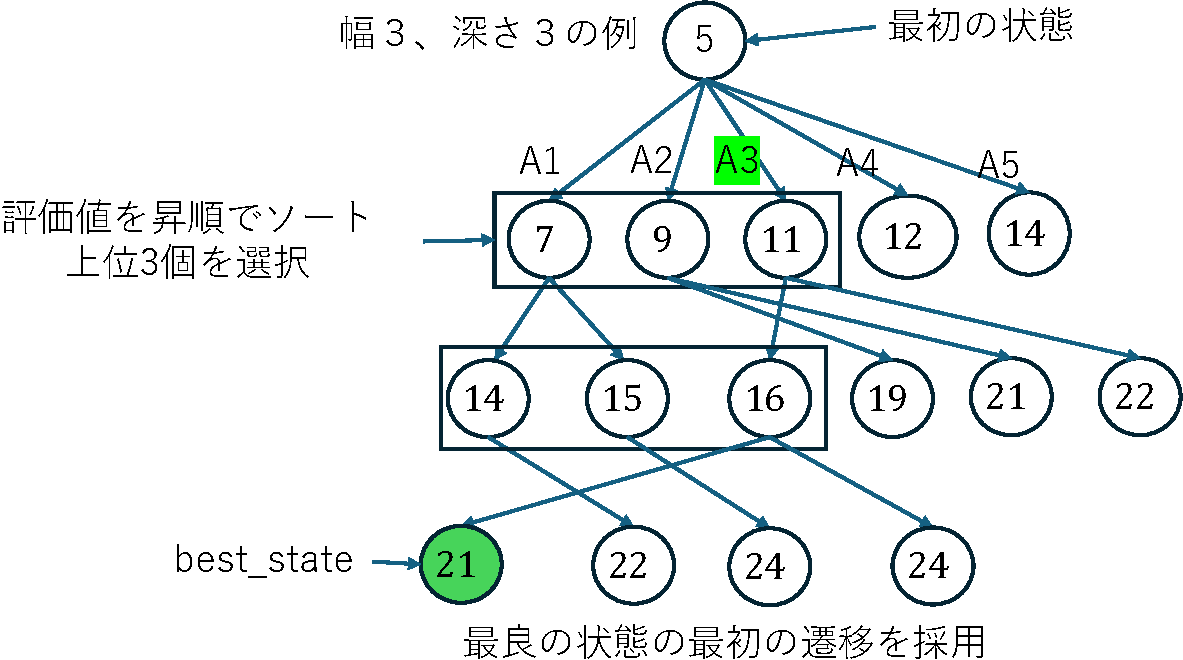
\includegraphics[width=11cm]{img/beam_search.pdf}
  \caption{深さ3,幅3の\gout{ビームサーチ}の動作例}
  \label{beam_search}
\end{figure}
図~\ref{beam_search}に深さ3,幅3の\gout{ビームサーチ}の動作例を示す.
図~\ref{beam_search}では,各ノードが状態を表している.
ノードに書かれている数字がその状態の評価値を表す.
\gout{図~\ref{beam_search}}の例では評価値が小さいものが優れた解であるとする.
初期状態からの状態の遷移をA1,A2,\dots ,A5とする.
図~\ref{beam_search}では初期状態から,5つの状態への遷移が列挙される.
探索する幅は3であるため,そのうち上位3個の状態を探索する.
上位3個の状態から\gout{遷移する状態を列挙し},再びその上位3個の状態を探索する.
この動作を繰り返し,深さ3に達したら,その時の最良の候補の最初の遷移A3を採用する.

\chapter{MCTゲートの分解手法}
本章では,既存のMCTゲートの\bout{分解手法\cite{abdessaied2016technology,baker2019decomposing,niemann2019t}}について説明する.
以降では,MCTゲートのコントロールビットの数を$c$とする.
\section{手法~1}
本節では,$c-2$個の値が不定の補助ビットを使用するMCTゲートの分解手法\cite{abdessaied2016technology}について説明する.
以降,本手法を手法~1と呼ぶ.
\bout{手法~1は,}
MCTゲートをToffoliゲートへ分解する手法\cite{barenco1995elementary}のT-depthを削減する手法である.
手法~1では,Toffoliゲートを位相のずれた$CCiZ, CCi\omega Z$ゲートに置換することで,T-depthを削減する.
\par
\mout{MCTゲートをToffoliゲートに分解した後,
これらのToffoliゲートを$CCiZ$ゲート,$CCi\omega Z$ゲートに置換する方法について説明する.
手法~1では,最初にToffolliゲートを$CCZ$ゲートとHゲートに置換する.
図~\ref{toffoli_transform}に示すように,ToffoliゲートはHゲートと$CCZ$ゲートに置換できる.
このため,図~\ref{barenco}中の,Toffoliゲートは図~\ref{toffoli_to_ccz}に示すように$CCZ$ゲートとHゲートに置換できる.}
\begin{figure}[tbp]
  \centering
  \begin{minipage}[b]{0.8\columnwidth}
    \centering
    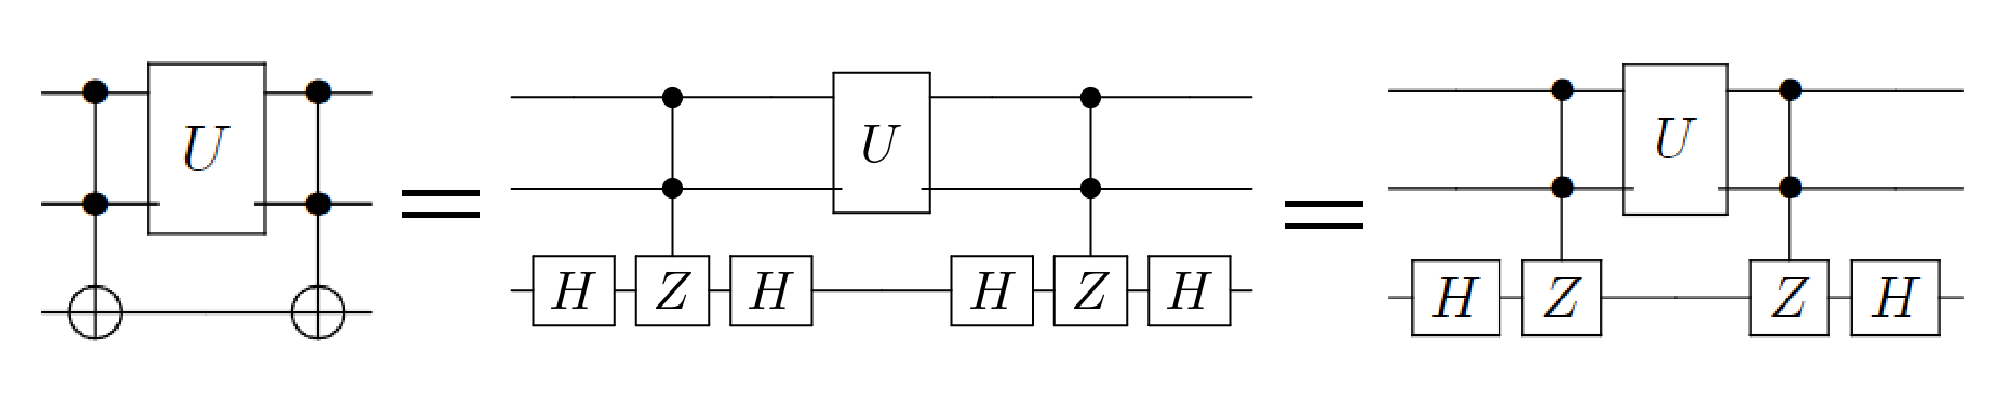
\includegraphics[width=0.9\columnwidth]{img/toffoli_transform.pdf}
    \caption{Toffoliゲートの$CCZ$ゲートへの置換}
    \label{toffoli_transform}    
  \end{minipage}
  \begin{minipage}[b]{0.4\columnwidth}
    \centering
    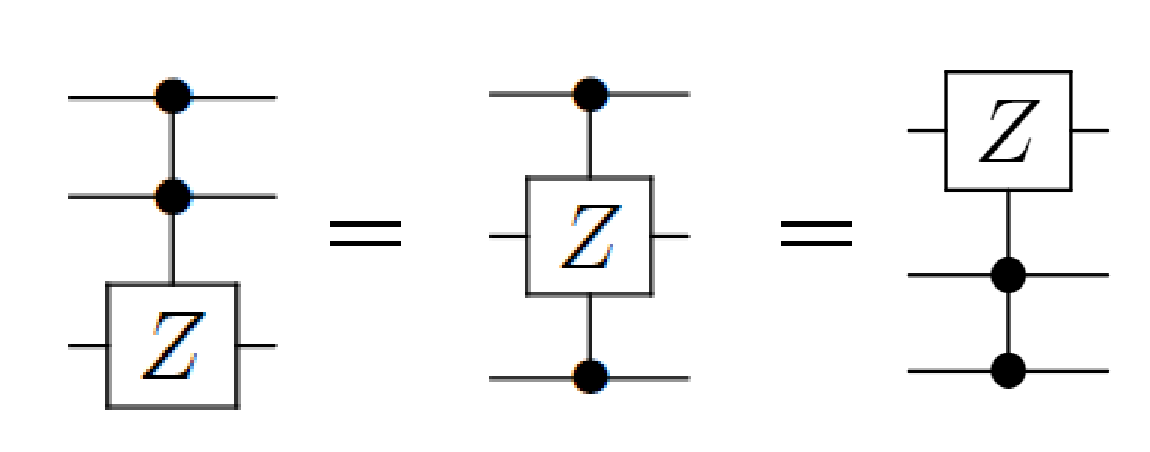
\includegraphics[width=0.9\columnwidth]{img/zgate_transform.pdf}
    \caption{$CCZ$ゲートの変形}
    \label{zgate_transform}    
  \end{minipage}
\end{figure}
\begin{figure}[tbp]
  \centering
  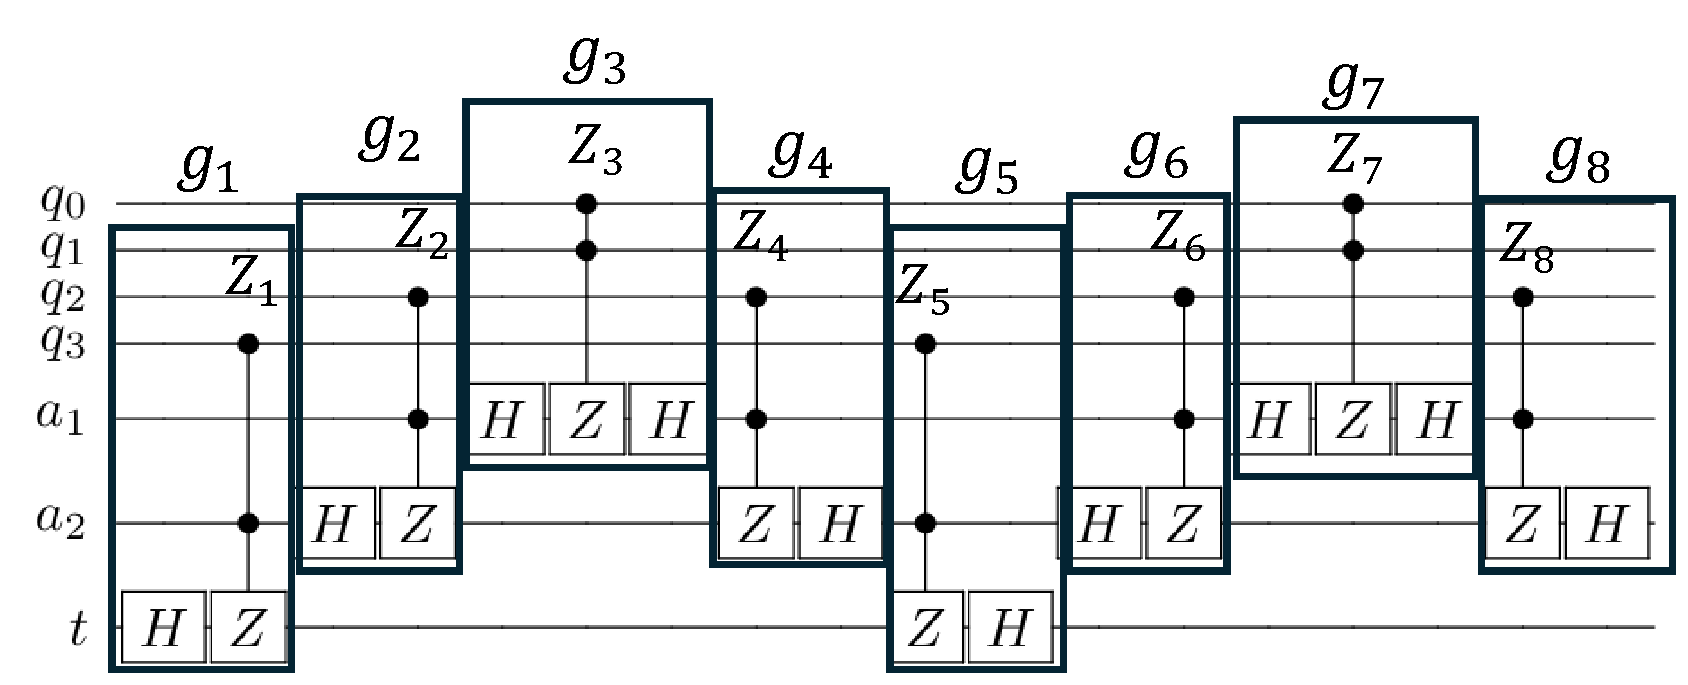
\includegraphics[width=13cm]{img/toffoli_to_ccz.pdf}
  \caption{図~\ref{barenco}のToffoliゲートを$CCZ$ゲートとHゲートに置換した例}
  \label{toffoli_to_ccz}
\end{figure} 
\par
\mout{次に,置換した$CCZ$ゲートを,$CCiZ$ゲートに置換する方法を説明する.
$CCZ$ゲートは,図~\ref{zgate_transform}に示すように,コントロールビットとターゲットビットを同一に見なすことができる.
また,図~\ref{zgate_to_iz}に示すように,$CCZ$ゲートは,
$CCiZ, CS$ゲートか,$CCiZ^{\dag}, CS^{\dag}$ゲートに置換できる.
このため,図~\ref{ccz_to_iz_cs}に示すように,図~\ref{toffoli_to_ccz}中の$CCZ$ゲートを$CCiZ, CS$ゲートと$CCiZ^{\dag}, CS^{\dag}$ゲートに置換できる.
図~\ref{ccz_to_iz_cs}では,図~\ref{toffoli_to_ccz}中の,
向かい合うゲート$\{Z_{1}. Z_{5}\}, \{Z_{2}, Z_{4}\}, \{Z_{3}, Z_{7}\},\{Z_{6}, Z_{8}\}$の組
をそれぞれ$CCiZ, CS$ゲート,$CCiZ^{\dag}, CS^{\dag}$ゲートの組に置換している.
これらの向かい合う$CCZ$ゲートを置換する際,
置換後の$CS, CS^{\dag}$ゲートの間で演算が生じない位置になるよう置換する.
例えば,$Z_{3}, Z_{7}$の組であれば,
置換後の$CS, CS^{\dag}$ゲート間で演算が生じないよう,
$CS, CS^{\dag}$ゲートのコントロールビットが$q_{0}$に,
ターゲットビットが$q_{1}$となるように置換を行う.
図~\ref{izgate_transform}のような配置の$CS,CS^{\dag}$ゲートは,互いの操作を打ち消しあうため,削除できる.
このため,図~\ref{ccz_to_iz_cs}中の,間に演算がない向かい合う$CS, CS^{\dag}$ゲート,$S_{1}, \dots, S_{8}$は削除できる.
このようにして,$CCZ$ゲートは$CCiZ$ゲートに置換できる.}
\begin{figure}[tbp]
  \centering
  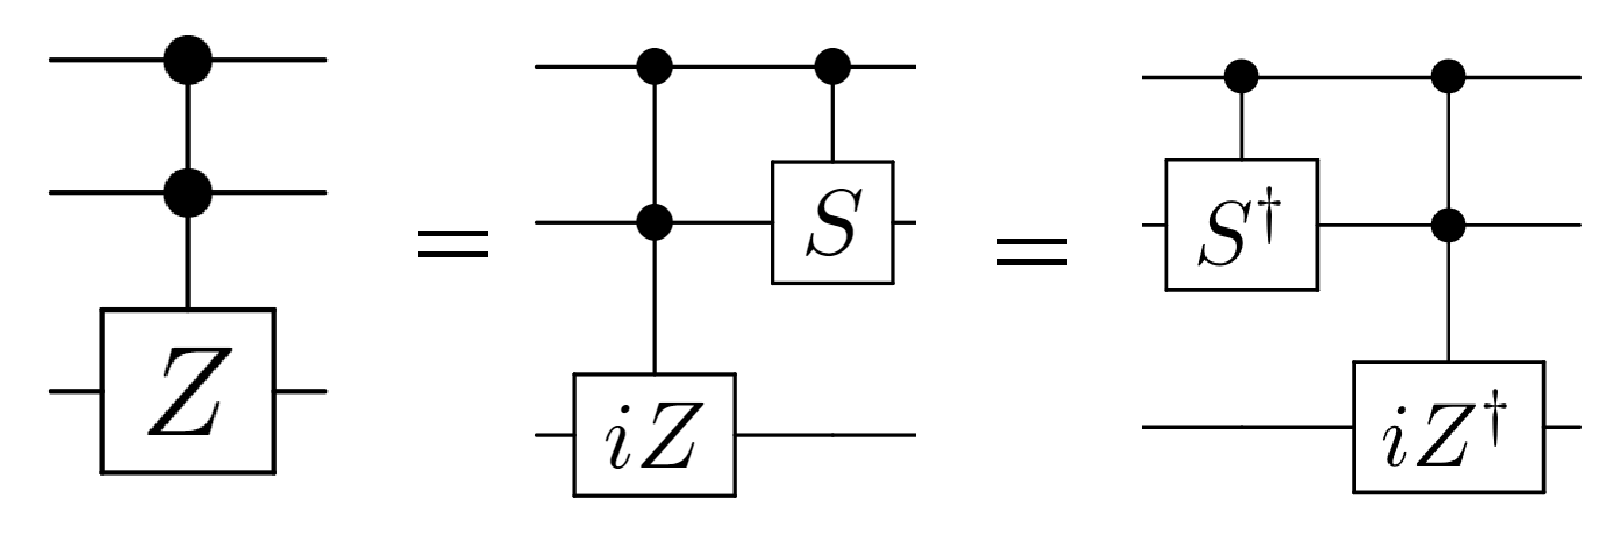
\includegraphics[width=0.5\columnwidth]{img/zgate_to_izgate.pdf}
  \caption{$CCZ$ゲートから$CCiZ, CS$ゲート,$CCiZ^{\dag}, CS^{\dag}$ゲートへの置換}
  \label{zgate_to_iz}    
\end{figure}
\begin{figure}[tbp]
    \centering
    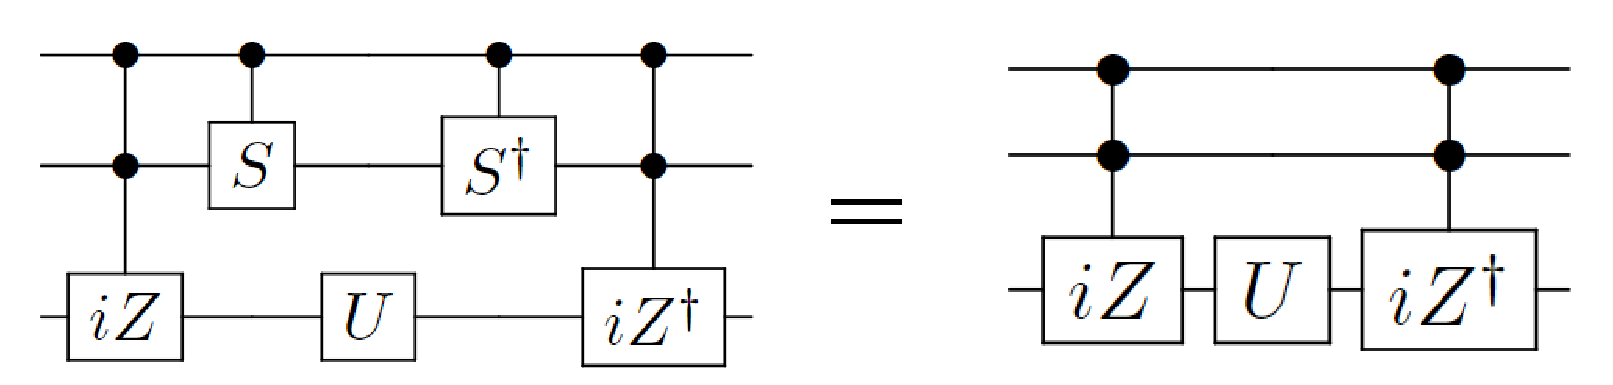
\includegraphics[width=0.5\columnwidth]{img/izgate_transformation.pdf}
    \caption{$CS, CS^{\dag}$ゲートの打ち消しあい}
    \label{izgate_transform}    
\end{figure}
\begin{figure}[tbp]
  \centering
  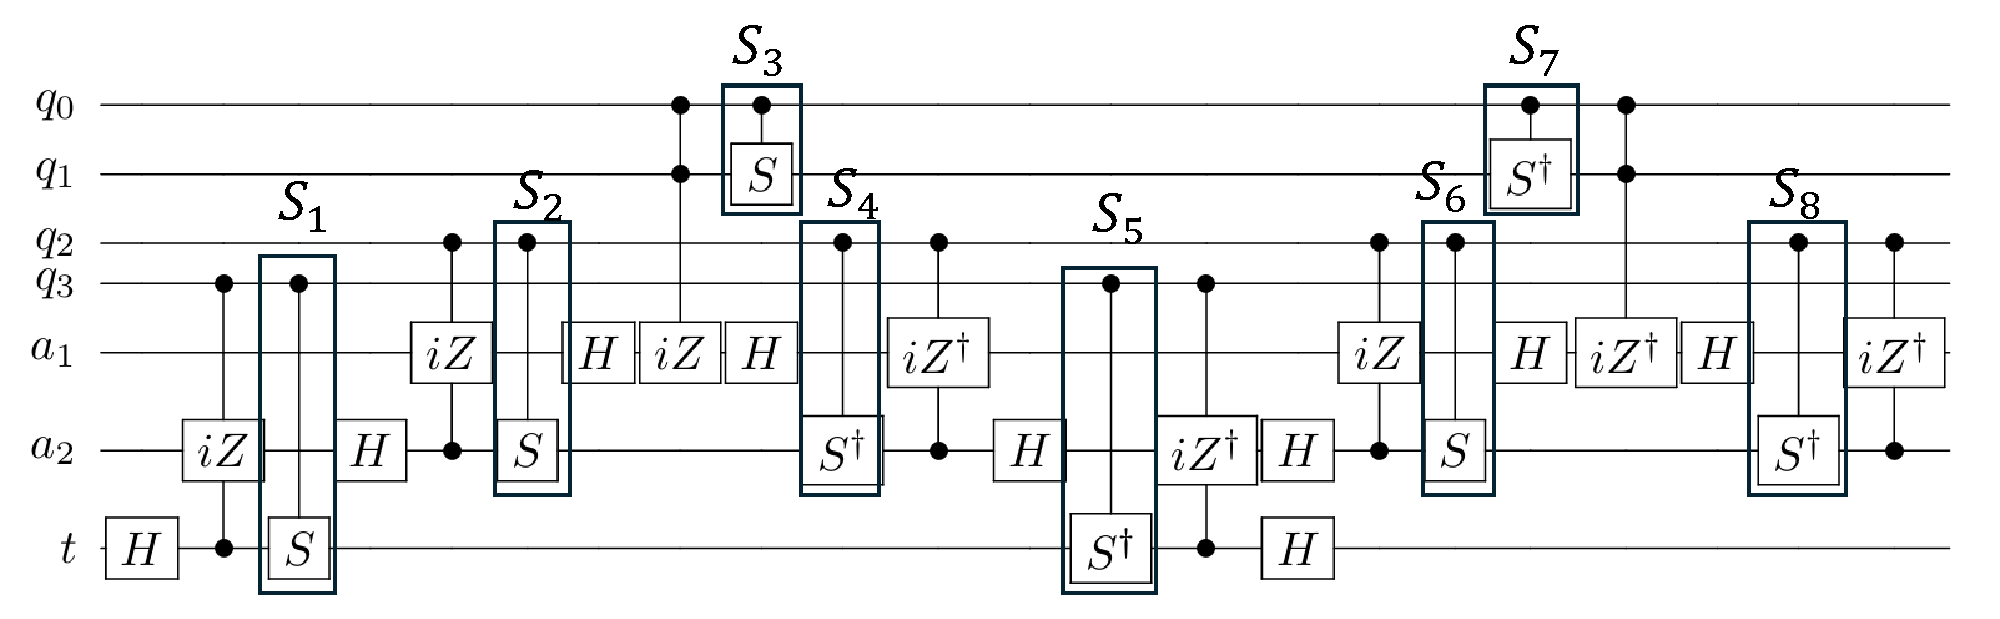
\includegraphics[width=14cm]{img/ccz_to_iz_cs.pdf}
  \caption{図~\ref{toffoli_to_ccz}の$CCZ$ゲートを$CCiZ, CS$ゲートと$CCiZ^{\dag}, CS^{\dag}$ゲートに置換した例}
  \label{ccz_to_iz_cs}
\end{figure}
\par
\mout{最後に,$CCiZ$ゲートを$CCi\omega Z$ゲートに置換する方法を説明する.
図~\ref{iz_to_iomegaz}に示すように,$CCiZ$ゲートは$CCi\omega Z$ゲートと$T^{\dag}$ゲートに置換でき,
$CCiZ^{\dag}$ゲートは$CCi\omega Z^{\dag}$ゲートと$T$ゲートに置換できる.
図~\ref{barenco_iz_to_iomegaz}に,図~\ref{ccz_to_iz_cs}の
$CCiZ, CCiZ^{\dag}$ゲートをそれぞれ,$CCi\omega Z, T^{\dag}$ゲートと$CCi\omega Z^{\dag}, T$ゲートに置換した例を示す.
図~\ref{barenco_iz_to_iomegaz}中の$T_{2}$と$T_{3}$は,それぞれの操作を打ち消しあっているため,
これらの$T, T^{\dag}$ゲートは削除できる.
図~\ref{barenco_iz_to_iomegaz}中の$T_{4}$は$T_{1}$の操作を復元する.
これらのゲートは,存在しなくても演算の結果に影響を与えることはないため,削除できる.
このように,演算に影響がない$T, T^{\dag}$ゲートを削除し,
$CCiZ$ゲートを$CCi\omega Z$ゲートに置換する.
結果として,
図~\ref{techmap}に示すように,
図~\ref{barenco}中で最も下側に位置するゲート$g_{1}, g_{5}$と,最も上側に位置するゲート$g_{3}, g_{7}$は$CCiZ, CCiZ^{\dag}$ゲートに置換できる.
また,図~\ref{barenco}中のゲート$g_{2}, g_{4}$と$g_{6}, g_{8}$は,それぞれ$CCi\omega Z, CCi\omega Z^{\dag}$ゲートに置換できる.}
\begin{figure}[tbp]
  \centering
  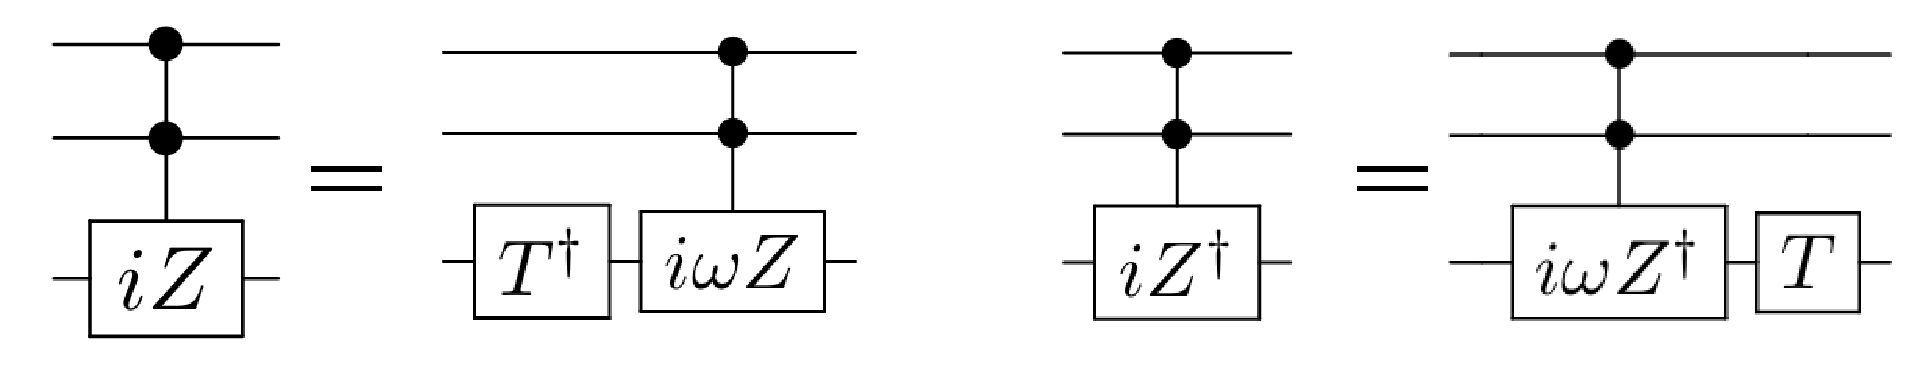
\includegraphics[width=11cm]{img/iz_to_iomegaz.pdf}
  \caption{\bout{$CCiZ$ゲートの$CCi\omega Z, T^{\dag}$ゲートへの置換と,$CCiZ^{\dag}$ゲートの$CCi\omega Z^{\dag}, T$ゲートへの置換}}
  \label{iz_to_iomegaz}
\end{figure}
\begin{figure}[tbp]
  \centering
  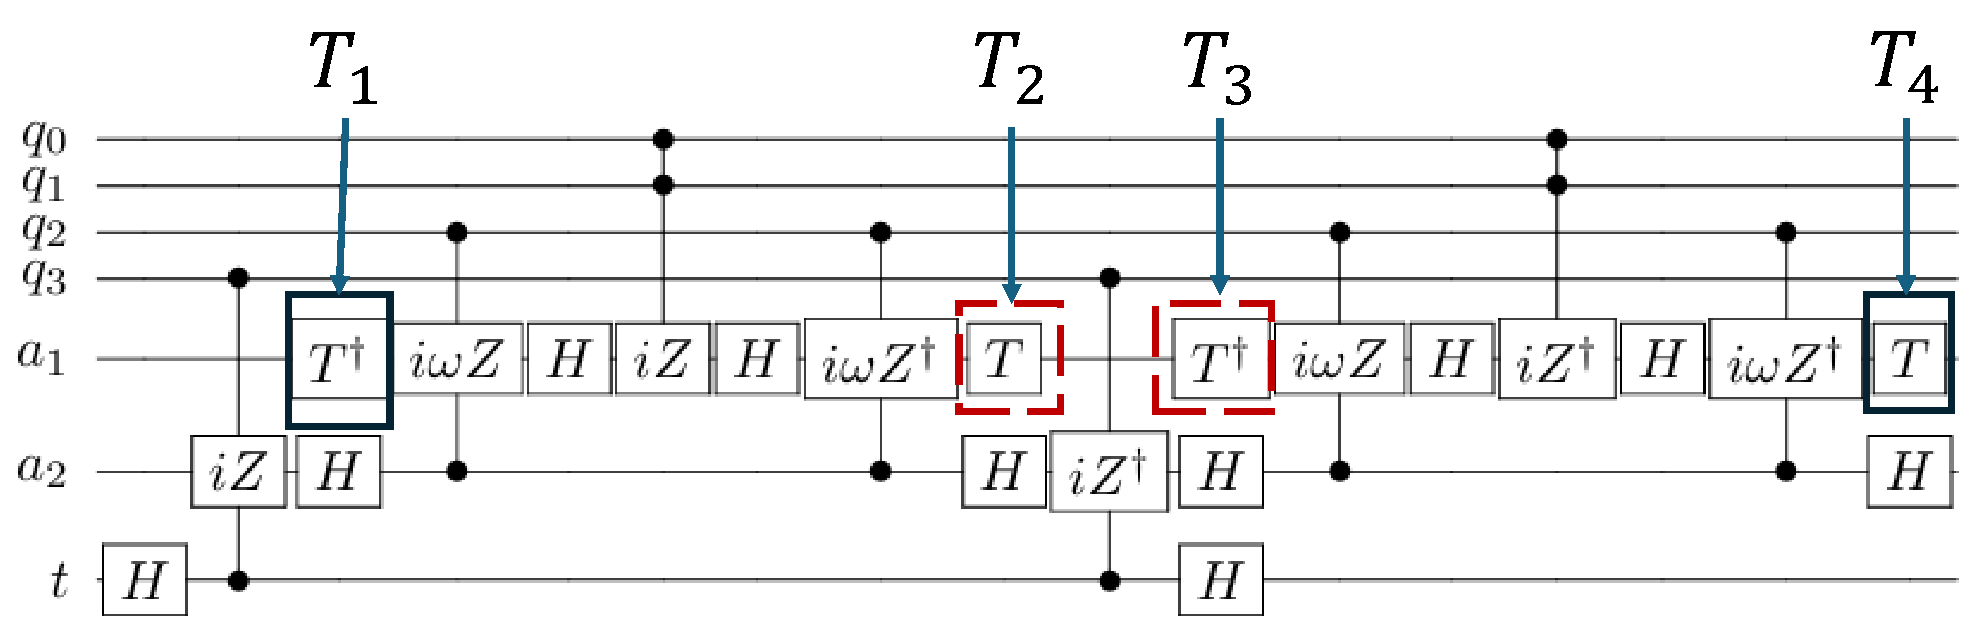
\includegraphics[width=14cm]{img/barenco_iz_to_iomegaz.pdf}
  \caption{図~\ref{ccz_to_iz_cs}の$CCiZ, CCiZ^{\dag}$ゲートをそれぞれ,$CCi\omega Z, T^{\dag}$ゲートと$CCi\omega Z^{\dag}, T$ゲートに置換した例}
  \label{barenco_iz_to_iomegaz}
\end{figure}
\begin{figure}[tbp]
  \centering
  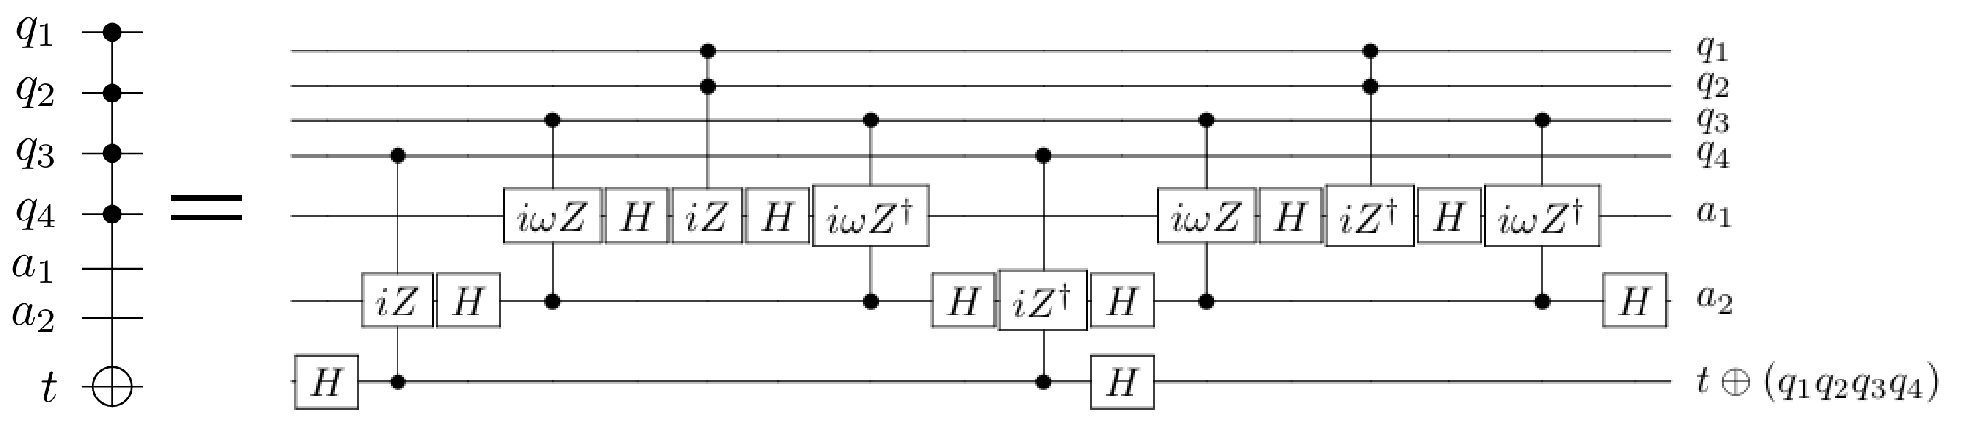
\includegraphics[width=0.9\columnwidth]{img/techmap.pdf}
  \caption{$c=4$のMCTゲートへの手法~1の適用例}
  \label{techmap}
\end{figure}
\par
手法~1は,MCTゲートを$c-2$個の補助ビットを用いて,
% 分解の説明をする普通に全部説明したほうが楽かも
4個の$CCiZ$ゲートと,$4(c-3)$個の$CCi\omega Z$ゲートに分解する.
$CCiZ$ゲートと,$CCi\omega Z$ゲートのClifford+Tへの分解をそれぞれ図~\ref{cciz},図~\ref{cciomegaz}に示す.
$CCiZ$ゲートのT-depthは2,$CCi\omega Z$ゲートのT-depthは1である.
そのため,手法~1で分解したMCTゲートの最大のT-depthは,$4(c-1)$である.
\begin{figure}[tbp]
  \centering
  \begin{minipage}[b]{0.49\columnwidth}
    \centering
    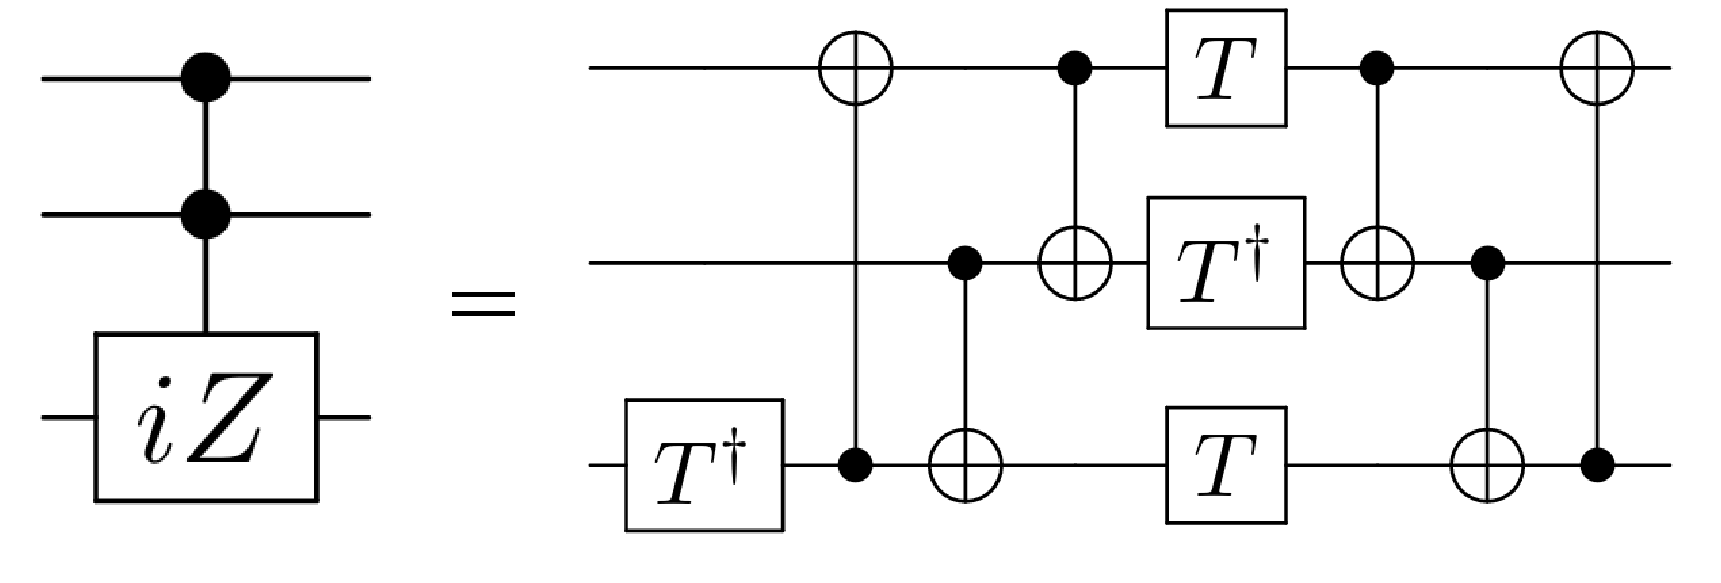
\includegraphics[width=0.9\columnwidth]{img/cciz.pdf}
    \caption{$CCiZ$ゲートのClifford+Tへの分解}
    \label{cciz}    
  \end{minipage}
  \begin{minipage}[b]{0.49\columnwidth}
    \centering
    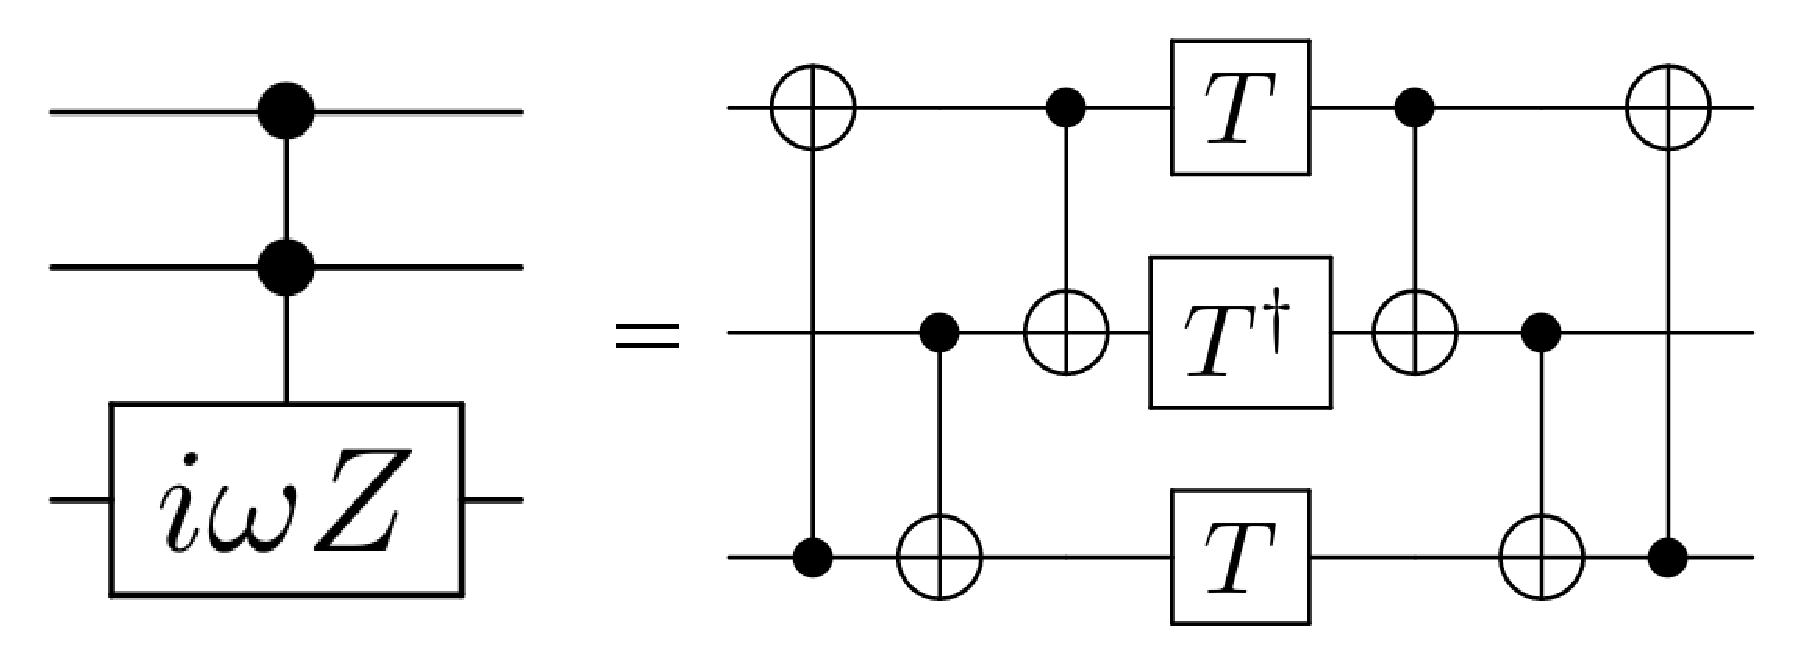
\includegraphics[width=0.9\columnwidth]{img/cciomegaz.pdf}
    \caption{$CCi\omega Z$ゲートのClifford+Tへの分解}
    \label{cciomegaz}    
  \end{minipage}
\end{figure}
\section{手法~2}
本節では,1個の値が不定の補助ビットを使用する分解手法\cite{abdessaied2016technology}について説明する.
以降,本手法を手法~2と呼ぶ.
\par
値が不定の補助ビットが\bout{$c-2$個未満のとき},MCTゲートを手法~1で分解することができない.
%コントロールビットを二つに分解することを説明する.
\bout{そこで,$c$個のコントロールビットを2つのビットの集合に分割する.
このとき,2つのビットの集合の要素数の差が1個以内となるよう分割する.}
そして,図~\ref{mimap}に示すように,
分割したビットの集合をコントロールビットに持つ4つのMCTゲート
$g_{1}, g_{2}, g_{3}, g_{4}$と4つの$C\omega S$ゲートにMCTゲートを一度分解する.
\begin{figure}[tbp]
  \centering
  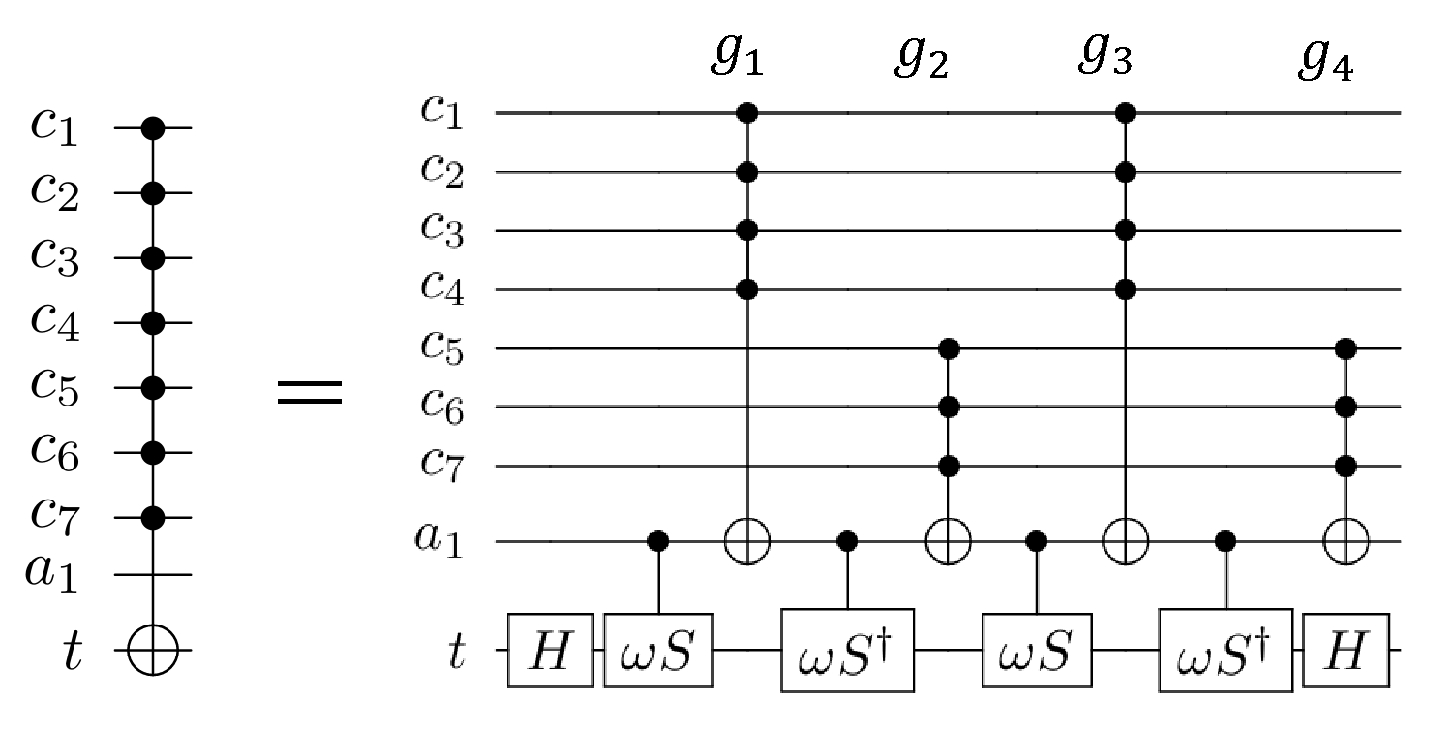
\includegraphics[width=11cm]{img/mimapping.pdf}
  \caption{$c=7$のMCTゲートへの手法~2の適用例}
  \label{mimap}
\end{figure}
ここで,$g_{3}$は$g_{1}$の,$g_{4}$は$g_{2}$の複製である.
\begin{figure}[tbp]
  \centering
  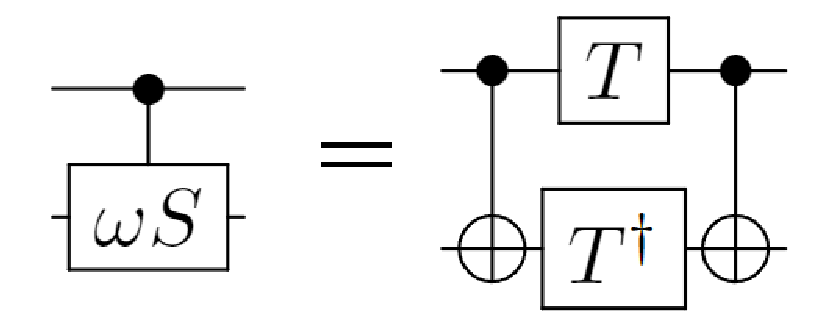
\includegraphics[width=5cm]{img/comegas.pdf}
  \caption{$C\omega S$ゲートのClifford+Tへの分解}
  \label{comegas}
\end{figure}
図~\ref{comegas}に示すように,
$C\omega S$ゲートは,補助ビットを用いずに,直接Clifford+Tへ分解できるゲートである.
手法~2では,
この分解した4つのMCTゲートに対し,手法~1を適用することで,MCTゲートをClifford+Tへ分解することができる.
\par
手法~2では,図~\ref{mimap}の$g_{3}$を$g_{1}$の分解に対し,$g_{4}$を$g_{2}$の分解に対し,
同じ補助ビットを使い,逆変換のゲートに置換したうえで,逆順に分解することで,T-depthを削減する.
\mout{
図~\ref{mimap_g2_g4}に
図~\ref{mimap}中の$g_{2}$を分解し,
$g_{4}$を$g_{2}$の分解に対し,逆変換のゲートに置換し,逆順に分解した例を示す.
図~\ref{mimap_g2_g4}の$G_{2}, G_{4}$は,$g_{2}, g_{4}$の分解を表す.
$G_{4}$は$G_{2}$を構成するゲートを逆変換のゲートに置換し,逆順にしたものである.}
\begin{figure}[tbp]
  \centering
  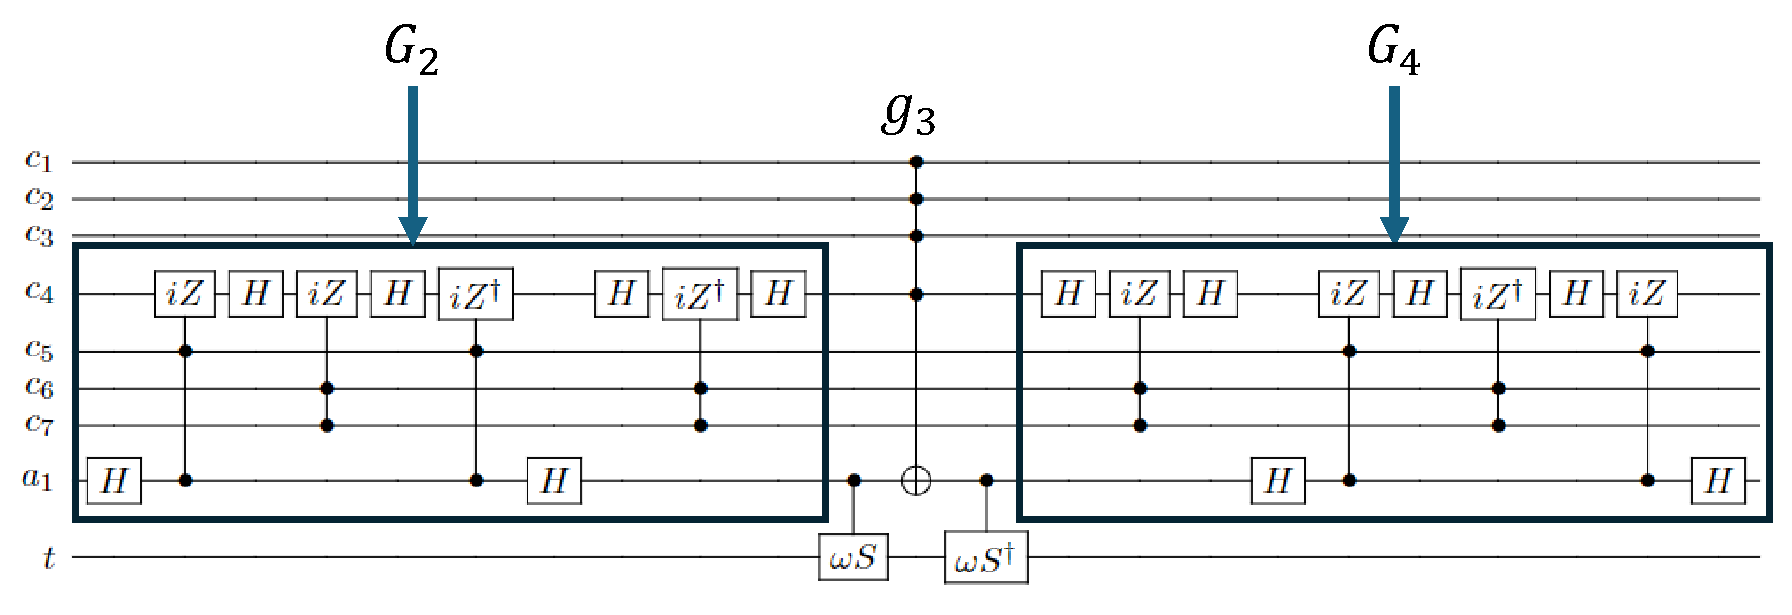
\includegraphics[width=15cm]{img/mimap_g2_g4.pdf}
  \caption{\mout{図~\ref{mimap}の$g_{2}$を分解し,$g_{4}$を$g_{2}$の分解に対し逆変換のゲートに置換し,逆順に分解した例}}
  \label{mimap_g2_g4}
\end{figure}
図~\ref{iz_to_iomegaz}に示すように,
\bout{$CCiZゲート$と$CCiZ^{\dag}$ゲートはそれぞれ,
$CCi\omega Z, T^{\dag}$ゲートと$CCi\omega Z^{\dag}, T$ゲートに置換できる.}
図~\ref{mimap_g2_g4}の\bout{$CCiZゲート$と$CCiZ^{\dag}$ゲートをそれぞれ,
$CCi\omega Z, T^{\dag}$と$CCi\omega Z^{\dag}, T$ゲートに}
置換した例を図~\ref{mimap_g2_g4_trans}に示す.
\mout{
図~\ref{mimap_g2_g4_trans}の$T$ゲート$T_{4}$は,
$T^{\dag}$ゲート$T_{1}$の操作を復元する.
これらのゲートは,存在しなくても演算の結果に影響を与えることはないため,削除できる.
同様に図~\ref{mimap_g2_g4_trans}の$T_{2}, T_{3}$についても削除できる}.
\par
このようにして,$g_{1}, g_{3}$の組と$g_{2}, g_{4}$の組を分解することで,
合計8つの$CCiZ, CCiZ^{\dag}$ゲートを$CCi\omega Z, CCi\omega Z^{\dag}$ゲートへ置換でき,\mout{置換を行う前からT-depthを8削減できる.
コントロールビットの差を一つ許容して均等に分割するため,
置換を行う前の4つのMCTゲートを手法1で分解した合計のT-depthは,
$2 \cdot  4(\lfloor \frac{c}{2}  \rfloor -1) +2\cdot 4(\lceil \frac{c}{2} \rceil -1)=8(c-1)$となる.
また,4つの$C\omega S$ゲートを使用しているため,これらのゲートの合計のT-depthは$4$である.}
このため,手法~2を用いてコントロールビット数が$c$個のMCTゲートを
分解したときの最大のT-depthは$8(c-1)-8+4=8c-20$となる.
\begin{figure}[tbp]
  \centering
  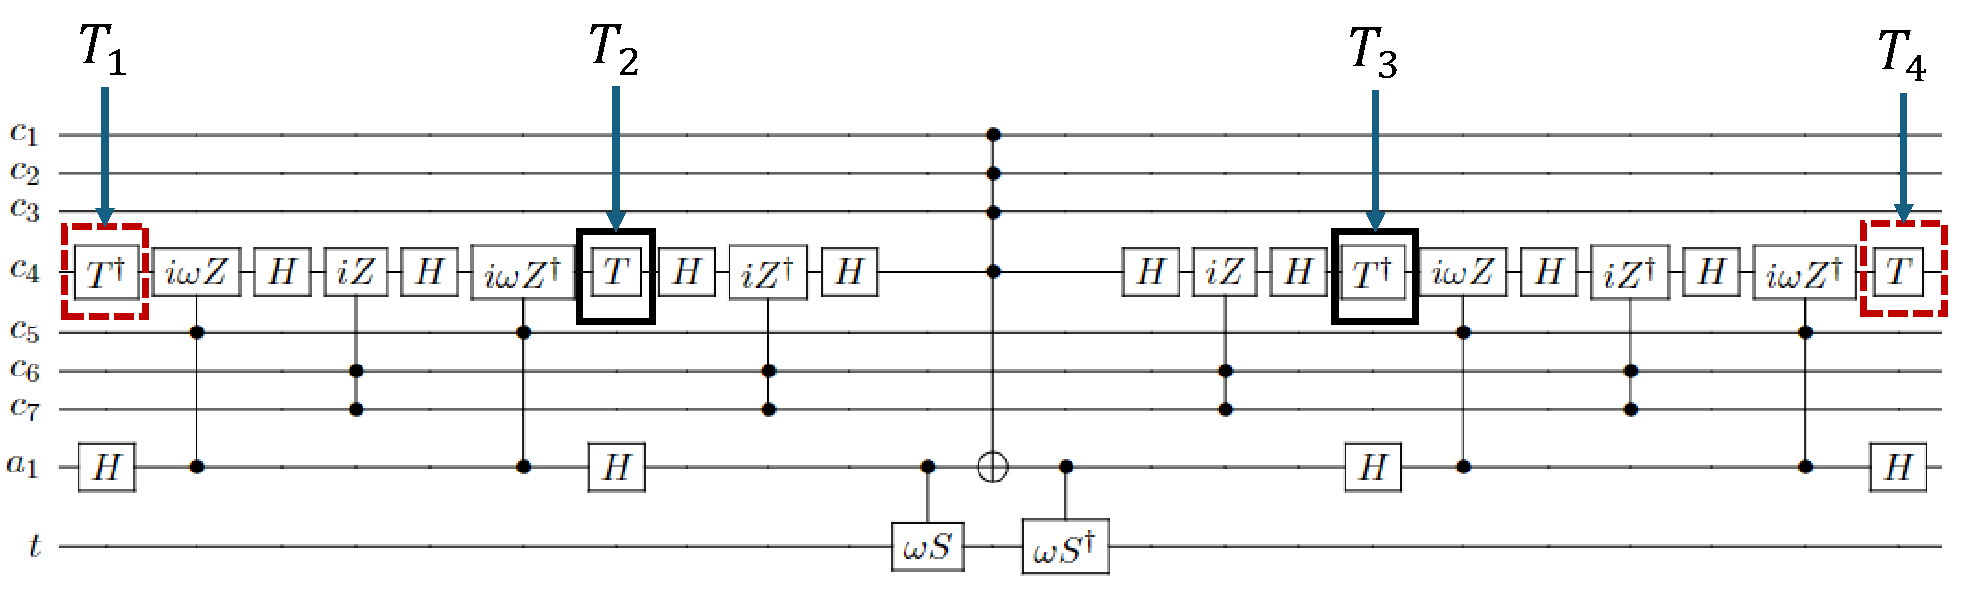
\includegraphics[width=18cm]{img/mimap_g2_g4_transform.pdf}
  \caption{図~\ref{mimap_g2_g4}の\bout{$CCiZ, CCiZ^{\dag}$ゲートをそれぞれ,$CCi\omega Z, T^{\dag}$ゲートと$CCi\omega Z^{\dag}, T$ゲートへ置換した例}}
  \label{mimap_g2_g4_trans}
\end{figure}
\section{手法~3}
本節では,2から$c-3$個の値が不定の補助ビットを使用し,MCTゲートを分解する手法\cite{baker2019decomposing}について説明する.
以降,本手法を手法~3と呼ぶ.
図~\ref{baker}に示すように,
\mout{\rout{必要な複製の数}が少ないMCTゲート$g_{1}$または$g_{4}$に,
多くのコントロールビットを使用し,分解することで,T-depthを削減する手法が手法~3である.
図~\ref{baker}の$g_{1}$の複製は$g_{7}$のみであるが,
$g_{2}$の複製は,$g_{6}, g_{8}, g_{13}$であるため,
$g_{1}$はその複製の数が少ないゲートといえる.
$g_{4}$についても,複製は$g_{10}$のみである.}
\par
手法~3の分解方法について説明する.
分解するMCTゲートの$c$個のコントロールビットの集合を$C$とする.
分解するMCTゲートのターゲットビットを$t$とする.
\mout{MCTゲートの分解に使用できる,$m$個の値が不定の補助ビットを$a_{1}, a_{2}, \dots, a_{m}$とする.}
図~\ref{baker}のように,$g_{1}, g_{2}, g_{3}, g_{4}$の配置が決定すれば,
$g_{4}$より右側にあるゲートは,$g_{1}, g_{2}, g_{3}, g_{4}$の複製であるため手法~3の分解は\rout{決定}できる.
すなわち,左側から$m+1$個分のゲートを構成するビットの配置が決定すれば,手法~3の分解を\rout{決定}できる.
この左側から$m+1$個のMCTゲートをそれぞれ$g_{1},\dots,g_{m+1}$とする.
$g_{1},\dots ,g_{m+1}$の持つ,コントロールビットの集合をそれぞれ$C_{1}, C_{2}, \dots ,C_{m+1}$で表す.
また,集合の要素数は,$|C_{i}|$で表す.
ここで,次の手順に則り,コントロールビットの集合$C_{1},\dots ,C_{m+1}$を構成するビットを決定する.
\begin{enumerate}[手順1]
  \item $C_{1}, \dots ,C_{m}$に$a_{1},\dots,a_{m}$を一つずつ移動する.
  \item $C_{1},\dots, C_{m+1}$の要素数が全て2になるように,\mout{$C$から$C_{i}$に要素を移動する.}
  \item $C_{1}$が$|C_{1}|-2 \leq c+m-|C_{1}|$である限り,\mout{$C$から$C_{1}$に要素を移動する.}
  \item $|C|=0$でなければ,\mout{$C_{m+1}$に,$C$の残りの要素を移動する.}
\end{enumerate}
\par
次に,$g_{1},\dots ,g_{m+1}$のターゲットビットの決定方法について説明する.
$g_{1}$のターゲットビットは,分解前のMCTゲートのターゲットビット$t$である.
$g_{i\geq 2}$のターゲットビットは,手順1で分配した$C_{i-1}$\mout{に含まれるビットである.}
このようにして,$g_{1},\dots, g_{m+1}$のビットの配置を決定する.
\par
$g_{1},\dots ,g_{m+1}$の構成するビットが決定すれば,
回路の左側から式~\ref{eq:bakerhaiti}の順でゲートを配置する.
\begin{equation}\label{eq:bakerhaiti}
  \{g_{1}, g_{2}, \dots, g_{m+1}\},\{g_{m},g_{m-1}, \dots, g_{1}\}, \{g_{2}, g_{3} \dots, g_{m+1}\}, \{g_{m}, g_{m-1}, \dots, g_{2}\}
\end{equation}
配置したゲートのうちコントロールビットが3個以上のゲートに関しては,手法~1により分解する.
\begin{figure}[tbp]
  \centering
  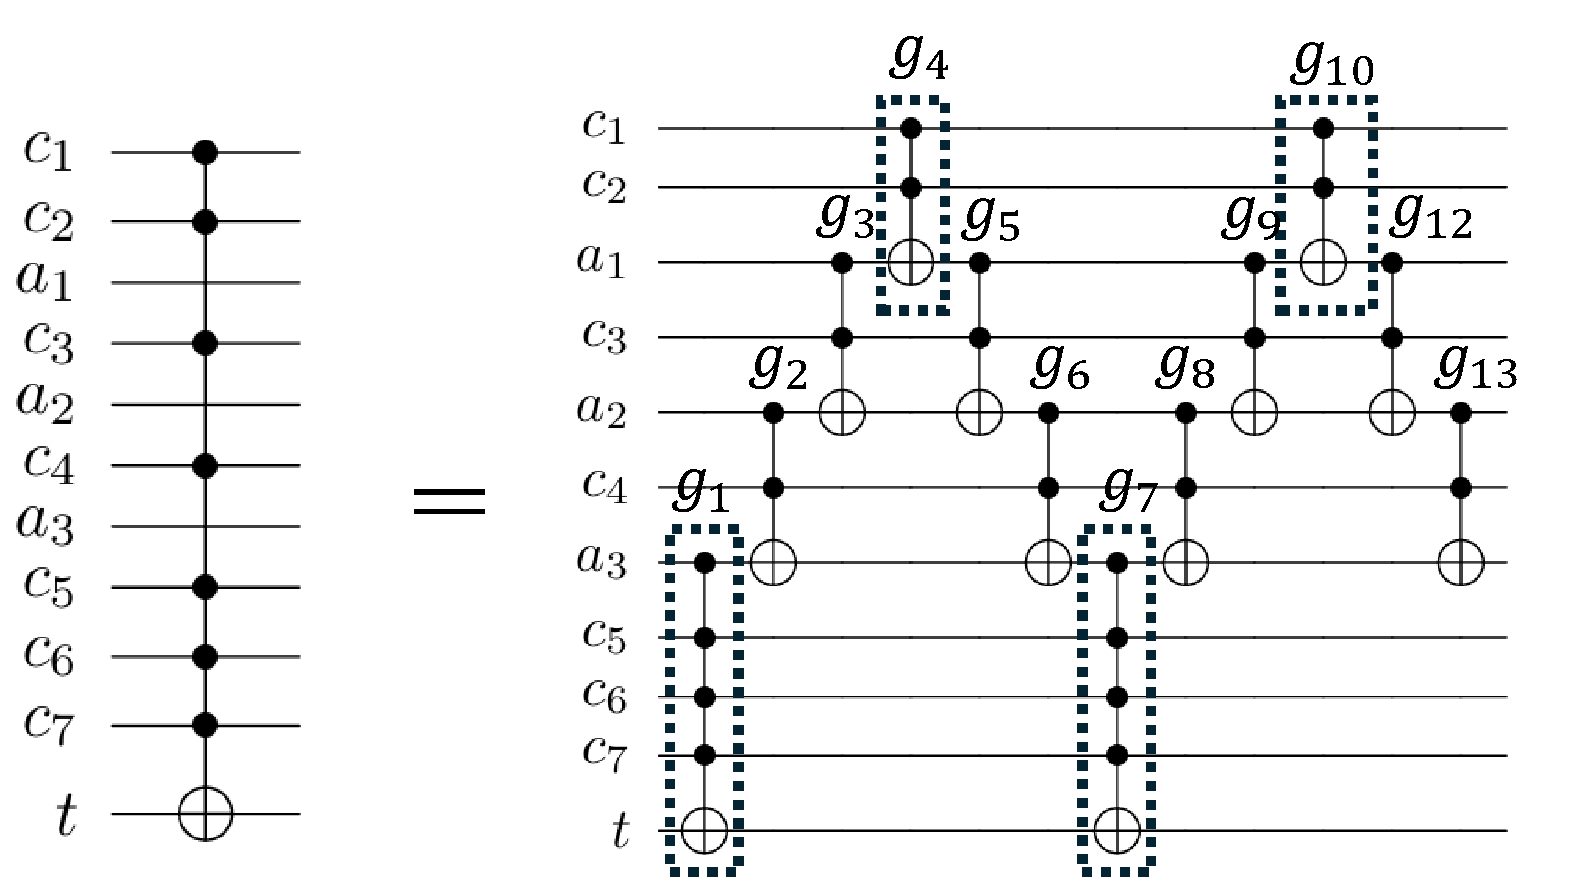
\includegraphics[width=10cm]{img/baker.pdf}
  \caption{値が不定の補助ビットが3個の時の$c=7$のMCTゲートへの手法~3の適用例}
  \label{baker}
\end{figure}
\par
MCTゲートに手法~3の分解を適用した際に現れるToffoliゲートは,$CCiZ, CCi\omega Z$ゲートに置換できる.
この方法について説明する.
まず,図~\ref{baker}上のToffoliゲートは,$CCiZ, CCiZ^{\dag}$ゲートに置換することができる.
図~\ref{baker_cciz}にその例を示す.
\begin{figure}[tbp]
  \centering
  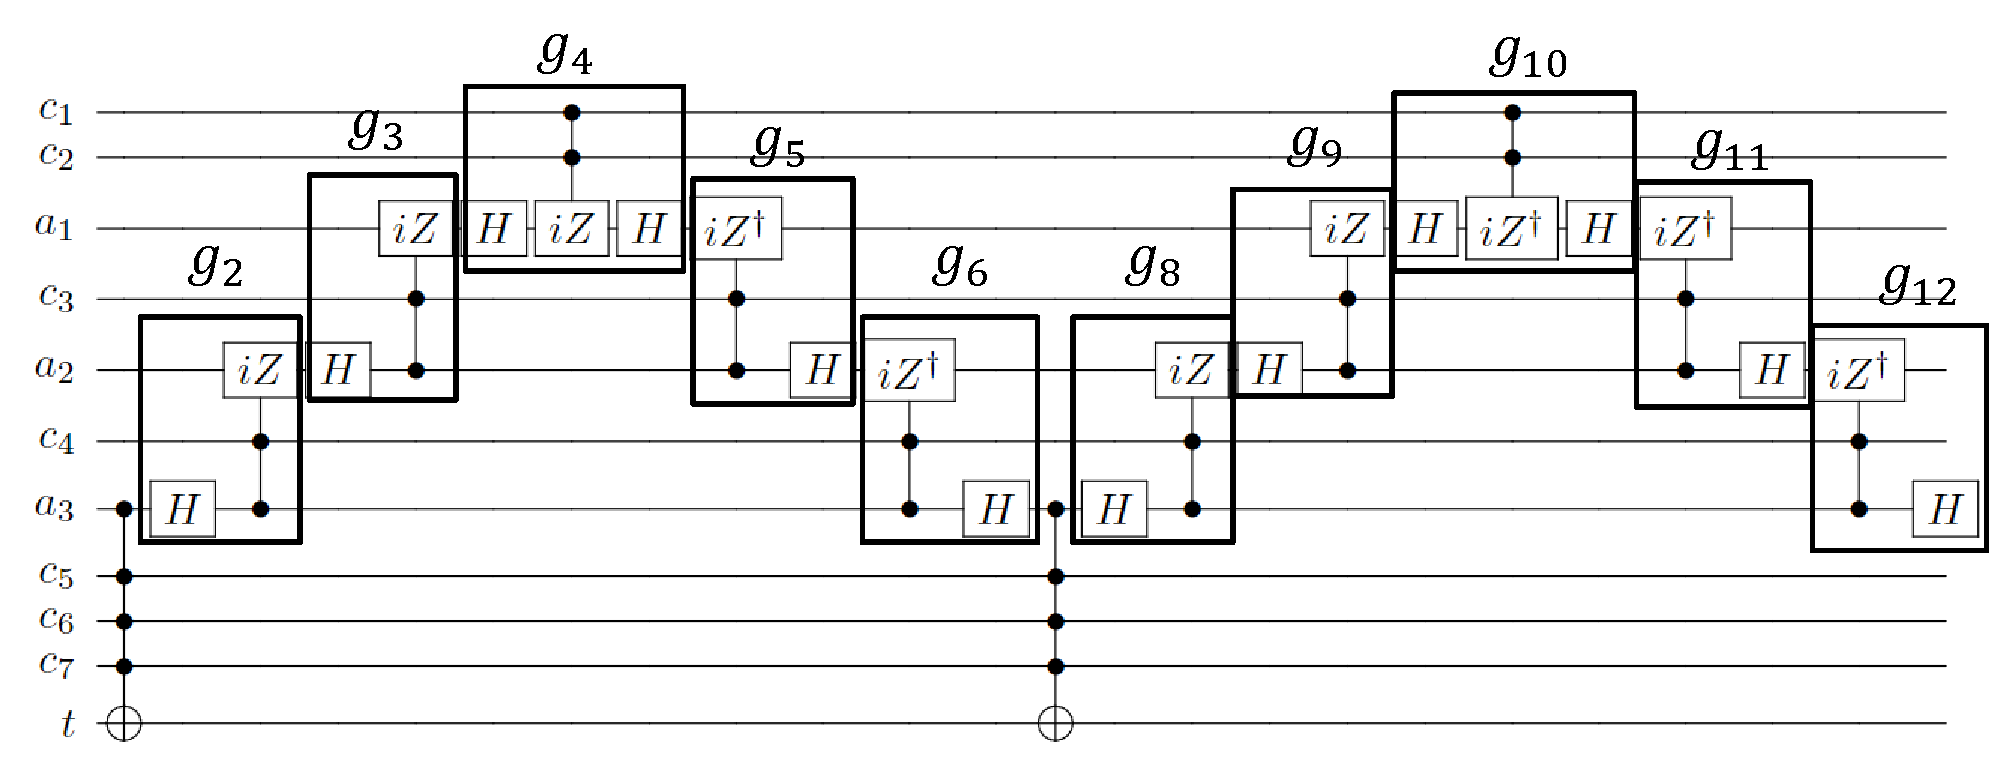
\includegraphics[width=15cm]{img/baker_izgate_transform.pdf}
  \caption{図~\ref{baker}のToffoliゲートの$CCiZ$ゲートへの置換}
  \label{baker_cciz}
\end{figure}
同じビットを入力と出力に持つToffoliゲートの組は,
図~\ref{toffoli_transform}のように$CCZ$ゲートに置換できる.
図~\ref{zgate_transform}に示すように,
$CCZ$ゲートは,ターゲットビットとコントロールビットを同一に見なすことができる.
図~\ref{zgate_to_iz}に示すように,$CCZ$ゲートは,$CCiZ$ゲートと$CS$ゲートか,$CCiZ^{\dag}$ゲートと$CS^{\dag}$ゲートに置換できる.
図~\ref{izgate_transform}に示すような配置の,$CS$ゲートと,$CS^{\dag}$ゲートは,互いの操作を打ち消しあう.
そのため,$CS$ゲートと,$CS^{\dag}$ゲートを消去しても同じ演算を表現できる.
このように,同じ入力と出力を持つToffoliゲートの組を,$CCiZ, CCiZ^{\dag}$ゲートの組に置換することができる.
そのため,図~\ref{baker}のToffoliゲートを図~\ref{baker_cciz}のように$CCiZ, CCiZ^{\dag}$ゲートに置換できる.
\par
図~\ref{baker_cciomegaz}に示すように,
図~\ref{baker_cciz}の
\bout{$CCiZ, CCiZ^{\dag}$ゲートはそれぞれ,$CCi\omega Z$ゲートと$T^{\dag}$ゲート, 
$CCi\omega Z^{\dag}$ゲートと$T$ゲートに置換できる.}
図~\ref{baker_cciomegaz}の
\mout{
$T, T^{\dag}$ゲート$T_{3}, T_{6}$と$T_{4}, T_{5}$は,互いの演算を打ち消し合うため,削除できる.
また,図~\ref{baker_cciomegaz}中の
$T^{\dag}, T$ゲート$T_{1}, T_{8}$と,$T_{2}, T_{7}$についても,
左側の$T_{1}, T_{2}$の\bout{$T^{\dag}$}ゲートの演算を右側の$T_{7}, T_{8}$の\bout{$T$ゲート}が復元している.}
これらのゲートが存在しなくても演算の結果に影響を与えることがないため,これらのゲートについても削除できる.
このようにして,手法~3の分解で現れるToffoliゲートは,$CCiZ, CCi\omega Z$ゲートに置換することができる.
\begin{figure}[tbp]
  \centering
  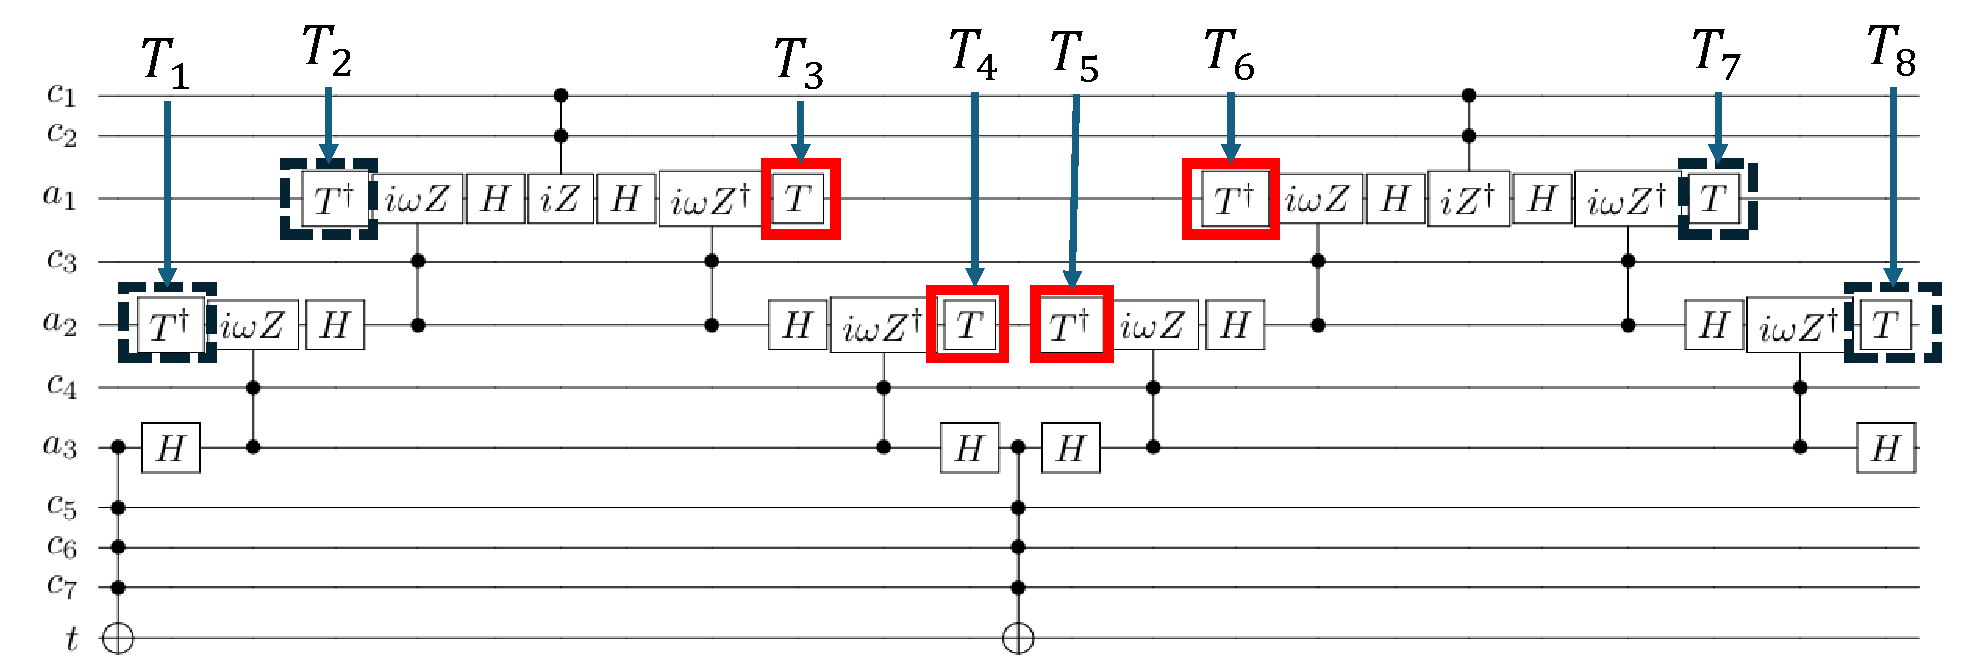
\includegraphics[width=15cm]{img/baker_iomegaz.pdf}
  \caption{図~\ref{baker_cciz}の\bout{$CCiZ, CCiZ^{\dag}$ゲートをそれぞれ,$CCi\omega Z, T^{\dag}$ゲートと$CCi\omega Z^{\dag}, T$ゲートに置換した例}}
  \label{baker_cciomegaz}
\end{figure}
\section{手法~4}
本節では,
値が0の補助ビットを用いたMCTゲートの分解手法\cite{niemann2019t}について説明する.
以降,本手法を手法~4と呼ぶ.
手法~4は,分解に使用する値が0の補助ビットの数$k$に\mout{よって場合分けして,}MCTゲートの分解を行う.
また,分解に使用する値が不定の補助ビット数を$d$とする.
$k$個の値が0の補助ビットを$a_{1},\dots, a_{k}$とする.分解を行うMCTゲートのコントロールビット数を$c$とする.
\subsection*{$1\leq k \leq \frac{c}{2}$の場合}
$1\leq k \leq \frac{c}{2}$の場合,
図~\ref{niemann}に示すように,分解するMCTゲートを3段のMCTゲートに分解する.
分解したMCTゲートそれぞれに,手法~1を適用し分解を行う.
手法~4では,図~\ref{niemann}のように,
$k$の数だけ1,3段目にMCTゲートを並列に配置することで,T-depthを削減する.
\par
MCTゲートを3段に分解する方法について説明する.
まず,分解するMCTゲートの$c$個のコントロールビットを
$k+1$個のコントロールビットの集合$C_{1},\dots,C_{k+1}$に分割する.
この分割したコントロールビットの集合の要素数は$|C_{i}|$と表す.
3段のMCTゲートの配置は次の通りである.
\begin{enumerate}[1段目]
  \item $C_{1},\dots, C_{k}$をそれぞれのコントロールビットとし,$a_{1},\dots,a_{k}$を
  それぞれのターゲットビットとする$k$個のMCTゲートを配置.
  \item $C_{k+1}$と$k$個の補助ビット$a_{1},\dots,a_{k}$をコントロールビットとし,
  ターゲットビットを元のMCTゲートのターゲットビット$t$とするMCTゲートを2段目に配置する.
  \item 3段目には1段目と同じ$k$個のMCTゲートを配置する.
  3段目のMCTゲートにより値が0の補助ビットの値を0に復元する.
\end{enumerate}
\begin{figure}[tbp]
  \centering
  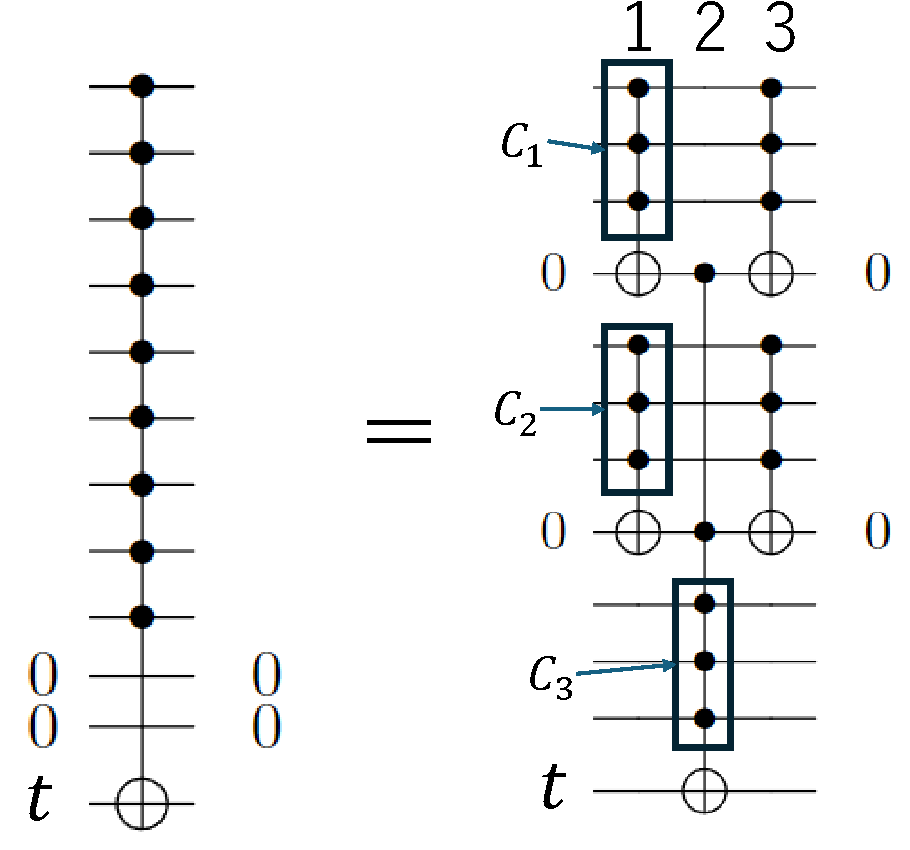
\includegraphics[width=6cm]{img/niemann.pdf}
  \caption{2つの値が0の補助ビットを用いた$c=9$のMCTゲートの分解例}
  \label{niemann}
\end{figure}
\par
3段に配置したMCTゲートの分解には,手法~1を用いる.
従って,これらのMCTゲートを分解するには,
それぞれのコントロールビットの数に応じた,値が不定の補助ビットが必要である.
各段に必要な値が不定の補助ビットの数を考慮して,
$C_{1},\dots,C_{k+1}$を決定する必要がある.
\par
2段目のMCTゲートは$k+|C_{k+1}|$個のコントロールビットを持つ.
そのため,2段目のMCTゲートに手法~1を適用するには,
$k+|C_{k+1}-2|$個の値が不定の補助ビットが必要である.
2段目のMCTゲートで使用されていないビットは,値が不定の補助ビットとして使用できる.
そのため,1段目でコントロールビットとして使用されている,
$|C_{1}|+,\dots, +|C_{k}|$個のビットは,
2段目のMCTゲートで値が不定の補助ビットとして使用できる.
2段目のMCTゲートに手法~1の分解を適用するには,
式~\ref{eq:2danme}を満たす必要がある.
\begin{equation}\label{eq:2danme}
  d+|C_{1}|+\dots +|C_{k}|\geq (k+|C_{k+1}|)-2
\end{equation}
\par
1,3段目のMCTゲートに手法~1を適用するには,
$(|C_{1}|-2)+\dots+(|C_{k}|-2)$個の値が不定の補助ビットが必要である.
1,3段目で用いられていないビットは値が不定の補助ビットとして利用できる.
そのため,
2段目でコントロールビットとして用いられる$|C_{k+1}|$個のビットと
2段目のターゲットビット$t$が値が不定の補助ビットとして利用できる.
加えて,分解に使用する値が不定の補助ビットの数$d$を考慮すると,1,3段目のMCTゲートに対して手法~1を適用するには,
式\ref{eq:13danme}を満たさなければならない.
\begin{eqnarray}\label{eq:13danme}
  d+|C_{k+1}|+1&\geq& (|C_{1}|-2)+\dots+(|C_{k}|-2)=|C_{1}|+\dots+|C_{k}|-2k
\end{eqnarray}
\par
$C_{1}+\dots +C_{k+1}=c$であることと,
式~\ref{eq:2danme}と式~\ref{eq:13danme}から,
式~\ref{eq:seiyaku}を導ける.
\begin{equation}\label{eq:seiyaku}
  \frac{c+2-k+d}{2}\geq|C_{k+1}|\geq \frac{c-2k-d-1}{2}
\end{equation}
MCTゲートを分解する際
$C_{k+1}$の値を式~\ref{eq:seiyaku}を満たすようにすれば,
分解した各MCTゲートに手法~1を適用できる.
\par
単に,式~\ref{eq:seiyaku}を満たすようにMCTゲートを分解すると,
全体のT-depthが大きくなる場合がある.
そのため,全体の\bout{T-depthが小さくなる}ように,
$C_{1},\dots,C_{k+1}$を決定しなければならない.
その決定の方法は,下記の3ステップからなる.
\begin{enumerate}[ステップ(1)]
  \item $|C_{k+1}|$を式\ref{eq:seiyaku}を満たす最大の値とする.
  そして,残りの$c-|C_{k+1}|$個のコントロールビットを$C_{1},\dots,C_{k}$に均等に移動する.
  この際,$|C_{1}|,\dots,|C_{k}|$の差は1まで許容する.
  \item $C_{k+1}$から$C_{1},\dots,C_{k}$に
  $|C_{1}|,\dots,|C_{k}|$の最大数が増えないよう,コントロールビットを移動する.
  この際,$|C_{k+1}|$が式\ref{eq:seiyaku}を満たすように移動する.
  \item  
  もし$k\geq 2$かつ3個以上のコントロールビットを$C_{k+1}$から式\ref{eq:seiyaku}を満たすように移動できるなら,
  $C_{1},C_{2}$にコントロールビットを一つずつ移動し,ステップ(2)に戻る.
  そうでないなら終了する.
\end{enumerate}
以上の手順に基づいて$C_{1},\dots,C_{k+1}$を決定し,MCTゲートを3段に分解する.
\par
\mout{
$k=\frac{c}{2}$個の値が0の補助ビットを用いて分解すると,
図~\ref{niemann_frac_c_2}に示すように,1,3段目のすべてのMCTゲートの
コントロールビット数が2となる.
このとき,1,3段目は最適なコントロールビットの分割となっている.
そのため,より多くの値が0の補助ビットを加えても,
1,3段目のコントロールビットはこれ以上分割できない.}
\begin{figure}[tbp]
  \centering
  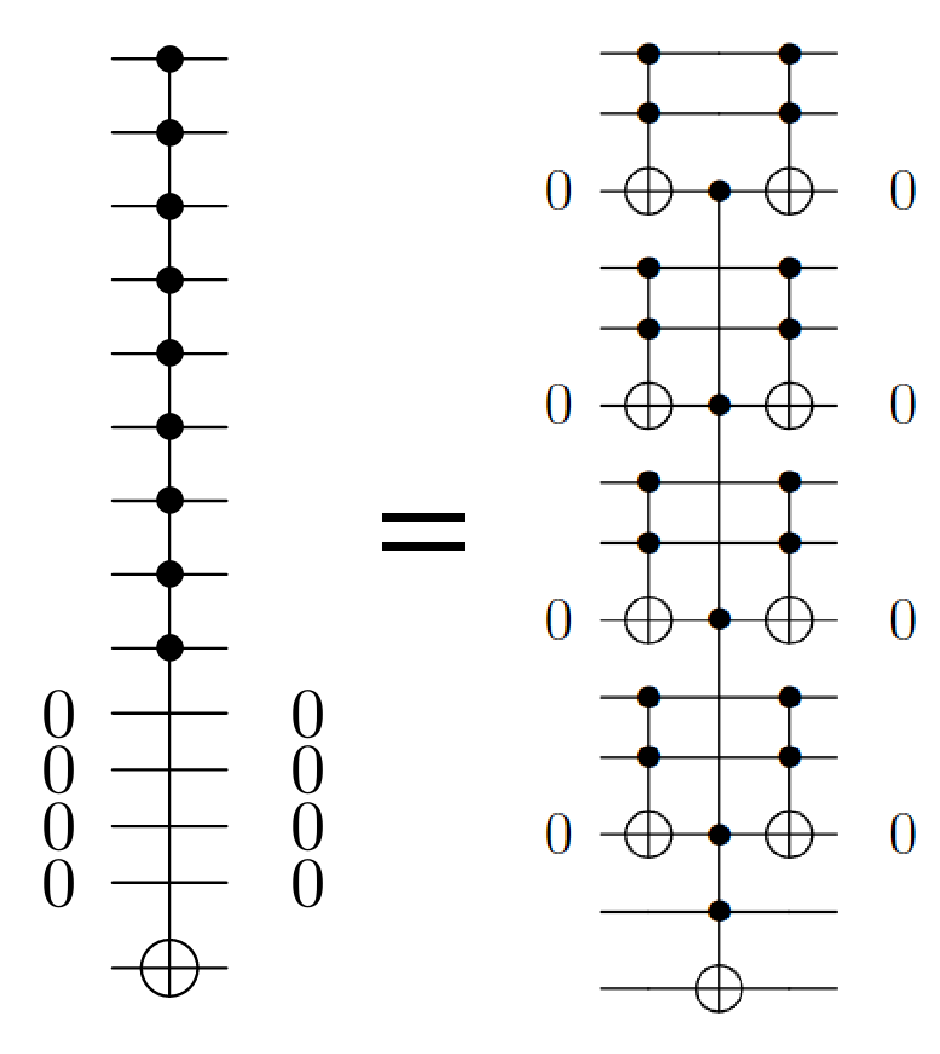
\includegraphics[width=8cm]{img/niemann_k_frac_c_2.pdf}
  \caption{4つの値が0の補助ビットを用いた$c=9$のMCTゲートの分解例}
  \label{niemann_frac_c_2}
\end{figure}
\subsection*{$\frac{c}{2} \bout{<} k \leq c-2$の場合}
\mout{$k>\frac{c}{2}$の場合では,
まず,$\lfloor\frac{c}{2}\rfloor$個の値が0の補助ビットを用いて,
1,3段目のすべてのMCTゲートをコントロールビット数が2となるよう分解する.
この際,2段目のMCTゲートのコントロールビットの数は,$c'=c-\lfloor \frac{c}{2}\rfloor$となる.
また,残りの値が0の補助ビット数は$k'=k-\lfloor \frac{c}{2} \rfloor$となる.
この残りの$k'$個の値が0の補助ビットを用いて,
\rout{$k'\leq \frac{c'}{2}$のときと,$k' > \frac{c'}{2}$の時に場合分けして,
2段目のコントロールビット数が$c'$のMCTゲートを分解する.}}
\par
\mout{
$k=c-2$のとき,
図~\ref{niemann_c_2}に示すように,
分解した全てのMCTゲートのコントロールビット数が2となる.
このため,$c-2$個より多くの値が0の補助ビットを加えても,
これ以上コントロールビットを分割できない.}
\begin{figure}[tbp]
  \centering
  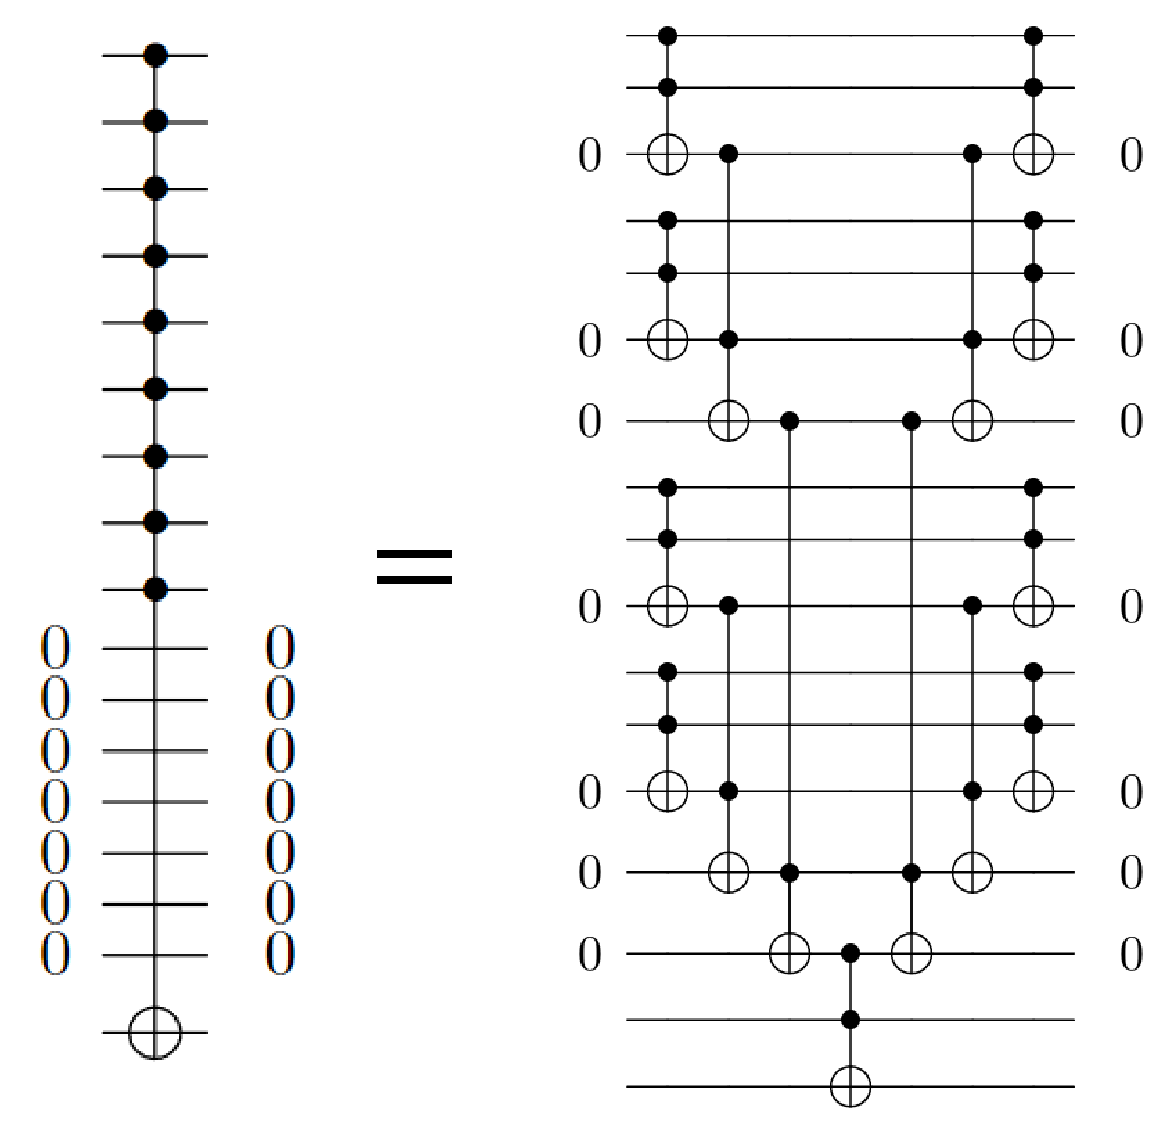
\includegraphics[width=9cm]{img/niemann_c_2.pdf}
  \caption{7つの値が0の補助ビットを用いた$c=9$のMCTゲートの分解例}
  \label{niemann_c_2}
\end{figure}
\chapter{ビットごとのT-depthを考慮したMCTゲートの分解手法}
本章では,提案手法である,ビットごとのT-depthを考慮したMCTゲートの分解手法について説明する.
\section{ビットごとのT-depth}
本節では,ビットごとのT-depthについて説明する.
ビットごとのT-depthとは,量子ビットごとにT-depthの値を計算したものである.
\par
ビットごとのT-depthの計算方法について説明する.
図~\ref{toffoli_bit}
にToffoliゲートの分解のビットごとのT-depthを示す.
各入力の量子ビットのビットごとのT-depthを$q_{x}, q_{y}, q_{z}$とする.
まず,図~\ref{toffoli_bit}の
左側の$T$ゲート実行後のT-depthは
その入力のビットごとのT-depthに1を足したものとなる.
図~\ref{toffoli_bit}の黒の実線で囲まれたCNOTゲートは,
入力のビットの実行が終わるまで実行できない.
このため,
黒の実線で囲まれたCNOTゲートの実行後の
ビットごとのT-depthは,入力のビットのビットごとのT-depthの最大値,
すなわち$\max\{q_{x}+1, q_{y}+1\}$と考えることができる.
赤の点線で囲まれたCNOTゲートに関しても同様に考えると,
実行後のビットごとのT-depthは,$\max\{q_{x}+1, q_{y}+1, q_{z}+1\}$となる.
このようにして,
Toffoliゲートの左側から順番にビットごとのT-depthを計算すると,
Toffoliゲート実行後のビットごとのT-depthは,$\max\{q_{x},q_{y},q_{z}\}+3$と考えることができる.
\begin{figure}
  \centering
  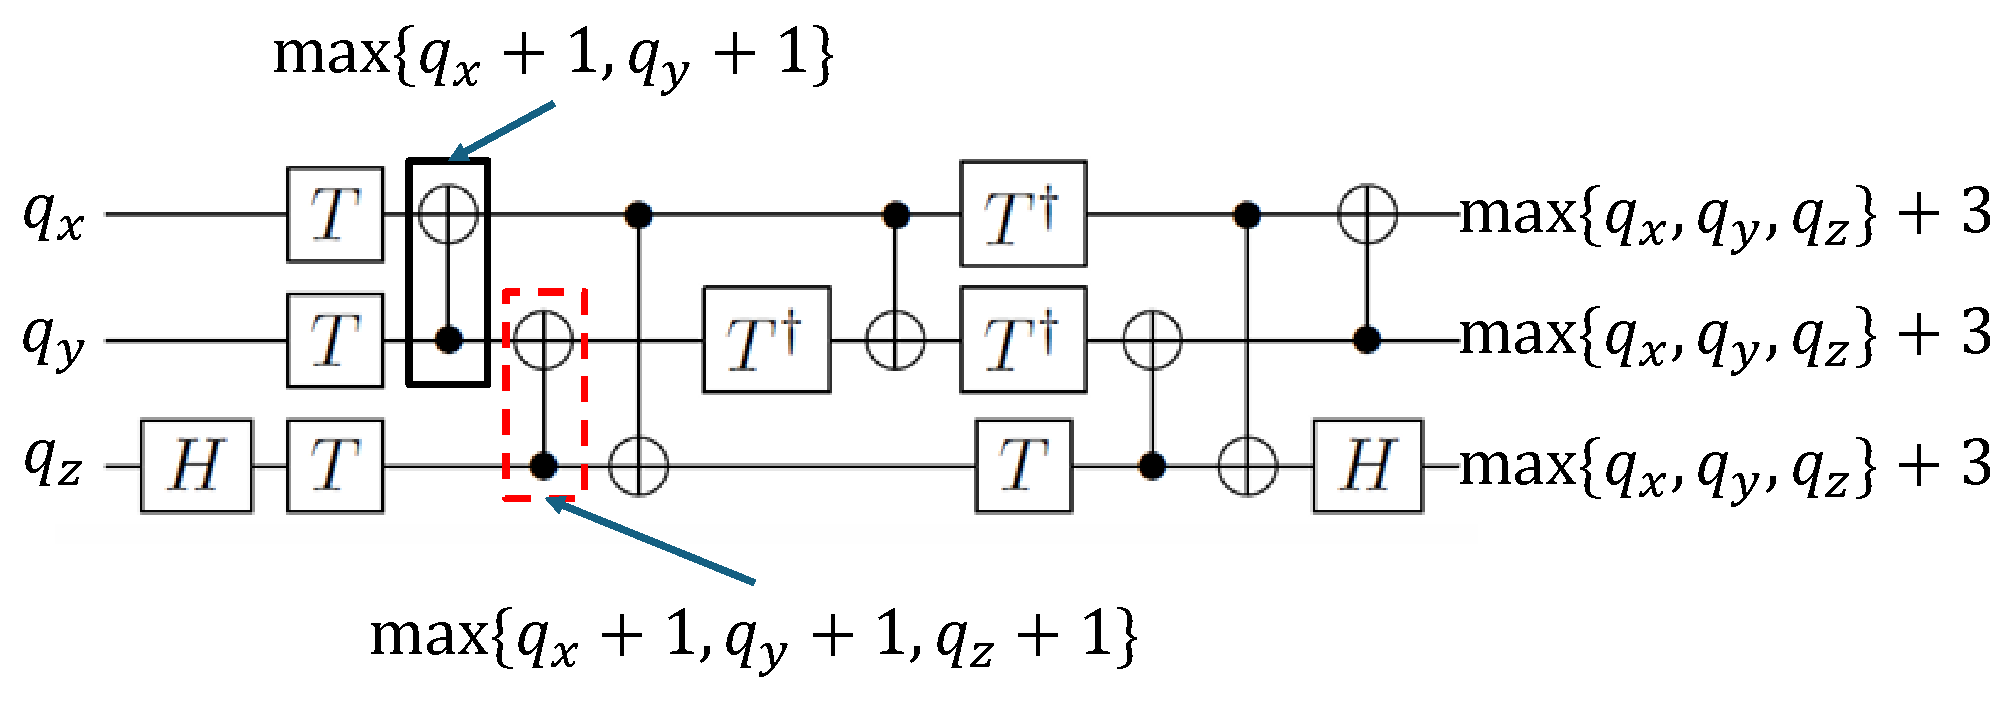
\includegraphics[width=12cm]{img/toffoli_bit.pdf}
  \caption{ToffoliゲートのビットごとのT-depth}
  \label{toffoli_bit}
\end{figure}
\par
ビットごとのT-depthは補助ビットを用いずにClifford+Tに,
分解できるゲートから計算を行うことができる.
表~\ref{tab:gate_tdepth}に補助ビットを用いずに
Clifford+Tに分解できるゲートを実行後のT-depthを示す.
表~\ref{tab:gate_tdepth}に基づき,
回路の左側からビットごとのT-depthを計算することで,
その回路のビットごとのT-depthを求めることができる.
\begin{table}[tbp]
  \centering
  \caption{補助ビットを用いずClifforf+Tに分解できるゲートの実行後のT-depth}
  \label{tab:gate_tdepth}
  \begin{tabular}{c|cc}
    ゲート名                         &使用量子ビット      &実行後のT-depth              \\ \hline
    $T, T^{\dag}$                    &$q_{x}       $      &$q_{x}+1$                    \\
    $H, NOT$                         &$q_{x}$             &$q_{x}$                      \\
    $CNOT$                           &$q_{x}, q_{y}$      &$\max\{q_{x}, q_{y}\}$       \\ 
    \bout{Toffoli}                   &$q_{x}, q_{y}, q_{z}$&$\max\{q_{x},q_{y},q_{z}\}+3$\\
    $CCiZ, CCiZ^{\dag}              $&$q_{x}, q_{y}, q_{z}$&$\max\{q_{x},q_{y},q_{z}\}+2$\\
    $CCi\omega Z, CCi\omega Z^{\dag}$&$q_{x}, q_{y}, q_{z}$&$\max\{q_{x},q_{y},q_{z}\}+1$\\
    $C\omega S, C\omega S^{\dag}$    &$q_{x}, q_{y}       $&$\max\{q_{x},q_{y}\}+1      $\\
  \end{tabular} 
\end{table}
\par
図~\ref{bit_tdepth}に
表~\ref{tab:gate_tdepth}に基づいてビットごとのT-depthを計算した例を示す.
図~\ref{bit_tdepth}の入力のビットごとのT-depthはすべて0とする.
図~\ref{bit_tdepth}の最大のT-depthは12であり,
最小のT-depthは8である.
図~\ref{bit_tdepth}は,
手法~1でコントロールビット数が4のMCTゲートを分解したものの,ビットごとのT-depthを求めたものである.
このようにビットごとのT-depthを計算すると,各ビットのT-depthに差が生じる.
このため,T-depthが小さいビットを優先して使用して,
\rout{MCTゲートを分解することで,}\bout{回路全体の}T-depthを削減することができる.
\begin{figure}
  \centering
  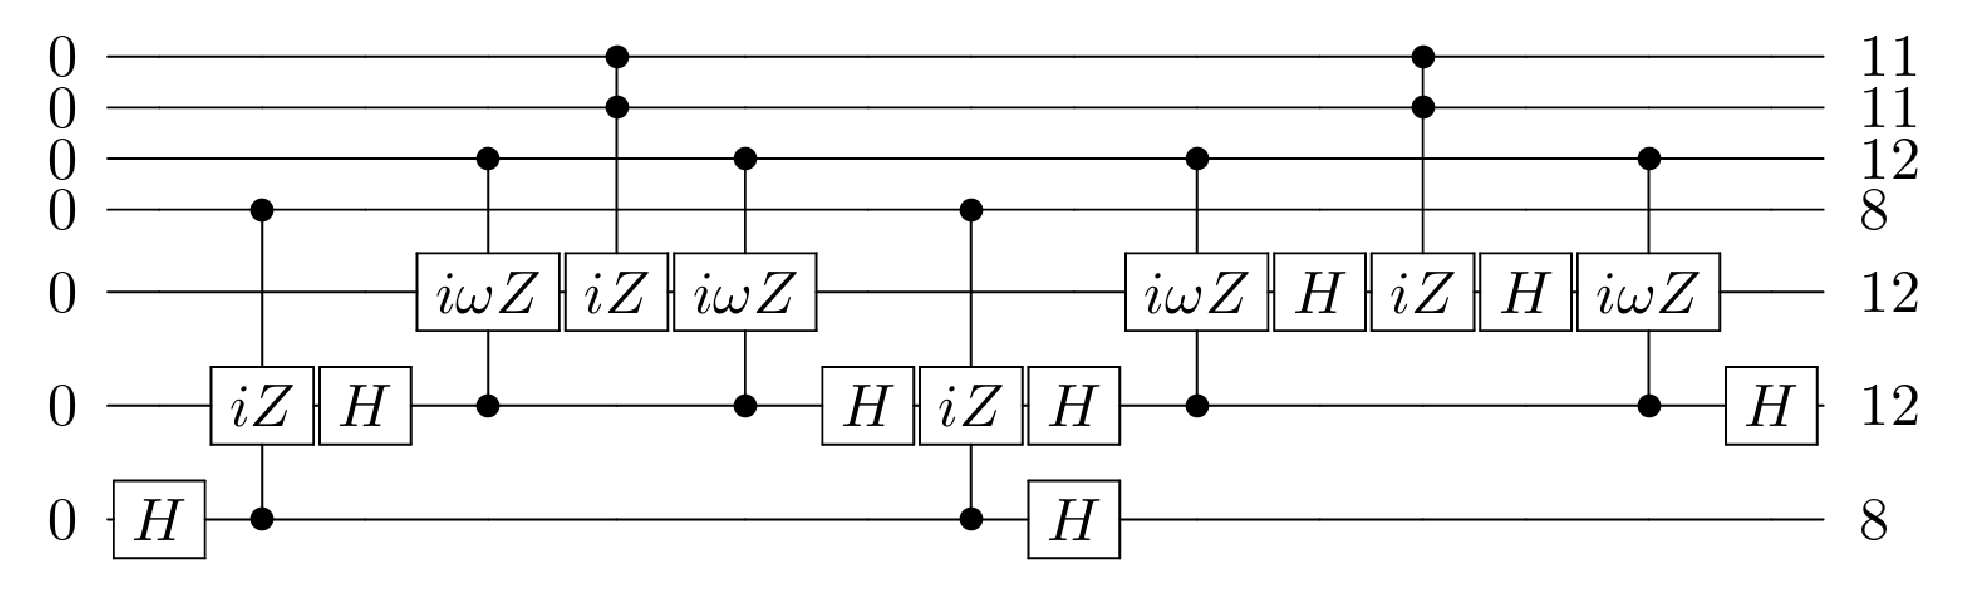
\includegraphics[width=14cm]{img/bit_tdepth.pdf}
  \caption{図~\ref{techmap}の回路のビットごとのT-depth}
  \label{bit_tdepth}
\end{figure}
\par
図~\ref{consider_tdepth}に
コントロールビット数が3個の
MCTゲートをビットごとのT-depthを\rout{考慮して分解した例}を示す.
図~\ref{consider_tdepth}では,入力側の各ビットのT-depthに差が生じている.
そのため,手法~1にビットのT-depthを考慮した分解を適用する場合,
使用するビットのT-depthが小さい順に使用することでT-depthを削減することができる.
図~\ref{bad_consider_tdepth}にビットの選択により分解後の最大のT-depthが悪化する例を示す.
図~\ref{bad_consider_tdepth}の例では,
はじめのゲート$g_{1}$に$q_{4}$のビットを使用した場合,
\bout{後続}のゲートの実行後のT-depthはその値に依存するため,最大のT-depthが20となる.
一方,図~\ref{consider_tdepth}では,
コントロールビットと補助ビットのT-depthが小さい順に使用することで,
分解後のビットのT-depthの最大値を削減している.
\begin{figure}[tbp]
  \centering
  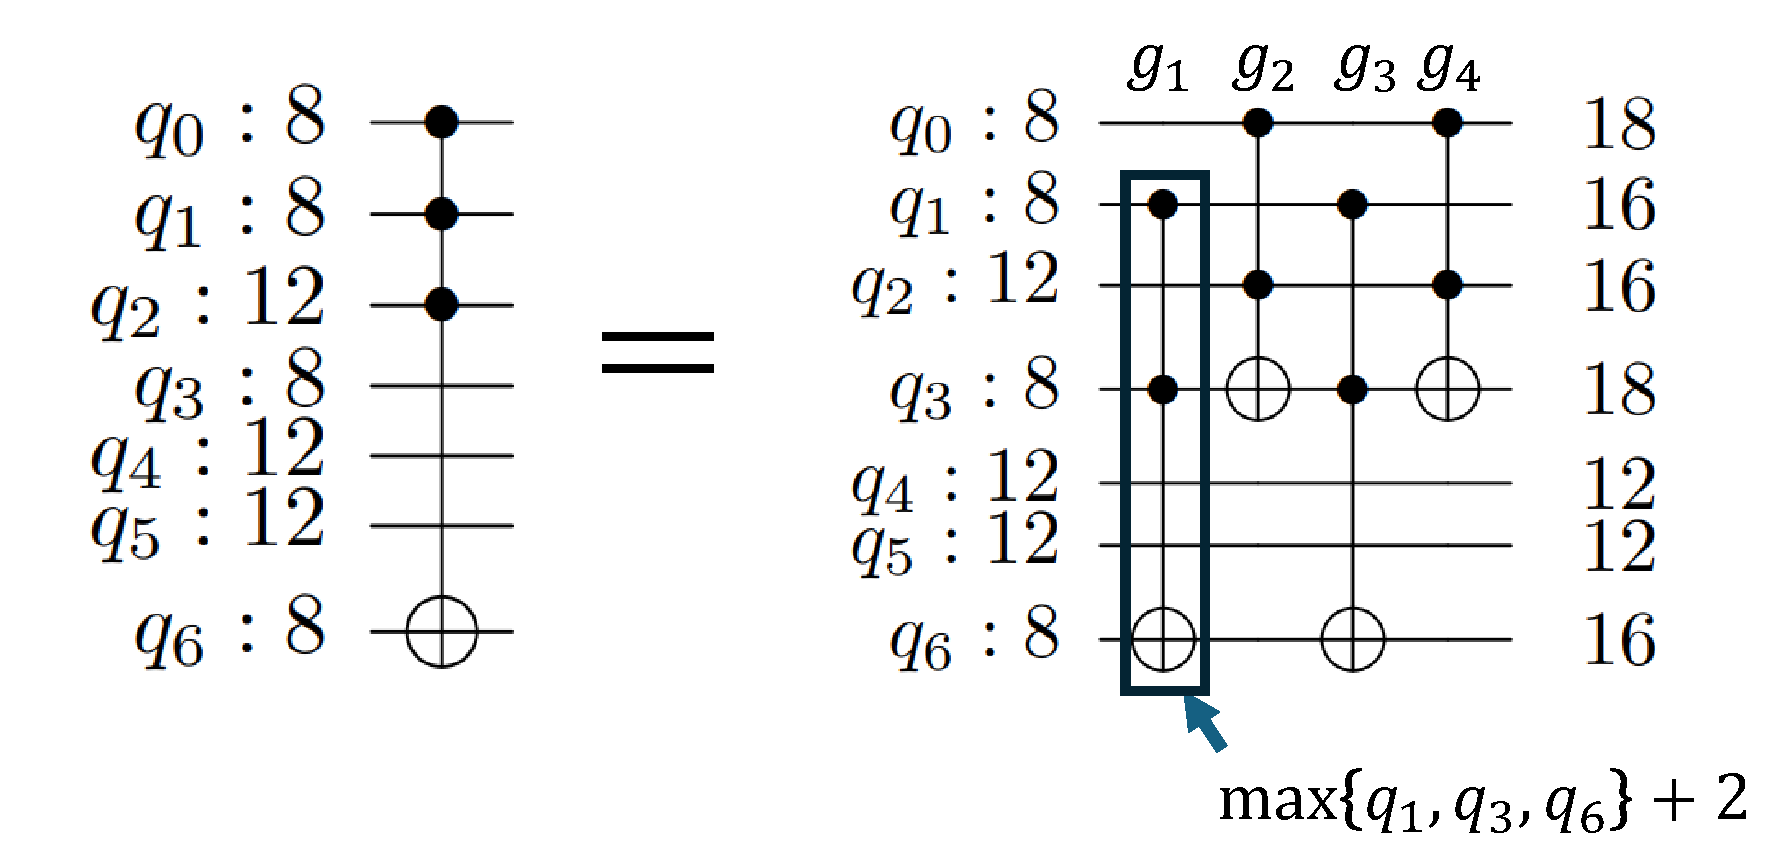
\includegraphics[width=10cm]{img/considering_bit_tdepth.pdf}
  \caption{コントロールビット数が3のMCTゲートをビットごとのT-depthを考慮し分解した例}
  \label{consider_tdepth}
\end{figure}
\begin{figure}[tbp]
  \centering
  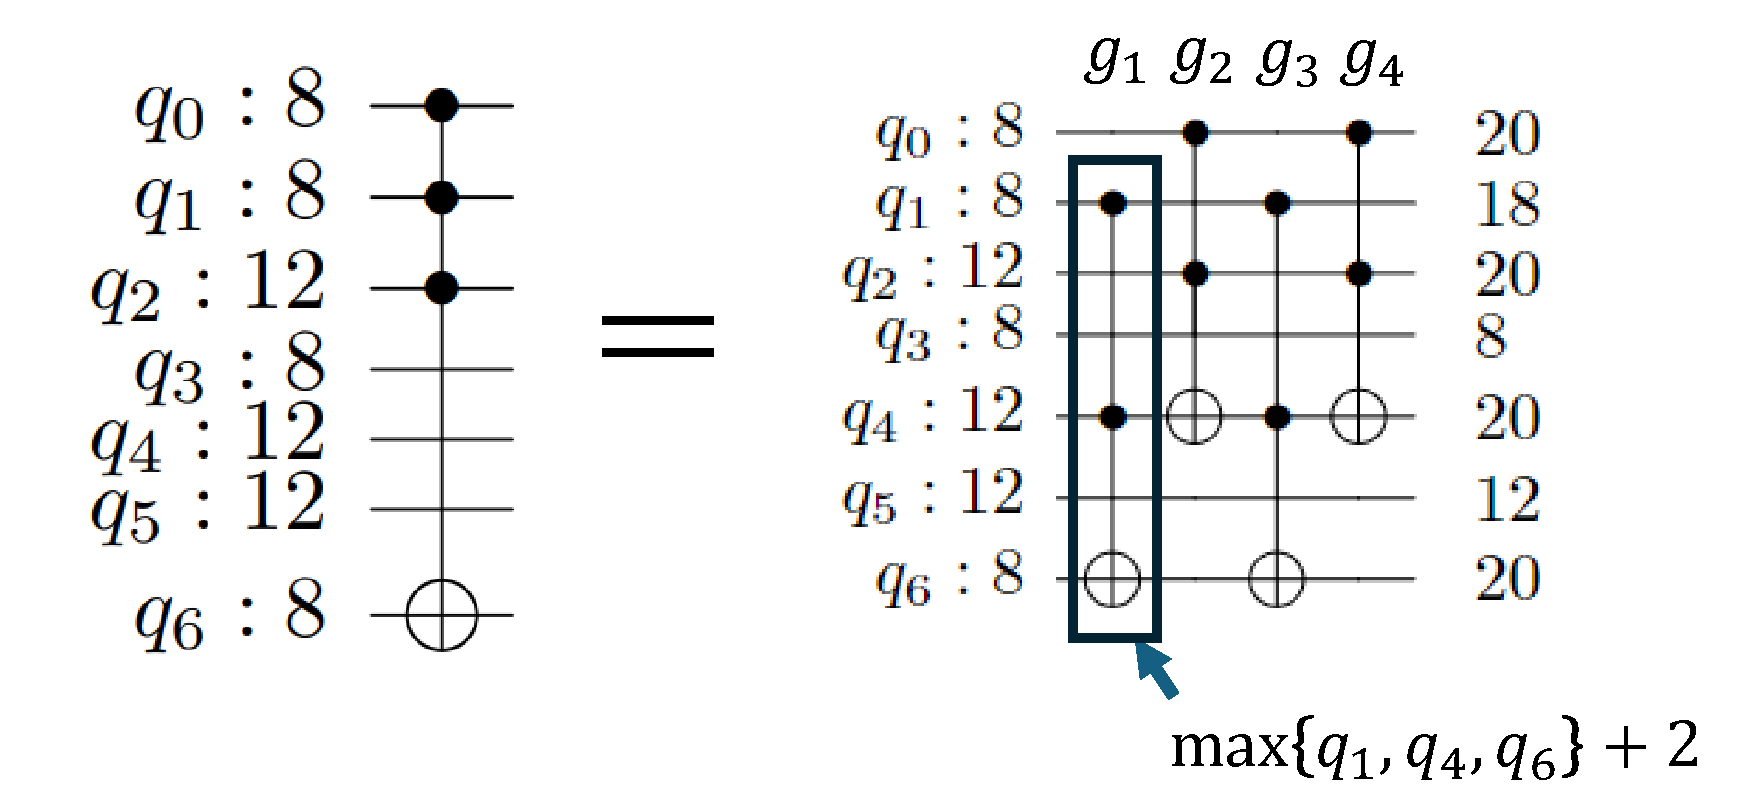
\includegraphics[width=10cm]{img/bad_consider_t-depth.pdf}
  \caption{コントロールビット数が3個のMCTゲートを分解した際に最大のT-depthが悪化する例}
  \label{bad_consider_tdepth}
\end{figure}
\section{ビットごとのT-depthを考慮したMCTゲートの分解}
本節では,
ビットごとのT-depthを考慮した,
MCTゲートの分解について手法1~4に適応\bout{した}方法を説明する.
ここで,分解前のMCTゲートの$c$個のコントロールビットの集合を$C$,
ターゲットビットを$t$とする.
\subsection{手法~1}
本項では,手法~1にビットごとのT-depth
を考慮した分解を適用する方法について説明する.
\par
手法1は,コントロールビットの数が3個以上の
MCTゲートをToffoliゲートに分解した後,
Toffoliゲートを$CCiZ, CCi\omega Z$ゲートに置換する手法である.
そのため,MCTゲートをToffoliゲートに分解する際に,
ゲートの配置が決定する.
\par
MCTゲートをToffoliゲートに分解する際のビットの選択方法について説明する.
図~\ref{barenco}の左から3個分のToffoliゲート\rout{$g_{1},g_{2},g_{3}$}
を構成するビットの配置が決定すれば,
その右側のゲートはこれらのゲートの複製であるため,\bout{MCTゲートの}分解が決定する.
すなわち,
$c-2$個の値が不定の補助ビットを用いてMCTゲートを分解する手法~\cite{barenco1995elementary}では,
$c-1$個のToffoliゲートの配置を決定することで,分解を実現できる.
これらのゲートを構成するビットの決定方法を説明する.
\par
分解前のMCTゲートのコントロールビットを
T-depthが小さい順に並び変えたものを$c_{1},\dots, c_{c}$とする.
分解前のMCTゲートのターゲットビットを$t$とする.
分解後の左から$c-1$個のToffoliゲートを$g_{1},\dots ,g_{c-1}$とする.
$g_{1},\dots, g_{c-1}$の
コントロールビットの集合を$C_{1},\dots, C_{c-1}$とする.
$c-2$個の値が不定の補助ビットをT-depthの小さい順に並び変えたものを,
$a_{1},\dots ,a_{c-2}$とする.
$g_{1},\dots ,g_{c-1}$の構成するビットの決定方法を以下に示す.
\begin{enumerate}[手順1]
  \item $C_{1}\dots, C_{c-2}$に$a_{1},\dots, a_{c-2}$をそれぞれ順番に1つずつ追加する.
  \item $C_{1},\dots ,C_{c-2}$に順番に$c_{1},\dots ,c_{c-2}$を追加する.
  \item $C_{c-1}$に$c_{c-1}, c_{c}$を追加する.
  \item $g_{1}$のターゲットビットを$t$とする.
  \item $g_{2},\dots, g_{c-2}$のターゲットビットをそれぞれ順番\rout{に}$a_{1}, \dots , a_{c-2}$とする.
\end{enumerate}
\par
上記の手順に則り,$g_{1},\dots ,g_{c-1}$を構成するビットを決定した\rout{後,}
式~\ref{eq:toffoli_haiti}の順番に回路の左側からToffoliゲートを配置する.
\begin{equation}\label{eq:toffoli_haiti}
  \{g_{1}, g_{2}, \dots g_{c-1}\}, \{g_{c-2},g_{c-3},\dots g_{1}\}, \{g_{2},g_{3},\dots ,g_{c-1}\}, \{g_{c-2}, g_{c-3}\dots ,g_{2}\}
\end{equation}
最後に,配置したこれらのゲートを手法~1により,$CCiZ, CCi\omega Z$ゲートに置換する.
このように,T-depthの小さいビットを順番に左側のToffoliゲートから配置することで,
T-depthの大きなビットをはじめに使うことを防ぐことができる.
\par
\bout{図~\ref{b2mapping_proposed}はビットごとのT-depthを考慮し,
コントロールビット数が4個のMCTゲートを手法~1で分解した例を示す.
図~\ref{b2mapping_proposed}の左側の分解前のMCTゲートのコントロールビットをT-depthが小さい順に並び変えると,
$C=\{c_{3}, c_{2}, c_{4}, c_{1}\}$である.
値が不定の補助ビットは$a_{1},a_{2}$の順でT-depthが小さい.
まず,$g_{1}, g_{2}, g_{3}$を構成するビットを決定する.
$g_{1}$のコントロールビットを,T-depthが小さい順に選択すると$c_{3}, a_{1}$となり,
ターゲットビットは$t$である.
次に,$g_{2}$のコントロールビットを,
T-depthが小さい順に選択すると,$c_{2}, a_{2}$となり,
ターゲットビットは,$a_{1}$となる.
最後に$g_{3}$のコントロールビットは$c_{4},c_{1}$となり,
ターゲットビットは$a_{2}$となる.
このようにして,$g_{1},g_{2},g_{3}$を構成するビットを決定し,
式~\ref{eq:toffoli_haiti}の順でToffoliゲートを配置する.
配置したToffoliゲートを,手法~1により,$CCiZ, CCi\omega Z$ゲートに置換すると,
図~\ref{b2mapping_proposed}の右側のようになる.この時のT-depthの最大値は,24となる.}
\begin{figure}
  \centering
  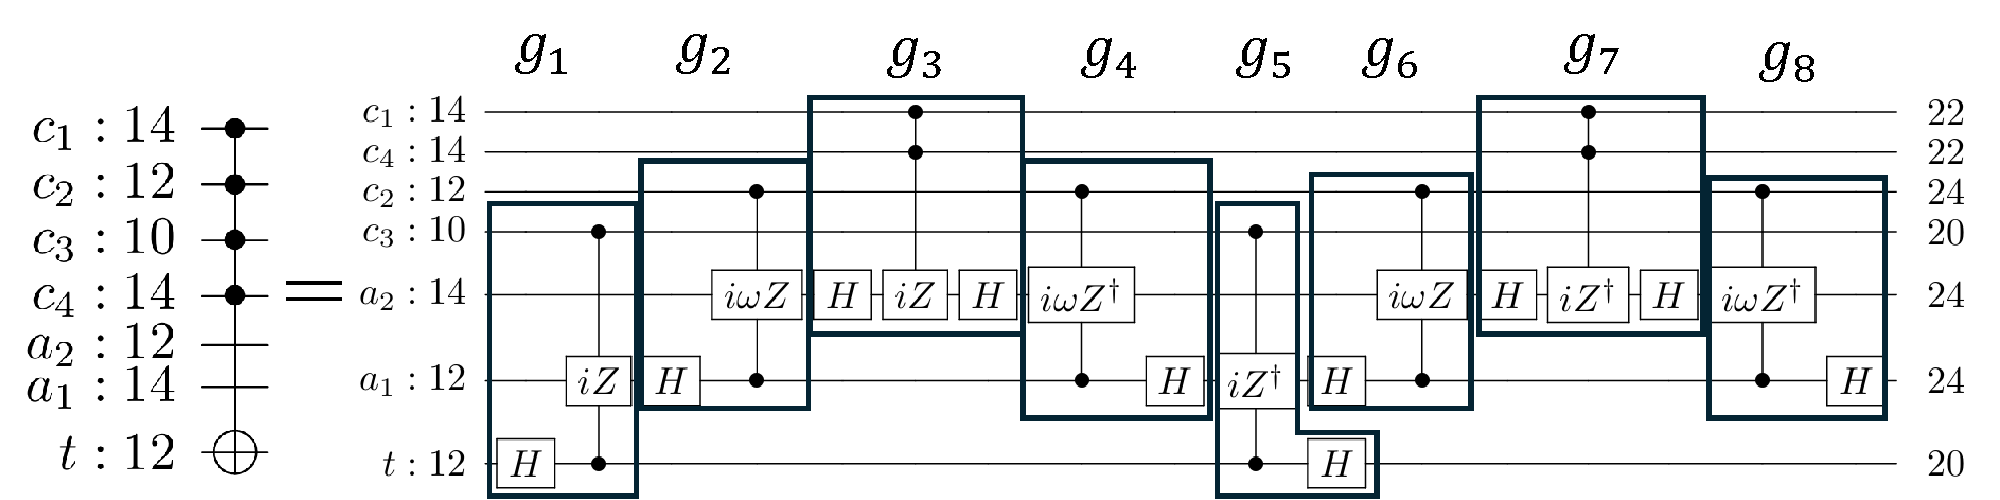
\includegraphics[width=18cm]{img/b2_mapping_proposed.pdf}
  \caption{コントロールビット数が4個のMCTゲートをビットごとのT-depthを考慮し手法1で分解した例}
  \label{b2mapping_proposed}
\end{figure}

\begin{comment}
\begin{algorithm}[tbp]
  \caption{ビットごとのT-depthを考慮した分解}\label{alg:b2map_bit}
  \begin{algorithmic}[1]
    \Require $tdepth\Leftarrow$ 各量子ビットごとのT-depth
    \Require $C\Leftarrow$ 分解するMCTゲートのコントロールビットのリスト
    \Require $t\Leftarrow$ 分解するMCTゲートのターゲットビット
    \Require $D\Leftarrow$ 初期化されていない補助ビットのリスト
    \Ensure $circ$: 分解済みのMCTゲート
    \State $C \Leftarrow$ コントロールビットのリストをT-depthが小さい順にソート
    \State $D \Leftarrow$ 補助ビットのリストをT-depthが小さい順にソート
    \For{$(q,index) \leftarrow $Cの要素とそのindex}
    \If{$i==0$}
      \State 
    \EndIf
    \EndFor
  \end{algorithmic}
\end{algorithm}
\end{comment}
\subsection{手法2}
本項では,ビットごとのT-depthを考慮した分解を手法~2に適用する方法を説明する.
\par
手法~2では,MCTゲートを4つの$C\omega S$ゲートと4つのMCTゲートに分解する.
まず,分解で現れる4つの$C\omega S$ゲートと4つのMCTゲートを構成するビットの決定方法について
説明する.
1つの値が不定のビットを$a$とする.
まず,4つの$C\omega S$ゲートは1つの値が不定の補助ビット$a$をコントロールビットに持ち,
ターゲットビットに$t$をもつ.
次に,分解で現れる4つのMCTゲートは左側から,$g_{1},\dots, g_{4}$とする.
$g_{1}, g_{2}$を構成するビットの決定方法について説明する.
$g_{1}, g_{2}$のコントロールビットの集合を$C_{1}, C_{2}$とする.
分解前のMCTゲートの$c$個のコントロールビットを,
T-depthが小さい順にソートしたものを$c_{1},\dots, c_{c}$とする.
式~\ref{eq:method2bunkatu}の通りに$C_{1}, C_{2}$を決定する.
\begin{equation}\label{eq:method2bunkatu}
  C_{1}=\{c_{1},\dots, c_{\lfloor c/2 \rfloor}\}, C_{2}=\{c_{\lfloor c/2 \rfloor +1},\dots , c_{c}\}
\end{equation}
$g_{1}, g_{2}$のターゲットビットは$a$である.
$g_{3}, g_{4}$についてはそれぞれ,$g_{1}$, $g_{2}$の複製であるため,
これらのゲートと同じビットで構成される.
このようにして,
分解で現れる4つの$C\omega S$ゲートと4つのMCTゲートを構成するビットを決定する.
\par
分解で現れる4つの$C\omega S$ゲートと
4つのMCTゲートを構成するビットを決定した後,
これらのゲートを左側から順番に分解して,ビットごとのT-depthの更新を繰り返す.
Algorithm~\ref{alg:method2_placement_decomp}に従い,これらのゲートを分解,配置する.
このように,左側のゲートから分解することで,
各ゲートをビットごとのT-depthを考慮し,\bout{MCTゲートを}分解できる.
\begin{algorithm}[tbp]
  \caption{ビットごとのT-depthを考慮した手法~2の分解と配置}
  \label{alg:method2_placement_decomp}
  \begin{algorithmic}[1]
    \Require MCTゲート$g_{1},\dots, g_{4}$
    \Require $C\omega S$ゲート
    \Require 各ビット$c_{1},\dots, c_{c}, a, t$とT-depthの対応
    \Ensure 補助ビットを用いずClifford+Tに分解できるゲートで構成される回路$OC$
    \State $g_{i}$のコントロールビットの集合$C_{i}$
    \For{i={1,\dots ,2}}
    \State $OC$に$C\omega S$ゲートを追加,各ビットのT-depthを更新
    \State $C_{(i+1)\% 2}$からT-depthの小さい順にビットを$|C_{i}|-2$個取り出す.
    \State 取り出した$|C_{i}-2|$個のビットを補助ビットとして$g_{i}$をビットごとのT-depthを考慮し手法~1により分解.
    \State $g_{i}$の分解結果を$OC$に追加,各ビットのT-depthを更新
    \EndFor
    \For{i={1,\dots ,2}}
    \State $OC$に$C\omega S$ゲートを追加する.
    \State $OC$に$g_{i}$の分解を逆変換のゲートに置換した上で逆順にしたものを追加する.
    \EndFor
  \end{algorithmic}
\end{algorithm}
\par
\begin{figure}
  \centering
  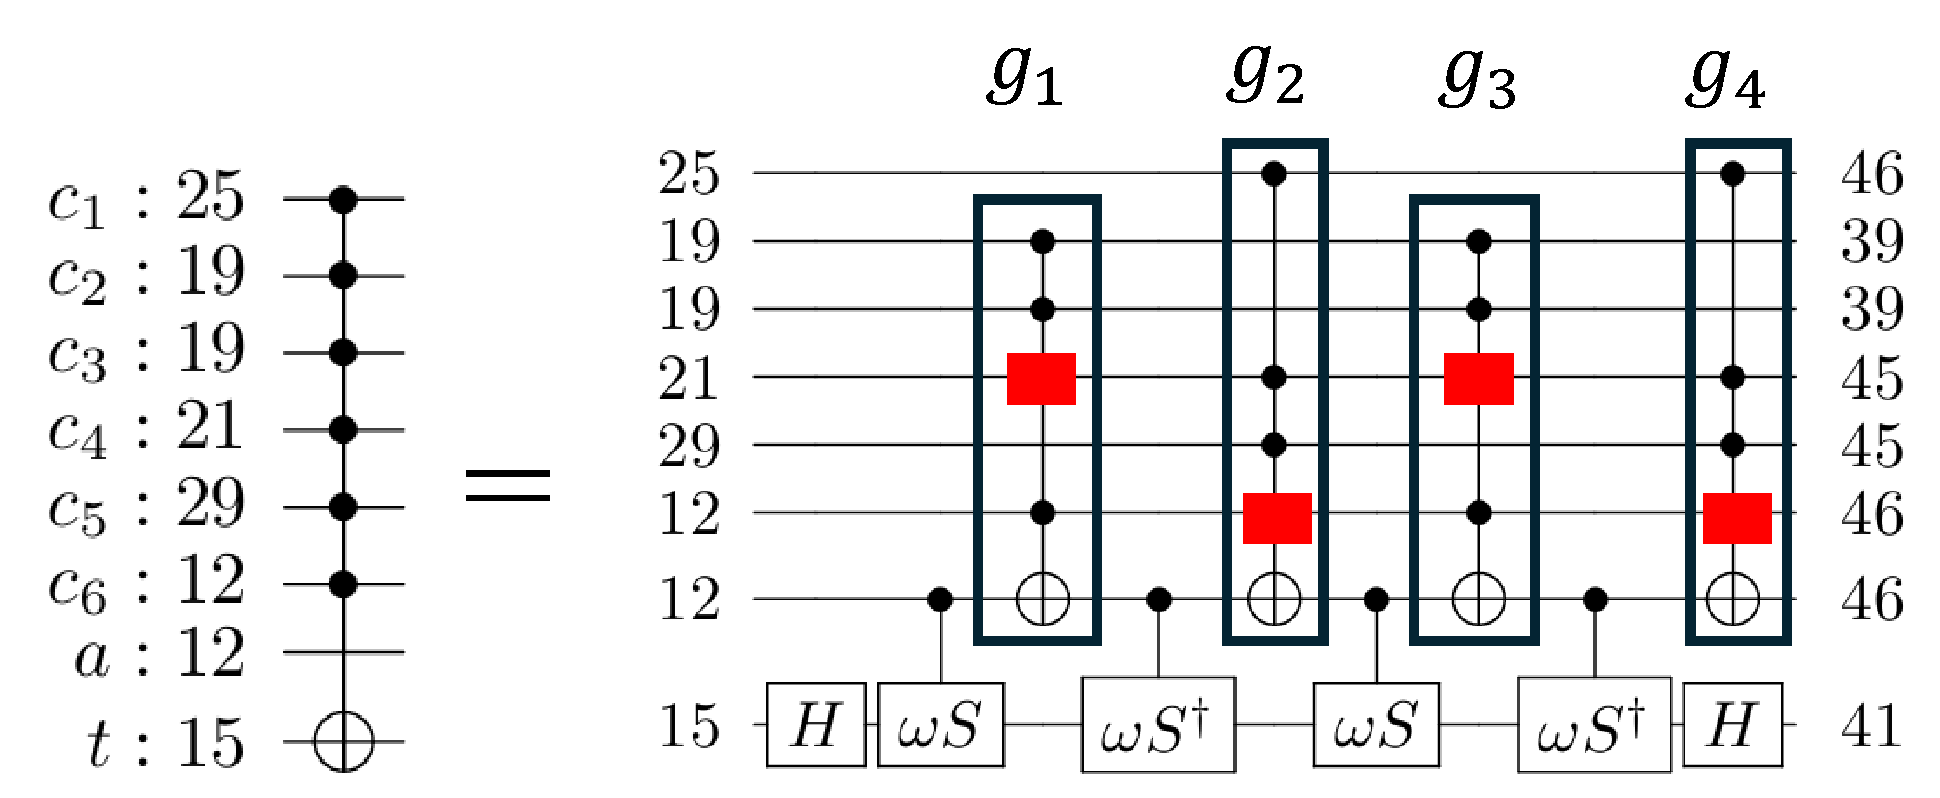
\includegraphics[width=10cm]{img/mimap_proposed.pdf}
  \caption{コントロールビット数が6個のMCTゲートをビットごとのT-depthを考慮し,手法~2を用いて分解した例}
  \label{mimap_proposed}
\end{figure}
\bout{図~\ref{mimap_proposed}にビットごとのT-depthを考慮し,
手法~2を用いて$c=6$のMCTゲートを4つのMCTゲートと,
4つの$C\omega S$ゲートに分解した例を示す.
まず,ビットごとのT-depthを考慮して,手法~2を用いてMCTゲートを分解するには,
式~\ref{eq:method2bunkatu}に従い,コントロールビットをT-depthの小さい順に2つの集合に分割する.
図~\ref{mimap_proposed}の例では,$C_{1}=\{c_{6}, c_{2},c_{3}\}, C_{2}=\{c_{1}, c_{4}, c_{5}\}$となる.
コントロールビットの分割を決定すると,
4つのMCTゲートと,$C\omega S$ゲートの構成するビットを決定できる.
図~\ref{mimap_proposed}の右側が,
$c=6$のMCTゲートを4つのMCTゲートと,
4つの$C\omega S$ゲートに分解した例である.}
\par
\bout{最後に,図~\ref{mimap_proposed}の右側の回路のゲートをAlgorithm~\ref{alg:method2_placement_decomp}
に従い分解する.
まず,$g_{1}$までのゲートの分解結果から各ビットのT-depthを計算し,
$c_{3}$を補助ビットとして用いて,$g_{1}$を分解する.
次に,$g_{2}$までのゲートの分解結果から,$c_{6}$を補助ビットとして用いて$g_{2}$を分解する.
最後に$g_{3}, g_{4}$は,それぞれ$g_{1}, g_{2}$の分解を逆変換に置換した上で,逆順にして配置する.
このようにして,各ゲートを分解することで,
図~\ref{mimap_proposed}の分解結果の最大のT-depthは46となる.}
\subsection{手法3}
手法~3にビットごとのT-depthを考慮した分解を適用する方法について説明する.
\par
手法~3では,分解に使用する値が不定の補助ビットの数$m\geq 2$と,
分解するMCTゲートのコントロールビット数$c$に応じて,
分解後の各MCTゲートのコントロールビット\rout{数を決定する.}
手法~3により求めた,
分解後の各MCTゲート$g_{1},\dots, g_{m+1}$の
コントロールビット数を$N_{1},\dots, N_{m+1}$とする.
ここで,手法~3では,
$1$番目と,$m+1$番目のゲートにコントロールビットを優先的に配置するため,
$N_{2},\dots, N_{m}$の値は2である.
\par
まず,手法~3の分解を決定するには,$g_{1},\dots ,g_{m+1}$の配置を決定する必要がある.
しかし,
$g_{1}$のコントロールビット数が3個以上であると,
$g_{1}$の分解の結果に応じて,$g_{2},\dots, g_{m+1}$で使用するビットのT-depthが変化する.
そのため,あらかじめ$g_{1}$をビットごとのT-depthを考慮し分解した上で,
その結果に応じて,$g_{2},\dots, g_{m+1}$の配置を決定する必要がある.
$g_{1},\dots,g_{m+1}$のコントロールビットの集合を$C_{1},\dots, C_{m+1}$とする.
分解に使用する値が$m$個の不定のビットの集合を$A$とする.
以下の手順に則り,$g_{1},\dots ,g_{m+1}$の配置を決定する.
\begin{enumerate}[手順1]
  \item $g_{1}$の配置を決定し,分解する.分解の結果から各ビットのT-depthを更新
  \begin{enumerate}
    \item $C_{1}$に$A$から,T-depthが最小の要素を移動する.
    \item $|C_{1}|=N_{1}$となるよう,$C$からT-depthが小さい順に要素を移動する.
    \item $t_{1}=t$とする.
    \item $C_{1}$と$t$でないビットのうちT-depthが小さい順に$|C_{1}|-2$個ビットを選択する.
    \item 選択したビットを補助ビットとして,ビットごとのT-depthを考慮し,手法~1で$g_{1}$を分解する.
    \item 分解の結果から,各ビットのT-depthを更新する.
  \end{enumerate}
  \item $g_{2}, \dots ,g_{m+1}$をT-depthが小さい順にビットを選択し,配置する.
  \begin{enumerate}[(1)]
    \item $i=2$とする.
    \item $C_{i}$に$A$のうち,T-depthが最小の要素を移動する.
    \item $|C_{i}|=N_{i}$となるよう,$C$からT-depthが小さい順に要素を移動する.
    \item $t_{i}$を$g_{i-1}$に移動した$A$の要素とする.
    \item $i < m+1$である限り,$i=i+1$とし,(2)に戻る.そうでなければ,終了する.
  \end{enumerate}
 \end{enumerate}
 このような手順で$g_{1},\dots ,g_{m+1}$の配置を決定する.
 その後,
 Algorithm~\ref{alg:method3_placement_decomp}に従い,
 分解とビットごとのT-depthの更新を繰り返し,
 数式~\ref{eq:bakerhaiti}の順番で並ぶMCTゲートを分解,配置する.
 \begin{algorithm}[tbp]
  \caption{ビットごとのT-depthを考慮した手法~3の配置と分解}
  \label{alg:method3_placement_decomp}
  \begin{algorithmic}[1]
    \Require 数式~\ref{eq:bakerhaiti}のMCTゲートのリスト:$mctlist$
    \Require 各ビットとT-depthの対応
    \Ensure 補助ビットを用いずClifford+Tに分解できるゲートで構成される回路:$OC$
    \ForEach{$g \leftarrow mctlist$}
    \State $g$で使用していないビットの集合:$A$
    \State $g$のコントロールビット数:$c$
    \State $A$からT-depthの小さい順にビットを$c-2$個取り出す.
    \State 取り出した$c-2$個のビットを補助ビットとして$g$をビットごとのT-depthを考慮し手法~1により分解
    \State $g$の分解結果を$OC$に追加,各ビットのT-depthを更新
    \EndFor
  \end{algorithmic}
\end{algorithm}
\par
\bout{図~\ref{baker_proposed}に,ビットごとのT-depthを考慮した手法~3により,$c=5$のMCTゲートを分解した例を示す.
図~\ref{baker_proposed}の分解について説明する.
まず,
手法~3を用いて,
図~\ref{baker_proposed}の左側のゲートを分解したときの,
各ゲートのコントロールビット数を求めると,
$N_{1}=3, N_{2}=2, N_{3}=2$となる.
次に,$g_{1}, g_{2}, g_{3}$を構成するビットを順に決定する.
まず,$g_{1}$のコントロールビット$C_{1}$を決定する.
補助ビット$a_{1}, a_{2}$のうち,T-depthが最小のビット$a_{2}$を$C_{1}$に移動する.
また,$c_{1},\dots,c_{5}$から,T-depthの値が小さい順に2つのビット,$c_{2}, c_{5}$を選択し,$C_{1}$に移動する.
$g_{1}$のターゲットビットを$t$とする.
$g_{1}$はコントロールビット数が3なので,$g_{1}$の分解結果により,後続のゲートを構成するビットが変化する.
そのため,$g_{1}$が使用していないビットから,T-depthが小さい順に$|C_{1}|-2$個ビットを選択し,$g_{1}$を分解する.
図~\ref{baker_proposed}の例では,$c_{3}$を補助ビットとし,$g_{1}$を分解し,T-depthを再計算する.
再計算すると,各ビットのT-depthは,$c_{2}=27, c_{3}=27, c_{5}=27, a_{2}=25, t=25$となる.
この結果から,$g_{2}, g_{3}$を構成するビットを決定する.
$g_{2}$のコントロールビットは$a_{1}$と,
$c_{1}, c_{3}, c_{4}$のうち,T-depthが最小のビットである$c_{1}$となる.
また,$g_{2}$のターゲットビットは,$a_{2}$となる.
$g_{3}$のコントロールビットは残りのコントロールビット$c_{3}, c_{4}$となり,
ターゲットビットは,$a_{1}$となる.
このようにして,$g_{1}, g_{2}, g_{3}$を構成するビットを決定し,
式~\ref{eq:bakerhaiti}の順で配置することで,図~\ref{baker_proposed}の右側の分解を実現できる.}
\par
\bout{最後に図~\ref{baker_proposed}
の右側のゲート$g_{1},\dots, g_{8}$を
Algrorithm~\ref{alg:method3_placement_decomp}に従い,
左側から分解,配置することで,ビットごとのT-depthを考慮した,手法~3の分解を決定できる.
まず,$g_{1}$はT-depth最小の$c_{3}$を補助ビットとして用いて分解する.
$g_{5}$は,$g_{1},\dots, g_{4}$の分解結果から,T-depth最小のビット$c_{4}$を補助ビットとして用いて分解する.
すべてのゲートを分解した結果,最大のT-depthは41となる.}
\begin{figure}[tbp]
  \centering
  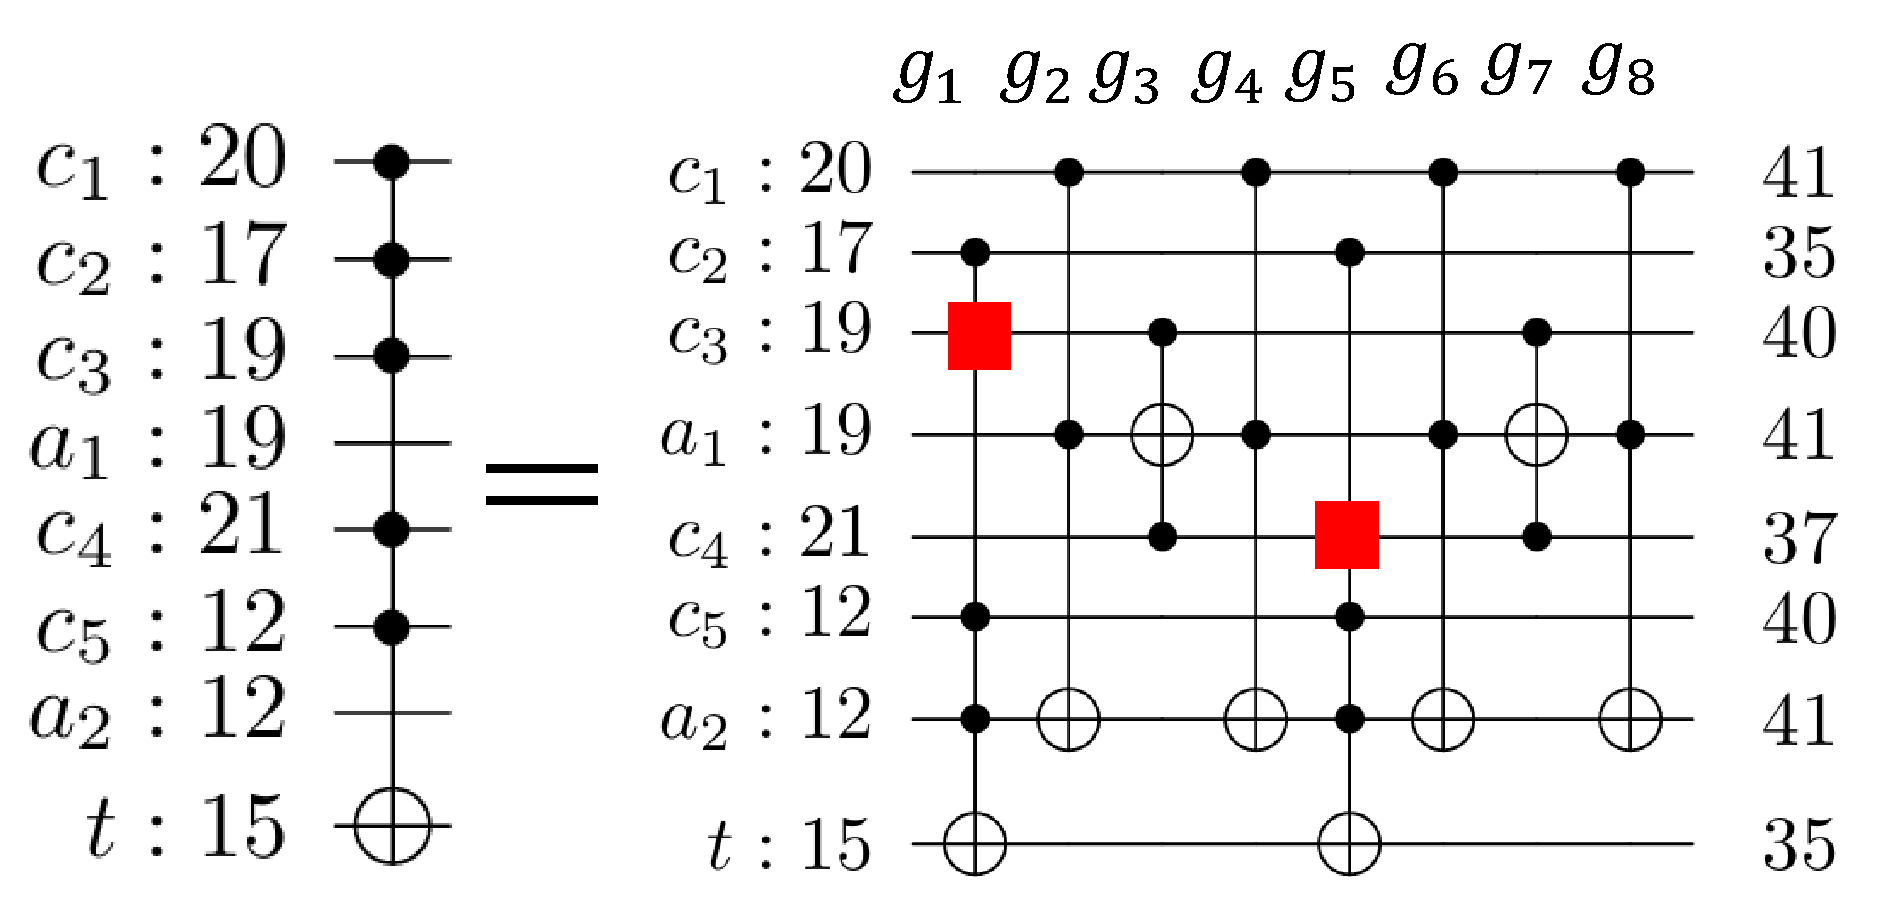
\includegraphics[width=10cm]{img/baker_proposed.pdf}
  \caption{2個の値が不定の補助ビットを用いて,ビットごとのT-depthを考慮し手法3を用いて,$c=5$のMCTゲートを分解した例}
  \label{baker_proposed}
\end{figure}
\begin{comment}
  \begin{algorithm}[tbp]
  \caption{ビットごとのT-depthを考慮した手法~3の配置と分解}
  \label{alg:method3_placement_decomp}
  \begin{algorithmic}[1]
    \Require 分解前のMCTゲート$(C, t)$ \Comment{$C$はコントロールビットの集合,$t$はターゲットビット}
    \Require $m$個の補助ビットのリスト$A$ 
    \Require 各ビットのT-depth
    \Ensure 補助ビットを用いずClifford+Tに分解できるゲートで構成される回路$OC$
    \State 空のビットのリスト$C_{1},\dots ,C_{m+1}$
    \State $m+1$個のビット$t_{1},\dots, t_{m+1}$
    \State $t_{1} \leftarrow t$
    \State $C_{1}$に$A$の内T-depthが最も小さいビットを追加
    \State $t_{2} \leftarrow A$の内T-depthが最も小さいビット
    \State $A$から最もT-depthが小さいビットを削除
    \State $C \leftarrow$ 分解前のMCTゲートのコントロールビット 
    \While{$|C_{1}|-2 \leq c+m-1$かつ$|C|\geq m$}
      \State $C_{1}$に$C$のT-depthが最も小さいビットを追加
      \State $C$の最もT-depthが小さいビットを削除
    \EndWhile
    \State $g_{1}\leftarrow (C_{1}, t_{1})$
    \State $g_{1}$を$g_{1}$を構成するビットでないビットのうち,$|C_{1}|-2$個のビットを使用し分解する
    \State $OC$に$g_{1}$の分解を追加
    \State 各ビットのT-depthを更新
    \For{$i={2,\dots ,m}$}
      \State $C_{i}$に$A$のT-depth最小の要素追加
      \State $t_{i+1}\leftarrow A$のT-depth最小の要素
      \State $A$からT-depth最小の要素を削除
      \State $C_{i}$に$C$のうち最もT-depthが小さな要素を追加
      \State $C$からT-depthが最も小さな要素を削除
      \State $g_{i}\leftarrow (C_{i}, t_{i})$
      \State $g_{i}$を$CCi\omega Z$ゲートに置換
      \State $OC$に$g_{i}$を追加
    \EndFor
    \State 各ビットのT-depthを更新
    \State $C_{m+1} \leftarrow C$
    \If{$|C_{m+1}|=2$}
    \State $g_{m+1}$を$CCiZ$ゲートに置換
    \State $g_{m+1}$を$OC$に追加
    \Else
    \State $g_{m+1}$を構成しないビットのうち,T-depthが小さい順に$|C_{m+1}|-2$個ビットを取り出す.
    \State 取り出したビットを補助ビットとして$g_{m+1}$をビットごとのT-depthを考慮し分解
    \EndIf
  \end{algorithmic}
\end{algorithm}
\end{comment}
\subsection{手法4}
手法4をビットごとのT-depthを考慮して分解する方法について説明する.
\par
手法4では,分解に使用する補助ビットの数に応じて,
複数段にMCTゲートを分解する.
分解した各MCTゲートのコントロールビット数は,
使用する補助ビットの数と,分解するMCTゲートのコントロールビット数に応じて,変化する.
分解に使用する値が不定の補助ビットの数を$d$,分解に使用する値が0の補助ビットの数を$k$とする.
これらの$c, k, d$の値により手法4から,
各段のMCTゲートのコントロールビット数が求められる.
手法4を用いて,
MCTゲートを分解したとき$n$段に分解できるとする.このとき,$n$は3以上の奇数である.
式~\ref{eq:niemann_cnt}のように,
2次元配列を用いて,求めた各段のMCTゲートのコントロールビット数を表すとする.
式~\ref{eq:niemann_cnt}では,
$n$段のゲートのうち,$\lceil \frac{n}{2} \rceil+1$段目以降のMCTゲートは,
1段目から$\lceil \frac{n}{2} \rceil -1$段目のゲートの複製であるため,省略している.
$N$の添え字は段数と何個目のMCTゲートであるかを表す.
例えば,$N_{i, j}$は,$i$段目$j$個目のMCTゲートのコントロールビット数を表す.
$\lceil \frac{n}{2} \rceil$段目は中心の段であるため,この段のゲート数は1個のみである.
そのため,$m_{\lceil \frac{n}{2} \rceil}=1$である.
\begin{equation}\label{eq:niemann_cnt}
  \begin{pmatrix}
    N_{1,1} & N_{1,2} & \dots & N_{1,m_{1}} \\
    N_{2,1} & N_{2,2} & \dots & N_{2,m_{2}} \\
    \vdots & \vdots & \ddots & \vdots \\
    N_{\lceil \frac{n}{2} \rceil,1} & N_{\lceil \frac{n}{2} \rceil,2} & \dots & N_{\lceil \frac{n}{2} \rceil,m_{\lceil \frac{n}{2} \rceil}}
  \end{pmatrix}
\end{equation}
この数式~\ref{eq:niemann_cnt}を用いて,図~\ref{niemann_c_2}の分解の各段のコントロールビット数を表したものを,
式~\ref{eq:niemann_c_2}に示す.
\begin{equation}\label{eq:niemann_c_2}
  \begin{pmatrix}
        2 & 2 & 2 & 2 \\
        2 & 2 &   & \\
        2 &   &   & \\
        2 &   &   & \\
  \end{pmatrix}
\end{equation}
\par
提案手法では,
手法~4により求めた各段のMCTゲートのコントロールビット数に従い,
分解後のMCTゲートの配置と分解を決定する.
分解に使用できる$k$個の値が0の補助ビットの集合を$CA$とする.
$\lceil \frac{n}{2} \rceil$段のMCTゲートを構成するビットは以下の手順で決める.
\begin{enumerate}[手順1]
  \item $i=1$とする.
  \item 空の集合$C_{1},\dots ,C_{m_{i}}$を用意する.$j=1$とする.
  \item $|C_{j}|=N_{i, j}$となるよう,$C$からT-depthが小さい順に要素を移動する.
  \item $j<m_{i}$であれば,$j=j+1$として手順3に戻る.
  \item $t_{1},\dots, t_{m_{i}}$に$CA$のT-depthが最小のビットを順番に一つずつ移動する.
  \item ゲート$g_{i, 1},\dots, g_{i, m_{i}}$のコントロールビットを$C_{1},\dots, C_{m_{i}}$とし,ターゲットビットを$t_{1},\dots ,t_{m_{i}}$とする.
  \item $g_{i, 1}, \dots ,g_{i, m_{i}}$で使用していないビットの集合$A$を求める.
  \item $k=1$とする.
  \item 同じ補助ビットを使わないよう,
  T-depthが小さい順に$A$から$|C_{m_{k}}-2|$個補助ビットを選択し,$A$からそれらの要素を削除する.
  \item 選択した補助ビットを用いて,
  ビットごとのT-depthを考慮し,$g_{i, k}$を手法1で分解する.
  \item $k < m_{i}$であれば,$k=k+1$して,手順9に戻る.そうでなければ次に進む.
  \item 各ビットのT-depthを更新する.
  \item $C$に$t_{1},\dots, t_{m_{i}}$を追加する.
  \item $i< \lceil \frac{n}{2} \rceil$であれば,$i=i+1$とし,手順2に戻る.
  \item MCTゲート$g_{\lceil \frac{n}{2} \rceil, 1}$のコントロールビットを$C$,ターゲットビットを$t$とする.
\end{enumerate}
以上の手順で,$1,\dots ,\lceil \frac{n}{2} \rceil$段のMCTゲートを構成するビットを決定する.
構成するビットを決定した各段のMCTゲートは式~\ref{eq:niemann_gates}のような形で複製を含め情報をもつ.
\begin{equation}\label{eq:niemann_gates}
  \begin{pmatrix}
    g_{1,1} & g_{1,2} & \dots & g_{1,m_{1}} \\
    g_{2,1} & g_{2,2} & \dots & g_{2,m_{2}} \\
    \vdots & \vdots & \ddots & \vdots \\
    g_{\lceil \frac{n}{2} \rceil,1} & g_{\lceil \frac{n}{2} \rceil,2} & \dots & g_{\lceil \frac{n}{2} \rceil,m_{\lceil \frac{n}{2} \rceil}}\\
    g_{\lceil \frac{n}{2} \rceil -1, 1} & g_{\lceil \frac{n}{2}  \rceil-1 ,2}& \dots & g_{\lceil \frac{n}{2} \rceil-1 ,m_{\lceil \frac{n}{2} \rceil-1}}\\
    \vdots & \vdots & \ddots &\vdots \\
    g_{1,1} & g_{1,2} & \dots & g_{1,m_{1}} \\
  \end{pmatrix}
\end{equation}
\par
構成するビットを決定した,
数式~\ref{eq:niemann_gates}の
MCTゲートをそれぞれビットごとの
T-depthを考慮し手法1を用いて分解することで,
手法4の分解は決定できる.
Algorithm~\ref{alg:method4_placement_decomp}に従い,
数式~\ref{eq:niemann_gates}の
MCTゲートの分解と配置を繰り返し,分解を決定する.
\begin{algorithm}[tbp]
  \caption{ビットごとのT-depthを考慮した手法~4の分解と配置}
  \label{alg:method4_placement_decomp}
  \begin{algorithmic}[1]
    \Require 数式~\ref{eq:niemann_gates}のMCTゲートの2次元配列:$mctlist$
    \Require 各ビットとT-depthの対応
    \Ensure 補助ビットを用いずClifford+Tに分解できるゲートで構成される回路:$OC$
    \ForEach{$pqgate \leftarrow mctlist$}
    \State $pqgate$で使用していないビットの集合:$A$
    \ForEach{$g\leftarrow pqgate$}
      \State $g$のコントロールビット数:$c$
      \State $A$からT-depthの小さい順にビットを$c-2$個取り出す.
      \State $A$から,取り出した$c-2$個のビットを削除.
      \State 取り出した$c-2$個のビットを補助ビットとして$g$をビットごとのT-depthを考慮し手法~1により分解
      \State $g$の分解結果を$OC$に追加
    \EndFor
      \State 各ビットのT-depthを更新
    \EndFor
  \end{algorithmic}
\end{algorithm}
\par
\begin{figure}
  \centering
  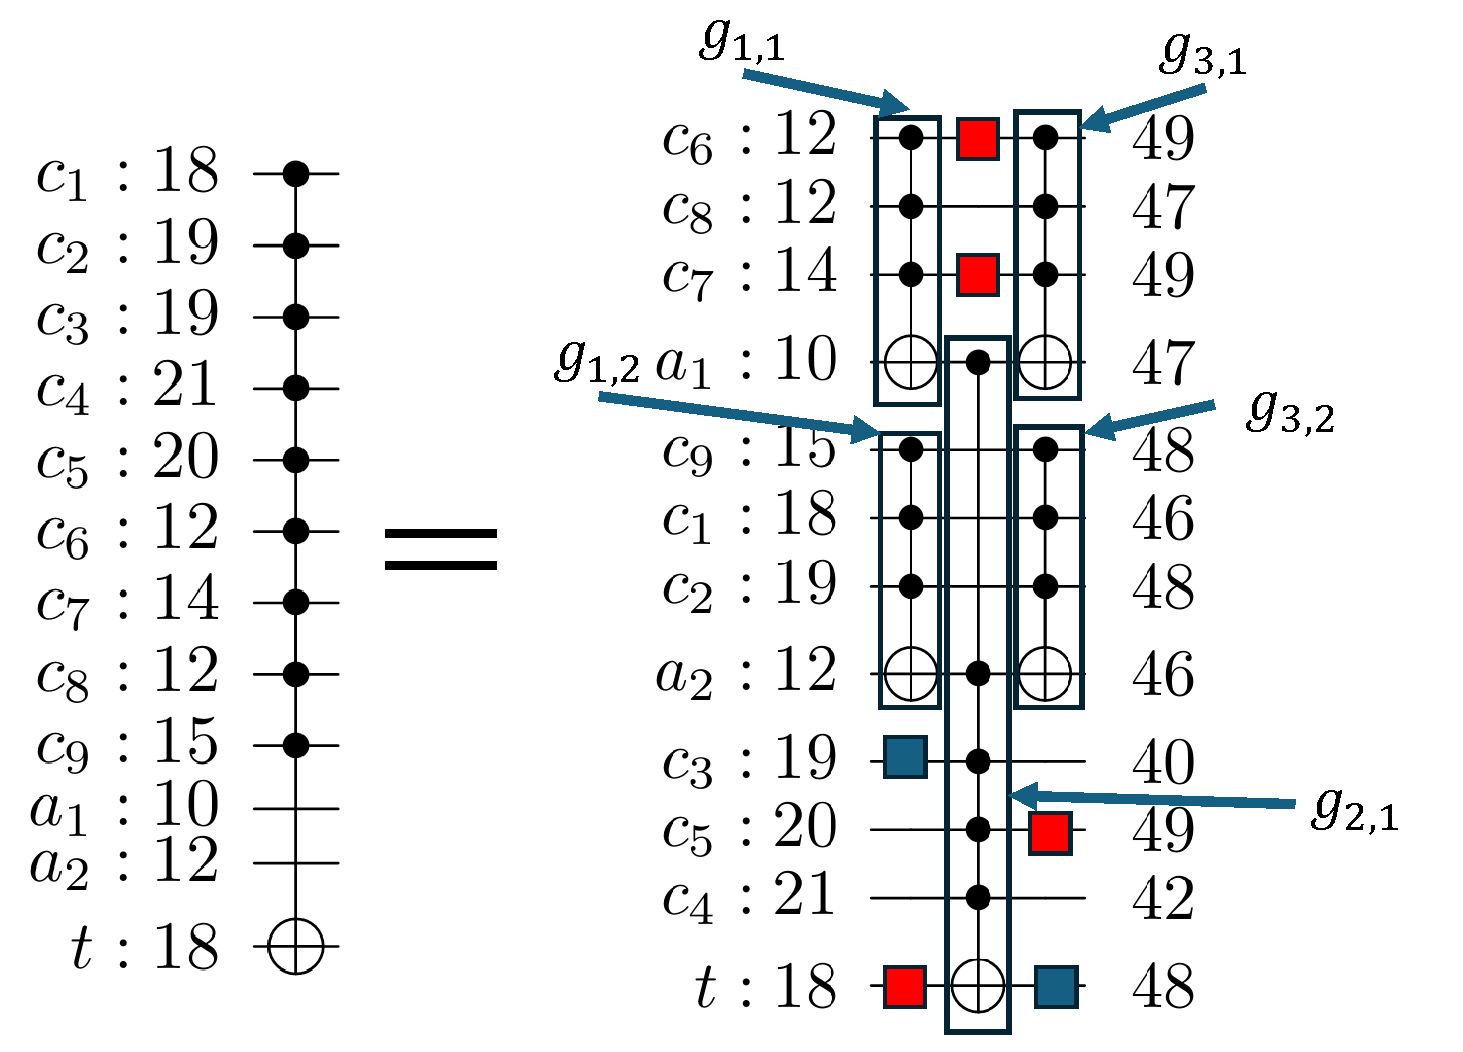
\includegraphics[width=10cm]{img/niemann_proposed.pdf}
  \caption{2個の値が0の補助ビットを用いて,ビットごとのT-depthを考慮し手法4を用いて,$c=9$のMCTゲートを分解した例}
  \label{niemann_proposed}
\end{figure}
\bout{図~\ref{niemann_proposed}に2個の値が0の補助ビットを用いて,
ビットごとのT-depthを考慮した手法~4で$c=9$のMCTゲートを分解した例を示す.
図~\ref{niemann_proposed}では,
分解前のMCTゲートのコントロールビットは$C=\{c_{1},\dots, c_{9}\}$となり,ターゲットビットは$t$である.
また,値が0の補助ビットは$CA=\{a_{1}, a_{2}\}$である.
まず,手法~4により各段のMCTゲートのコントロールビット数を求めると,式~\ref{eq:niemann_ctrl_gutairei}のようになる.
\begin{equation}\label{eq:niemann_ctrl_gutairei}
  \begin{pmatrix}
    3 & 3  \\
    5 &    \\
\end{pmatrix}
\end{equation}
この求めた数式~\ref{eq:niemann_ctrl_gutairei}のコントロールビット数に従い,各ゲートを構成するビットを決定する.
まず,1~段目のゲート$g_{1,1}, g_{1,2}$を構成するビットを決定する.
T-depthの小さい順にコントロールビットを$C$から選択すると,
1段目のゲートのコントロールビットは,それぞれ,$C_{1,1}=\{c_{6}, c_{8}, c_{7}\}$と,$C_{1,2}=\{c_{9}, c_{1}, c_{2}\}$となる.
選択したコントロールビットは$C$から削除する.
次に1段目のゲートのターゲットビットは,T-depthが小さい順に選択すると,それぞれ$a_{1}$, $a_{2}$となる.
選択した値が0の補助ビットは,$C$に追加し,$CA$から削除する.
1段目のゲート$g_{1,1},g_{1,2}$を構成するビットを決定した後,
$g_{1,1}, g_{1,2}$で使用していないビットの集合$A$を求める.
このとき,$A=\{c_{3}, c_{5}, c_{4}, t\}$となる.
このビットのうち,T-depthが小さい順に$c_{3},c_{5}$を補助ビットとして使用し,$g_{1,1}, g_{1,2}$を分解して,T-depthを更新する.
次に,2段目のゲート$g_{2,1}$を構成するビットを決定する.
2段目のゲートは中心のゲートであるため,
コントロールビットは残りの$C=\{a_{1},a_{2}, c_{3},c_{5}, c_{4}\}$となり,
ターゲットビットは$t$となる.
このようにして,$g_{1,1}, g_{1,2}, g_{2,1}$の構成するビットを決定する.
これらのゲートを構成するビットを決定した後,
式~\ref{eq:niemann_gates}の順でMCTゲートを配置すると,
図~\ref{niemann_proposed}の右側の分解となる.}
\par
\bout{最後に,図~\ref{niemann_proposed}の右側のゲートを
Algorithm~\ref{alg:method4_placement_decomp}に従い,分解する.
まず,1段目のゲート$g_{1,1}, g_{1,2}$を分解する.
$g_{1,1}$は赤色で塗りつぶされたビット$t$を補助ビットとして使用し分解する.
$g_{1,2}$は青色で塗りつぶされたビット$c_{3}$を補助ビットとして使用し分解する.
次に,$g_{1,1},g_{1,2}$の分解の結果から,
赤色で塗りつぶされたビット$c_{6},c_{7}$を補助ビットとして使用し,$g_{2,1}$を分解する.
最後に,$g_{2,1}$の分解の結果から,
$g_{3,1}, g_{3,2}$はそれぞれ,$c_{5}, t$を補助ビットとして使用し分解する.
このようにして,全てのゲートを分解すると,最大のT-depthは49となる.}
% どの補助ビットを選択したか図に書く.
\begin{comment}
提案手法では,
手法4により求めた各段のMCTゲートのコントロールビット数に従い,
分解後のMCTゲートの配置と分解を決定する.
Algorithm~\ref{}に各段のMCTゲートの配置,分解の決定方法を示す.
\begin{algorithm}[tbp]
  \caption{ビットごとのT-depthを考慮した手法~3の配置と分解}
  \label{alg:method3_placement_decomp}
  \begin{algorithmic}[1]
    \Require 分解前のMCTゲート$g=(C,t)$
    \Require 手法4で求めた各段のMCTゲートのコントロールビット数を表す2次元配列$CntList$
    \Require 値が0のビットのリスト$CA$
    \Require 値が不定のビットのリスト$DA$
    \Require 各ビットのT-depth
    \Ensure 分解後の回路$OC$
    \ForEach{$v$ in $CntList$}
    \State $n$:$v$の要素数
    \State $g_{1},\dots, g_{n}$:配置を行うMCTゲート
    \State $C_{1},\dots ,C_{n}$:各MCTゲートのコントロールビットの集合
    \State $t_{1},\dots ,t_{n}$:各MCTゲートのターゲットビット
    \ForEach{$c$ in $v$ with index $i$}
    \For{$j=1$ to $c$}
    \State $C_{i}$に$C$のT-depthが最も小さいビットを追加
    \State $C$からT-depthが最も小さいビットを削除
    \EndFor
    \State $t_{i}$に$CA$のT-depthが最も小さいビットを追加
    \State $CA$からT-depthが最も小さいビットを削除
    \EndFor
    \State $g_{1},\dots ,g_{n}$を同じ補助ビットを使わないよう,ビットごとのT-depthを考慮し分解
    \State $OC$に$g_{1},\dots g_{n}$の分解を追加
    \State T-depthを再計算
    \State $t_{1},\dots, t_{n}$を$C$に追加
    \EndFor
  \end{algorithmic}
\end{algorithm}
\end{comment}
\section{逆順での分解}
本節では,MCTゲートを逆順で分解する場合について説明する.
\begin{figure}[tbp]
  \centering
  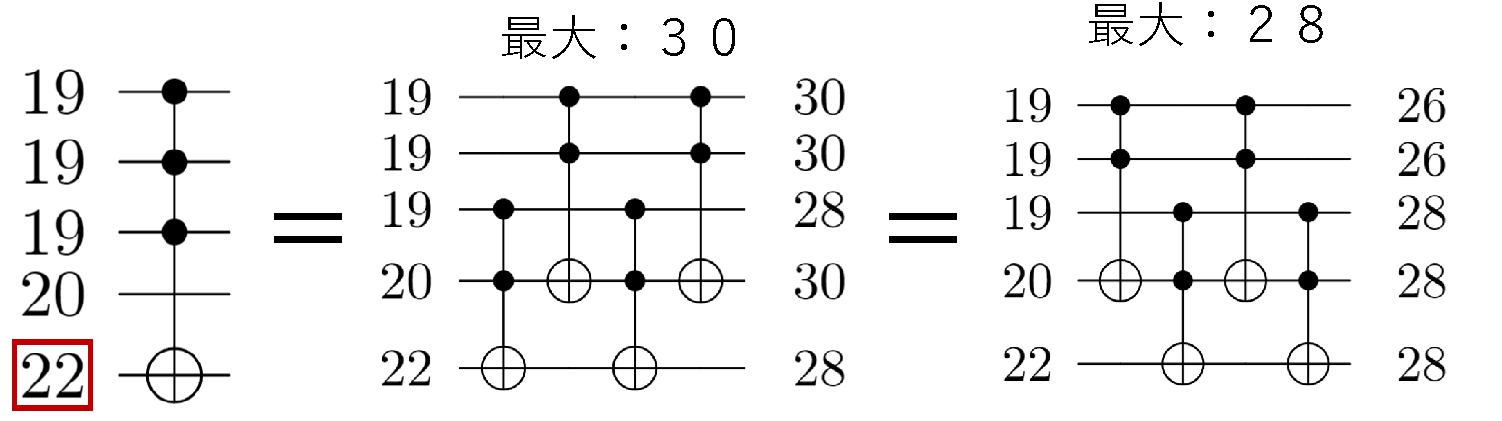
\includegraphics[width=10cm]{img/reverse_mct.pdf}
  \caption{コントロールビット数が3個のMCTゲートの分解とその逆順の分解}
  \label{reverse}
\end{figure}
\par
図~\ref{reverse}に示すように,
分解に使用する補助ビットと,分解するMCTゲートを構成するビットの中で,
ターゲットビットのT-depthが最も大きい場合,
MCTゲートを逆順で分解することで,
T-depthを削減できる.
図~\ref{reverse}の中心の分解は,
左側のMCTゲートを手法1の順で分解した場合を示している.
一方で右側の分解は,
左側のMCTゲートを手法1の分解と逆順に分解した場合を示している.
中心の例の分解では,
必ず最も左側のMCTゲートでターゲットビットを使用するため,
T-depthを削減することができない.
このため,
ターゲットビットのT-depthが最も大きい場合,逆順で分解することでT-depthを削減できる.
図~\ref{reverse}の例では,逆順でMCTゲートを分解することで最大のT-depthを2,削減している.
\par
手法1を用いて,MCTゲートを逆順で分解するには,
式~\ref{eq:toffoli_haiti}の逆順で配置する必要がある.
そのため,
$g_{2},\dots ,g_{c-1}, g_{1}$の順に優先的にT-depthが小さいビットを使用する必要がある.
分解前のMCTゲートの$c$個のコントロールビットを
T-depthが小さい順に並び変えたものを$c_{1},\dots, c_{c}$とする.
$g_{1},\dots, g_{c-1}$のコントロールビットの集合を$C_{1},\dots, C_{c-1}$とする.
$c-2$個の値が不定の補助ビットをT-depthの小さい順に並び変えたものを,$a_{1},\dots ,a_{c-2}$とする.
$g_{1},\dots ,g_{c-1}$の構成するビットの決定方法を以下に示す.
\begin{enumerate}[手順1]
  \item $g_{2}$のターゲットビットを$a_{1}$とする.
  \item $C_{2}\dots, C_{c-2}, C_{1}$に$a_{2},\dots, a_{c-2}, a_{1}$をそれぞれ順番に1つずつ追加する.
  \item $C_{2},\dots ,C_{c-2}$に順番に$c_{1},\dots ,c_{c-3}$を追加する.
  \item $C_{c-1}$に$c_{c-2}, c_{c-1}$を追加する.
  \item $C_{1}$に$c_{c}$と$a_{1}$を追加する.
  \item $g_{3},\dots, g_{c-2}$のターゲットビットをそれぞれ順番\rout{に}$a_{2}, \dots , a_{c-3}$とする.
  \item $g_{1}$のターゲットビットを$t$とする.
\end{enumerate}
$g_{1},\dots, g_{c-1}$の構成するビットを決定後,
式~\ref{eq:toffoli_haiti}の逆の順番で配置を行うことで,逆順で手法1の分解ができる.
\par
手法~2についても,逆順で分解することで,ターゲットビットを\bout{後で}使用できる.
配置する4つのMCTゲート$g_{1},\dots, g_{4}$と4つの$C\omega S$ゲートを逆順で配置することで,逆順の分解ができる.
分解に使用する1つの値が不定のビットを$a$とする.
4つの$C\omega S$ゲートは逆順で分解しても変わらず$a$をコントロールビットにもち,$t$をターゲットビットに持つ.
逆順で分解する場合$g_{4},\dots, g_{1}$の順で左側からMCTゲートを配置するため,
$g_{4}, g_{2}$にT-depthの小さいビットを配置する必要がある.
そのため,$g_{1}, g_{2}$のコントロールビットの集合を$C_{2}, C_{1}$として,
式~\ref{eq:method2bunkatu}の通りに$C_{1}, C_{2}$を決定する.
各ゲートを構成するビットを決定したら,
$g_{4}, C\omega S, g_{3}, C\omega S, \dots , g_{1}, C\omega S$の順で分解と配置を繰り返せば,
手法~2の逆順での分解を実現できる.
\par
手法3を逆順で分解するには,
式~\ref{eq:bakerhaiti}の逆順で分解したMCTゲートを配置する必要がある.
そのため,$g_{2},\dots, g_{m+1}, g_{1}$の順でT-depthの小さいビットを配置する必要がある.
分解に用いる$m$個の補助ビットの集合を$A$とする.
手法~3により求めた,
分解後の各MCTゲート$g_{1},\dots, g_{m+1}$の
コントロールビット数を$N_{1},\dots, N_{m+1}$とする.
$g_{1},\dots,g_{m+1}$のコントロールビットの集合を$C_{1},\dots, C_{m+1}$とする.
$g_{1},\dots,g_{m+1}$のターゲットビットを$t_{1},\dots, t_{m+1}$とする.
以下の手順に則り,$g_{1},\dots ,g_{m+1}$を構成するビットを決定する.
\begin{enumerate}[手順1]
  \item $g_{2}$を構成するビットを決定する.
  \begin{enumerate}
    \item $C_{2}$に$A$の最もT-depthが小さい要素を移動する.
    \item $t_{2}$に$A$の最もT-depthが小さい要素を移動する.
    \item $g_{2}$に$C$の最もT-depthが小さい要素を移動する.
  \end{enumerate}
  \item $g_{3},\dots, g_{m+1}$を構成するビットを決定する.
  \begin{enumerate}
    \item $i=3$とする.
    \item $C_{i}$に$A$から,T-depthが最小の要素を移動する.
    \item $|C_{i}|=N_{i}$となるよう,$C$からT-depthが小さい順に要素を移動する.
    \item $t_{i}$を$C_{i-1}$に移動した$A$の要素とする.
  \end{enumerate}
  \item $g_{1}$を構成するビットを決定する.
  \begin{enumerate}
    \item $C_{1}$に$t_{2}$を加える.
    \item $C_{1}$に,$C$の残りの要素を移動する.
    \item $t_{1}$を$t$とする.
  \end{enumerate}
 \end{enumerate}
 このような手順で$g_{1},\dots ,g_{m+1}$を構成するビットを決定し,式~\ref{eq:bakerhaiti}の逆の順でゲートを配置,
 分解することで,手法3についても逆順で分解できる.
 \par
 手法4については,分解が左右対称であるため,逆順で分解してもT-depthに変化がない.
% 手法2,3個別に説明をいれる.
\section{\bout{後続}のゲートを考慮した\bout{ビームサーチによる分解手法}}
後続のゲートを考慮し,\bout{ビームサーチによってMCTゲートの分解を行う手法を説明する.}
\par
図~\ref{select_ancilla_tdepth}に,
2つのMCTゲート$g_{1}, g_{2}$の補助ビットの選択によるT-depthの変化を示す.
図~\ref{select_ancilla_tdepth}の\bout{真ん中}の例は,
$g_{1}$が赤で塗りつぶされたT-depth最小の補助ビットを選択し分解,
$g_{2}$が$g_{1}$の分解の結果を受けて,青で塗りつぶされたT-depth最小のビットを選択し,分解した例である.
図~\ref{select_ancilla_tdepth}の右側の例では,
$g_{1}$が赤で塗りつぶされたT-depthが41の補助ビットを選択し,分解,
$g_{2}$が$g_{1}$の分解の結果を受けて,
青で塗りつぶされた,T-depth最小のビットを選択した例である.
図~\ref{select_ancilla_tdepth}中心の例では,
最大のT-depthが58となるのに対し,
右側の例では,最大のT-depthが53となる.
\begin{figure}[tbp]
  \centering
  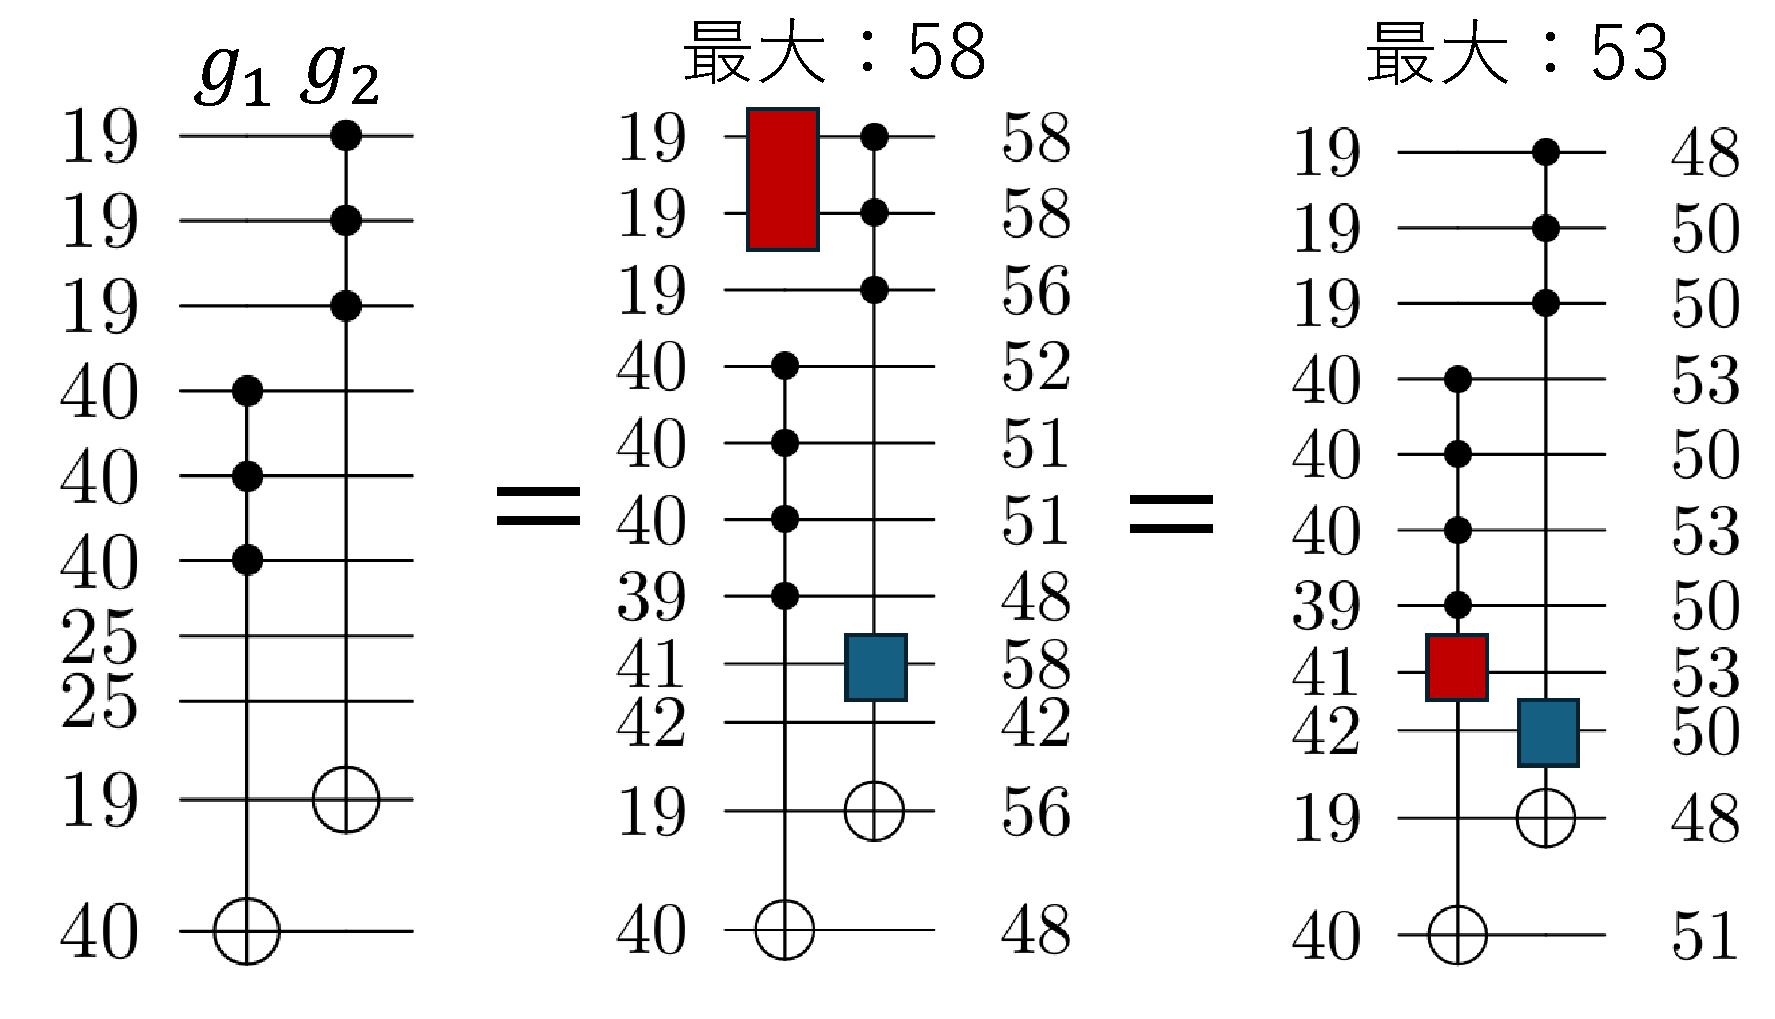
\includegraphics[width=10cm]{img/select_ancilla_biit_tdepth.pdf}
  \caption{2つのMCTゲートの補助ビットの選択によるT-depthの変化の例}
  \label{select_ancilla_tdepth}
\end{figure}
図~\ref{bad_consider_tdepth}の中心の例のように,
貪欲にT-depthの小さいビットを選択した場合,
\bout{後続}のゲートを分解した場合にT-depthが悪化する場合がある.
このため,分解するゲートの\bout{後続}のゲートを考慮しMCTゲートを分解することが必要である.
\par
ビットごとのT-depthを考慮したMCTゲートの分解を行う場合,
MCTゲートの分解の結果に応じて各ビットのT-depthが変化する.
そこで,各ノードの評価値をT-depthの最大値とし,
各MCTゲートの分解を遷移とし,木を構成する.
この木を全探索することで,最適な分解を求めることができる.
しかし,全探索を行うと量子ビット数と,
分解を行うMCTゲート数が増加すると計算量が膨大になる.
このため,ビームサーチ\cite{bisiani1992beam}を用い,
探索範囲を事前に決めておいた数の候補に限定することで,
現実的な計算量に抑えて,探索を行う.
\par
ここで,各MCTゲートの分解の列挙も制限する.
すべての分解を列挙するには,すべての補助ビットの選択の組み合わせを列挙しなければならない.
コントロールビット数が$c$のMCTゲートは,$1$から$c-2$個の値が不定の補助ビットを選択できる.
使用できる値が不定の補助ビットの数が$m$とすると,
値が不定の補助ビットの選び方は,$\sum_{i = 1}^{c-2} {}_mC_{i}$通りとなる.
回路の量子ビット数と回路を構成するMCTゲートのコントロールビット数が増加すると,
補助ビットの選択をすべて列挙することは難しいため,
規定した分解を遷移として,遷移の数を制限する.
規定した分解は次の通りである.
\begin{enumerate}[(1)]
  \item T-depthが小さい順に1から$c-2$個の値が不定の補助ビットを選択
  \item T-depthが小さい順に1から$c-2$個の値が0の補助ビットを選択
  \item 分解を行うゲートの一つ後のゲートが使用していないビットを,値が不定のビットとして,T-depthが小さい順に1から$c-2$個選択する.
  \item これらの分解の逆順の分解
\end{enumerate}
\par
MCTゲートの分解を遷移とし,分解を行った後のT-depthの最大値を評価値として,
ビームサーチを行う疑似コードをAlgorithm~\ref{alg:mct_beam}に示す.
図~\ref{mct_beam}に,
図~\ref{select_ancilla_tdepth}の$g_{1}$の分解を
Algorithm~\ref{alg:mct_beam}に従い,
決定する様子を示す.
図~\ref{mct_beam}の探索する幅は3,探索する深さは2とする.
また,簡単のため,逆順の分解については列挙しない.
まず,図~\ref{mct_beam}では,
$g_{1}$の分解\rout{$D_{1},\dots, D_{4}$を列挙する.}
分解$D_{1},\dots,D_{4}$から求まる回路の最大のT-depthをノードの評価値とする.
評価値の小さい順にノードをソートし,
上位3つのノードから,次のゲート$g_{2}$の分解を列挙する.
$g_{2}$の分解の結果からT-depthを計算し,
評価値が最小のノードの最初の遷移を$g_{1}$の分解として決定する.
この例では,$D_{3}$が$g_{1}$の分解として決定する.
\begin{figure}[tbp]
  \centering
  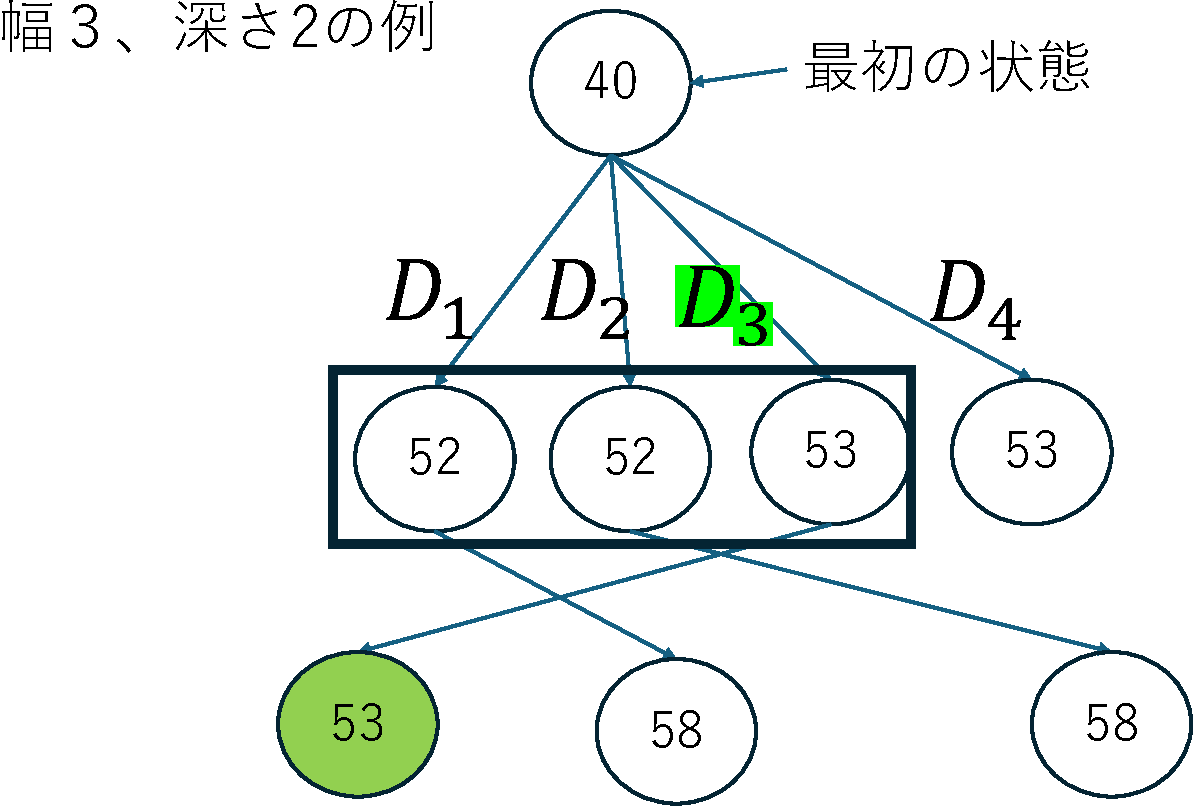
\includegraphics[width=8cm]{img/mct_beam.pdf}
  \caption{図~\ref{select_ancilla_tdepth}の$g_{1}$の分解をAlgorithm~\ref{alg:mct_beam}に従い決定するようす}
  \label{mct_beam}
\end{figure}
提案手法では,MCTゲートで構成される回路に対して,1ゲートずつ,
Algrorithm~\ref{alg:mct_beam}に基づいて分解を決定していき,すべてのゲートを分解する.
% 具体例を付けるべきか,図の例だと大した例にならない.
\begin{comment}
図~\ref{mct_beam}に探索する深さ2,幅3でビームサーチを用いて,
図~\ref{bad_consider_tdepth}を後のゲートを考慮しMCTゲートの分解を決定する様子を示す.
\begin{figure}[tbp]
  \centering
  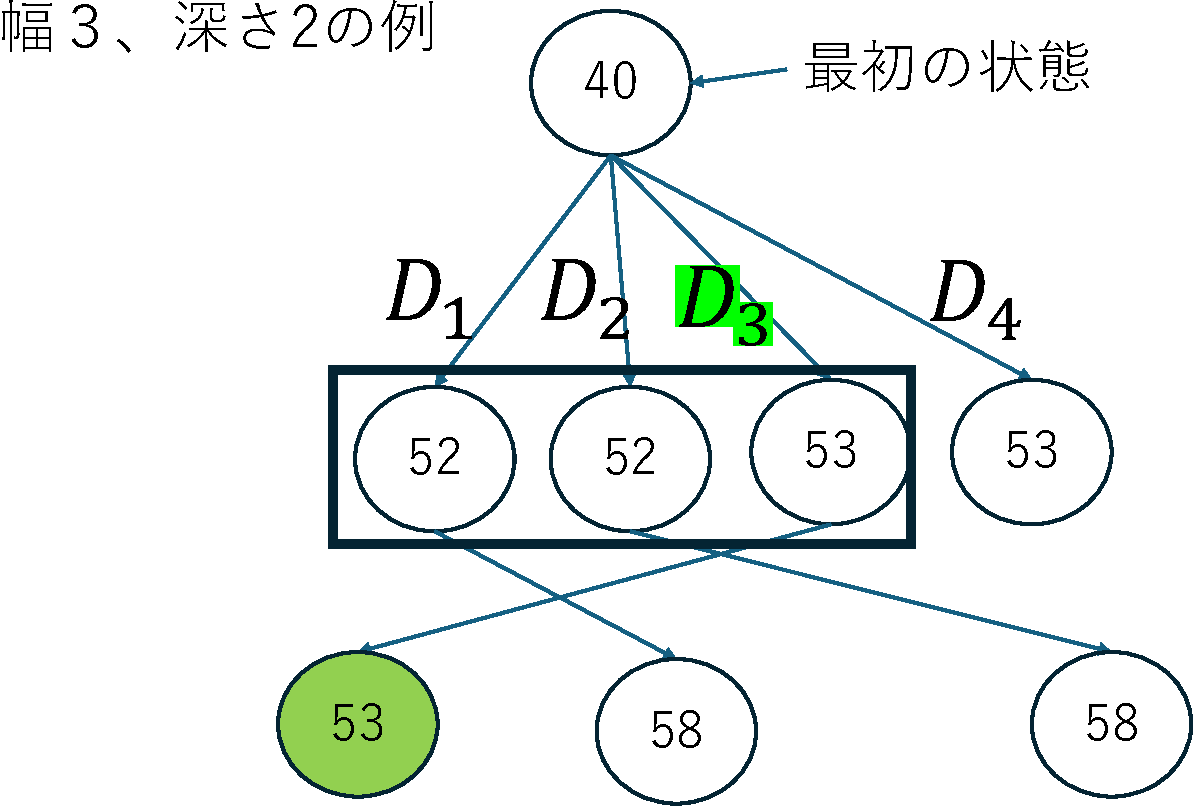
\includegraphics[width=10cm]{img/mct_beam.pdf}
  \caption{2つのMCTゲートの補助ビットの選択によるT-depthの変化の例}
  \label{mct_beam}
\end{figure}
\end{comment}

\begin{algorithm}[tbp]
  \caption{T-depthの最大値を評価値とするビームサーチの疑似コード}
  \label{alg:mct_beam}
  \begin{algorithmic}[1]
    \Require $state$:(T-depthの最大値,ビットごとのT-depth,分解を行うMCTゲート)
    \Require $legal\_actions$:MCTゲートの分解を列挙し,次のゲート分解前の状態を返す関数
    \Require $depth$:探索する深さ
    \Require $width$:探索する幅
    \State $best\_decomp$:最良の候補
    \State $candidate\_list$ 探索候補のリスト,優先度付きキュー
    \State $candidate\_list.push(state)$
    \For{$1,..,depth$}
      \State $next\_candidate\_list$ 次の探索候補のリスト,優先度付きキュー
      \For{$1,..,width$}
      \If{$candidate\_list$が空なら}
        \State break
      \EndIf
      \State $now\_state \Leftarrow candidate\_list.pop()$ 探索候補の最良の値を取り出し,popする
      \State $next\_candidate\_list.push(legal\_actions(now\_state))$ 次の探索候補のリストに現在の状態からの遷移を追加
      \EndFor
      \State $candidate\_list \Leftarrow next\_candidate\_list$ 探索候補のリストを更新
      \State $best\_decomp \Leftarrow candidate\_list.top()$ 最良の候補を更新
    \EndFor
    \State \Return $best\_decomp$の最初の遷移を返す
  \end{algorithmic}
\end{algorithm}

\chapter{実験結果と考察}
本章では,実験結果と考察について述べる.
\section{実験方法}
\begin{table}[tbp]
  \centering
  \caption{実験に用いた計算環境}
  \label{tab:env}
  \begin{tabular}{l|l}
      \hline
      CPU & AMD Ryzen 9 7950X3D 16-Core Processor \\
      RAM & 128GB    \\
      OS  & \rout{Ubuntu 22.04.03 LTS}    \\ \hline
  \end{tabular}
\end{table}
\begin{table}[tbp]
  \centering
  \caption{実験を行ったRevLibベンチマーク回路}
  \label{tab:revlib}
  \begin{tabular}{l|r|r|r}
      \hline
      ベンチマーク回路名& 量子ゲート数 & 量子ビット数 & 最大コントロールビット数 \\ \hline
      9symml\_195 & 129 & 10 & 9    \\
      add6\_196   & 229 & 19 & 7      \\
      adr4\_197   & 55 & 13 & 5      \\
      alu2\_199   & 157 & 16 & 10      \\
      alu3\_200   & 94 & 18 & 10      \\
      alu\_319    & 15764 & 235 & 36  \\
      apla\_200   & 80 & 22 & 9      \\
      clip\_206   & 174 & 14 & 9      \\
      cm85a\_209  & 69 & 14 & 7      \\
      cordic\_218 & 2533 & 25 & 17   \\
      dc2\_222    & 75 & 15 & 7        \\
      decod\_217  & 80 & 21 & 5      \\
      f51m\_233   & 663 & 22 & 14      \\
      ham15\_107  & 132 & 15 & 7      \\
      misex3c\_244& 1721 & 28 & 14 \\
      sqrt8\_260  & 40 & 12 & 7      \\
      sym10\_262  & 194 & 11 & 10    \\
      sym9\_148   & 210 & 10 & 4      \\
      tial\_265   & 1041 & 22 & 12     \\ \hline
  \end{tabular}
\end{table}
提案手法の評価を行うために,
既存手法と提案手法をRustで実装し,比較実験を行った.
実験に用いた,計算環境は表~\ref{tab:env}の通りである.
MCTゲートで構成される,
RevLib~\cite{wille2008revlib}のベンチマーク回路に,補助ビットを追加し,
第3章で説明した既存手法の分解を適用した回路,
第4章で説明した提案手法の分解を適用した回路の最大のT-depthをそれぞれ比較した.
使用したRevLibベンチマーク回路の一覧を表~\ref{tab:revlib}に示す.
\section{実験結果}
値が不定の補助ビットを表~\ref{tab:revlib}の回路に
1,3,5,10個\bout{追加し},実験を行った結果をそれぞれ表~\ref{tab:d_1_result}~\ref{tab:d_10_result}に示す.
また,値が0の補助ビットを表~\ref{tab:revlib}の回路に
1,3,5,10個\bout{追加し},実験を行った結果をそれぞれ表~\ref{tab:k_1_result}~\ref{tab:k_10_result}に示す.
\par
表中の既存(1)は,
既存手法1~4のうち,
最大のT-depthが最も小さくなる分解を各ゲートに適用した場合の,
回路全体の最大のT-depthを表す.
表中の提案(2)は,
補助ビットをビットのT-depthが小さい順に選択し,
最大のT-depthが最も小さくなる提案手法の分解を
各ゲートに適用した場合の,
回路全体の最大のT-depthを表す.
表中の提案(3)は,
Algorithm~\ref{alg:mct_beam}に基づき,
探索する幅10,探索する深さ10で,
各ゲートの分解を決定した場合の,
回路全体の最大のT-depthを表す.
表中の削減率は,
提案(3)と既存(1)を比較した場合の,
最大のT-depthの削減率を表す.
割合が正の場合,既存(1)に対して,
提案(3)の最大のT-depthが減少している.
\par
表~\ref{tab:d_1_result}~\ref{tab:d_10_result}のすべての場合で,削減率が正となっている.
実験を行ったすべての回路で提案手法は最大のT-depthを削減できた.
表~\ref{tab:d_1_result}~\ref{tab:d_10_result}の提案(3)の平均のT-depth削減率はそれぞれ,20.98%,21.71%,22.54%,23.7%である.
1種類の回路を除き,
全ての場合で提案(3)の方が提案(2)よりも小さい最大のT-depthとなっている.
\par
表~\ref{tab:k_1_result}~\ref{tab:k_10_result}のすべての場合で,削減率が正となっている.
実験を行ったすべての回路で提案手法は最大のT-depthを削減できた.
表~\ref{tab:k_1_result}~\ref{tab:k_10_result}の提案(3)の平均のT-depth削減率はそれぞれ,13.71%,11.94%,13.05%,8.97%である.
1種類の回路を除き,
全ての場合で提案(3)の方が提案(2)よりも小さい最大のT-depthとなっている.
\section{考察}
値が不定の補助ビットを回路に\bout{追加した}場合は,
\bout{追加した}補助ビットの数が増加するほど,
提案手法の平均のT-depth削減率が増加する.
これは,追加の補助ビットにより,
分解に使用できる補助ビットの数が増加したことで,
T-depthの小さいビットを補助ビットとして,
多くの分解で使用できるようになったためと考えられる.
\par
値が0の補助ビットを回路に\bout{追加した}場合は,
与えた補助ビットの数が増加するほど,
平均のT-depth削減率が減少する傾向にある.
\rout{値が0の補助ビットが,
分解するMCTゲートのコントロールビット数-2個存在すると,
図~\ref{niemann_c_2}のようにToffoliゲートを並列に配置し,MCTゲートを分解できる.}
この分解では,ビットごとのT-depthはほとんど差が生じない.
\rout{このため,}値が0の補助ビットが増加した結果,
多くのMCTゲートの分解結果が図~\ref{niemann_c_2}の分解となり,
提案手法を適用しても既存手法から,
大きく最大のT-depthを削減できなかったと考えられる.
\par
回路に\bout{追加した}補助ビット数が増加するほど,
提案(3)の計算時間は増加する傾向にある.
これは,分解に使用できる補助ビット数が増加すると,
Algorithm~\ref{alg:mct_beam}中で列挙する分解が増加し,
1ゲートの分解を決定する時間が増加するためであると考えられる.
\begin{table}[tbp]
  \centering
  \caption{表~\ref{tab:revlib}の回路に1個の値が不定の補助ビットを\bout{追加した}場合の実験結果}
  \label{tab:d_1_result}
  \begin{tabular}{l|r|r|r|r|r}
      \hline
      {\footnotesize ベンチマーク名} &{\footnotesize \begin{tabular}{c} 既存(1)\\(ベスト)\end{tabular} } & {\footnotesize \begin{tabular}{c} 提案(2)\\(貪欲)\end{tabular}} & {\footnotesize \begin{tabular}{c} 提案(3)\\(ビームサーチ)\end{tabular}} & {\footnotesize \begin{tabular}{c} 提案(3)\\ 削減率(%)\end{tabular}}& {\footnotesize \begin{tabular}{c} 提案(3)\\ 計算時間(秒)\end{tabular}} \\ \hline
      9symml\_195                    &2202                      &1990                       &1966                       &10.72                               &8.616463849        \\
      add6\_196                      &2647                      &2008                       &1941                       &26.67                               &18.31790732        \\
      adr4\_197                      &327                       &264                        &255                        &22.02                               &0.399761523        \\
      alu2\_199                      &1874                      &1519                       &1469                       &21.61                               &15.3711949         \\
      alu3\_200                      &1027                      &845                        &775                        &24.54                               &8.081885731        \\
      alu\_319                       &698553                    &537044                     &530175                     &24.1                                &16846.8836         \\
      apla\_200                      &1352                      &1087                       &1027                       &24.04                               &12.00728189        \\
      clip\_206                      &2176                      &1897                       &1785                       &17.97                               &12.00482561        \\
      cm85a\_209                     &900                       &688                        &682                        &24.22                               &6.464221294        \\
      cordic\_218                    &85744                     &77817                      &72315                      &15.66                               &565.2734203        \\
      dc2\_222                       &794                       &638                        &609                        &23.3                                &2.283650357        \\
      decod\_217                     &805                       &656                        &616                        &23.48                               &6.493433718        \\
      f51m\_233                      &11708                     &9545                       &9146                       &21.88                               &80.43032866        \\
      ham15\_107                     &852                       &701                        &681                        &20.07                               &3.635737611        \\
      misex3c\_244                   &41995                     &34889                      &31978                      &23.85                               &285.5496817        \\
      sqrt8\_260                     &252                       &205                        &202                        &19.84                               &0.339.63529        \\
      sym10\_262                     &3876                      &3464                       &3463                       &10.66                               &14.94273904        \\
      sym9\_148                      &2168                      &1731                       &1700                       &21.59                               &6.153590018        \\
      tial\_265                      &19614                     &15785                      &15222                      &22.39                               &95.84991401        \\ \hline
  \end{tabular}
\end{table}

\begin{table}[tbp]
  \centering
  \caption{表~\ref{tab:revlib}の回路に3個の値が不定の補助ビットを\bout{追加した}場合の実験結果}
  \label{tab:d_3_result}
  \begin{tabular}{l|r|r|r|r|r}
      \hline
      {\footnotesize ベンチマーク名} &{\footnotesize \begin{tabular}{c} 既存(1)\\(ベスト)\end{tabular} } & {\footnotesize \begin{tabular}{c} 提案(2)\\(貪欲)\end{tabular}} & {\footnotesize \begin{tabular}{c} 提案(3)\\(ビームサーチ)\end{tabular}} & {\footnotesize \begin{tabular}{c} 提案(3)\\ 削減率(%)\end{tabular}}& {\footnotesize \begin{tabular}{c} 提案(3)\\ 計算時間(秒)\end{tabular}} \\ \hline
      9symml\_195                    &1837                      &1655                       &1646                       & 10.4                               &7.629649027                            \\
      add6\_196                      &2647                      &2007                       &1934                       & 26.94                              &18.58197403                            \\
      adr4\_197                      &327                       &261                        &249                        & 23.85                              &0.465260219                            \\
      alu2\_199                      &1862                      &1458                       &1415                       & 24.01                              &9.969310544                            \\
      alu3\_200                      &1027                      &828                        &781                        & 23.95                              &11.36386762                            \\
      alu\_319                       &698553                    &536923                     &530175                     & 24.1                               &17090.14273                            \\
      apla\_200                      &1352                      &1070                       &1030                       & 23.82                              &16.62229704                            \\
      clip\_206                      &2148                      &1815                       &1678                       & 21.88                              &12.86709908                            \\
      cm85a\_209                     &900                       &698                        &678                        & 24.67                              &9.785195934                            \\
      cordic\_218                    &82160                     &74961                      &67966                      & 17.28                              &611.8083509                            \\
      dc2\_222                       &794                       &648                        &619                        & 22.04                              &7.630411817                            \\
      decod\_217                     &805                       &656                        &616                        & 23.48                              &6.493433718                            \\
      f51m\_233                      &11630                     &9328                       &8906                       & 23.42                              &57.74939339                            \\
      ham15\_107                     &852                       &691                        &683                        & 19.84                              &6.391189206                            \\
      misex3c\_244                   &41995                     &34572                      &32049                      & 23.68                              &278.5653425                            \\
      sqrt8\_260                     &252                       &206                        &195                        & 22.62                              &1.199307345                            \\
      sym10\_262                     &3282                      &2923                       &2929                       & 10.76                              &14.73540026                            \\
      sym9\_148                      &2168                      &1745                       &1692                       & 21.96                              &12.56517508                            \\
      tial\_265                      &19614                     &15613                      &14943                      & 23.81                              &94.95900956                            \\ \hline
  \end{tabular}
\end{table}

\begin{table}[tbp]
  \centering
  \caption{表~\ref{tab:revlib}の回路に5個の値が不定の補助ビットを\bout{追加した}場合の実験結果}
  \label{tab:d_5_result}
  \begin{tabular}{l|r|r|r|r|r}
      \hline
      {\footnotesize ベンチマーク名} &{\footnotesize \begin{tabular}{c} 既存(1)\\(ベスト)\end{tabular} } & {\footnotesize \begin{tabular}{c} 提案(2)\\(貪欲)\end{tabular}} & {\footnotesize \begin{tabular}{c} 提案(3)\\(ビームサーチ)\end{tabular}} & {\footnotesize \begin{tabular}{c} 提案(3)\\ 削減率(%)\end{tabular}}& {\footnotesize \begin{tabular}{c} 提案(3)\\ 計算時間(秒)\end{tabular}} \\ \hline
      9symml\_195                    &1618                      &1378                       &1374                       &15.08                               &9.930336017                           \\
      add6\_196                      &2647                      &2012                       &1923                       &27.35                               &18.01739652                           \\
      adr4\_197                      &327                       &264                        &251                        &23.24                               &0.714814204                           \\
      alu2\_199                      &1862                      &1434                       &1398                       &24.92                               &12.0442911                           \\
      alu3\_200                      &1027                      &799                        &769                        &25.12                               &7.776029939                           \\
      alu\_319                       &698553                    &537020                     &530114                     &24.11                               &17037.31845                           \\
      apla\_200                      &1352                      &1051                       &1021                       &24.48                               &11.33025049                           \\
      clip\_206                      &2148                      &1782                       &1671                       &22.21                               &12.34393723                           \\
      cm85a\_209                     &900                       &680                        &681                        &24.33                               &10.22069656                           \\
      cordic\_218                    &79600                     &73066                      &64712                      &18.7                                &615.7103987                           \\
      dc2\_222                       &794                       &635                        &605                        &23.8                                &4.908101386                           \\
      decod\_217                     &805                       &630                        &617                        &23.35                               &6.611246125                           \\
      f51m\_233                      &11610                     &9219                       &8812                       &24.1                                &83.74010086                           \\
      ham15\_107                     &852                       &695                        &686                        &19.48                               &6.122892557                           \\
      misex3c\_244                   &41995                     &34401                      &32003                      &23.79                               &293.6476532                           \\
      sqrt8\_260                     &252                       &203                        &194                        &23.02                               &1.1009005                           \\
      sym10\_262                     &2906                      &2477                       &2456                       &15.49                               &16.96328378                           \\
      sym9\_148                      &2168                      &1735                       &1692                       &21.96                               &10.0843481                           \\
      tial\_265                      &19614                     &15459                      &14948                      &23.79                               &116.83510061                           \\ \hline
  \end{tabular}
\end{table}


\begin{table}[tbp]
  \centering
  \caption{表~\ref{tab:revlib}の回路に10個の値が不定の補助ビットを\bout{追加した}場合の実験結果}
  \label{tab:d_10_result}
  \begin{tabular}{l|r|r|r|r|r}
      \hline
      {\footnotesize ベンチマーク名} &{\footnotesize \begin{tabular}{c} 既存(1)\\(ベスト)\end{tabular} } & {\footnotesize \begin{tabular}{c} 提案(2)\\(貪欲)\end{tabular}} & {\footnotesize \begin{tabular}{c} 提案(3)\\(ビームサーチ)\end{tabular}} & {\footnotesize \begin{tabular}{c} 提案(3)\\ 削減率(%)\end{tabular}}& {\footnotesize \begin{tabular}{c} 提案(3)\\ 計算時間(秒)\end{tabular}} \\ \hline
      9symml\_195                    &1585                      &1242                       &1235                       &22.08                               &12.98424072                            \\
      add6\_196                      &2647                      &1952                       &1919                       &27.5                                &10.78927272                            \\
      adr4\_197                      &327                       &267                        &257                        &21.41                               &0.865038196                            \\
      alu2\_199                      &1862                      &1395                       &1376                       &26.1                                &11.46544858                            \\
      alu3\_200                      &1027                      &781                        &773                        &24.73                               &11.86293436                            \\
      alu\_319                       &698553                    &537544                     &530031                     &24.12                               &17004.74323                            \\
      apla\_200                      &1352                      &1069                       &1014                       &25                                  &16.76269416                            \\
      clip\_206                      &2148                      &1715                       &1637                       &23.79                               &15.79988978                            \\
      cm85a\_209                     &900                       &663                        &656                        &27.11                               &9.435726005                            \\
      cordic\_218                    &78576                     &68487                      &61059                      &22.29                               &639.2620752                            \\
      dc2\_222                       &794                       &609                        &601                        &24.31                               &4.161026199                            \\
      decod\_217                     &805                       &633                        &616                        &23.48                               &5.066818825                            \\
      f51m\_233                      &11610                     &8942                       &8700                       &25.06                               &88.38343134                            \\
      ham15\_107                     &852                       &700                        &681                        &20.07                               &7.17699178                             \\
      misex3c\_244                   &41995                     &33772                      &31967                      &23.88                               &291.8650831                            \\
      sqrt8\_260                     &252                       &206                        &199                        &21.03                               &968.386954                             \\
      sym10\_262                     &2747                      &2168                       &2148                       &21.81                               &21.96572075                            \\
      sym9\_148                      &2168                      &1752                       &1688                       &22.14                               &13.51507038                            \\
      tial\_265                      &19614                     &15376                      &14844                      &24.32                               &94.64945337                            \\ \hline
      \end{tabular}
\end{table}

\begin{table}[tbp]
  \centering
  \caption{表~\ref{tab:revlib}の回路に1個の値が0の補助ビットを\bout{追加した}場合の実験結果}
  \label{tab:k_1_result}
  \begin{tabular}{l|r|r|r|r|r}
      \hline
      {\footnotesize ベンチマーク名} &{\footnotesize \begin{tabular}{c} 既存(1)\\(ベスト)\end{tabular} } & {\footnotesize \begin{tabular}{c} 提案(2)\\(貪欲)\end{tabular}} & {\footnotesize \begin{tabular}{c} 提案(3)\\(ビームサーチ)\end{tabular}} & {\footnotesize \begin{tabular}{c} 提案(3)\\ 削減率(%)\end{tabular}}& {\footnotesize \begin{tabular}{c} 提案(3)\\ 計算時間(秒)\end{tabular}} \\ \hline
      9symml\_195                    &1876                      &1824                       &1639                       &12.63                               &5.354373132                             \\
      add6\_196                      &2125                      &1876                       &1807                       &14.96                               &24.83758234                             \\
      adr4\_197                      &273                       &240                        &237                        &13.19                               &1.333745029                             \\
      alu2\_199                      &1543                      &1402                       &1359                       &11.92                               &18.43510636                             \\
      alu3\_200                      &834                       &769                        &726                        &12.95                               &12.42137057                             \\
      alu\_319                       &638401                    &526555                     &520941                     &18.4                                &22853.74644                             \\
      apla\_200                      &1122                      &1009                       &969                        &13.64                               &18.61791974                             \\
      clip\_206                      &1769                      &1711                       &1631                       &7.8                                 &20.51546752                             \\
      cm85a\_209                     &718                       &643                        &634                        &11.7                                &9.560854838                             \\
      cordic\_218                    &82828                     &65211                      &63359                      &23.51                               &714.7813002                             \\
      dc2\_222                       &637                       &595                        &583                        &8.48                                &8.580471124                             \\
      decod\_217                     &668                       &619                        &604                        &9.58                                &6.019526017                             \\
      f51m\_233                      &10218                     &8865                       &8537                       &16.45                               &82.49771624                             \\
      ham15\_107                     &716                       &644                        &641                        &10.47                               &5.861906917                             \\
      misex3c\_244                   &37130                     &32373                      &31036                      &16.41                               &408.9865322                             \\
      sqrt8\_260                     &206                       &193                        &184                        &10.68                               &0.605509814                             \\
      sym10\_262                     &3491                      &3086                       &2966                       &15.04                               &14.37715293                             \\
      sym9\_148                      &1842                      &1585                       &1540                       &16.4                                &13.72147056                             \\
      tial\_265                      &17236                     &14806                      &14422                      &16.33                               &139.1230812                             \\ \hline
  \end{tabular}
\end{table}

\begin{table}[tbp]
  \centering
  \caption{表~\ref{tab:revlib}の回路に3個の値が0の補助ビットを\bout{追加した}場合の実験結果}
  \label{tab:k_3_result}
  \begin{tabular}{l|r|r|r|r|r}
      \hline
      {\footnotesize ベンチマーク名} &{\footnotesize \begin{tabular}{c} 既存(1)\\(ベスト)\end{tabular} } & {\footnotesize \begin{tabular}{c} 提案(2)\\(貪欲)\end{tabular}} & {\footnotesize \begin{tabular}{c} 提案(3)\\(ビームサーチ)\end{tabular}} & {\footnotesize \begin{tabular}{c} 提案(3)\\ 削減率(%)\end{tabular}}& {\footnotesize \begin{tabular}{c} 提案(3)\\ 計算時間(秒)\end{tabular}} \\ \hline
      9symml\_195                    &1107                      &1024                       &994                        &10.21                               &10.35821939           \\
      add6\_196                      &1633                      &1512                       &1442                       &11.7                                &32.71605484           \\
      adr4\_197                      &232                       &216                        &210                        &9.48                                &2.500321032           \\
      alu2\_199                      &1207                      &1095                       &1059                       &12.26                               &25.80267911           \\
      alu3\_200                      &647                       &611                        &575                        &11.13                               &17.79894466           \\
      alu\_319                       &492490                    &385249                     &384624                     &21.9                                &33086.71708           \\
      apla\_200                      &835                       &802                        &737                        &11.74                               &7.473599686           \\
      clip\_206                      &1316                      &1265                       &1201                       &8.74                                &25.35615578           \\
      cm85a\_209                     &534                       &503                        &488                        &8.61                                &15.61660338           \\
      cordic\_218                    &56426                     &50521                      &48458                      &14.12                               &1126.454378           \\
      dc2\_222                       &503                       &469                        &453                        &9.94                                &11.80918567           \\
      decod\_217                     &540                       &524                        &511                        &5.37                                &9.874927362           \\
      f51m\_233                      &8459                      &7086                       &6844                       &19.09                               &123.5022412           \\
      ham15\_107                     &595                       &563                        &563                        &5.38                                &8.1572118             \\
      misex3c\_244                   &31058                     &25847                      &25130                      &19.09                               &584.7197648           \\
      sqrt8\_260                     &167                       &155                        &149                        &10.78                               &1.876260938           \\
      sym10\_262                     &1997                      &1825                       &1746                       &12.57                               &22.11154212           \\
      sym9\_148                      &1470                      &1365                       &1395                       &5.1                                 &17.91198214           \\
      tial\_265                      &14589                     &12011                      &11728                      &19.61                               &227.8126735           \\ \hline
  \end{tabular}
\end{table}

\begin{table}[tbp]
  \centering
  \caption{表~\ref{tab:revlib}の回路に5個の値が0の補助ビットを\bout{追加した}場合の実験結果}
  \label{tab:k_5_result}
  \begin{tabular}{l|r|r|r|r|r}
      \hline
      {\footnotesize ベンチマーク名} &{\footnotesize \begin{tabular}{c} 既存(1)\\(ベスト)\end{tabular} } & {\footnotesize \begin{tabular}{c} 提案(2)\\(貪欲)\end{tabular}} & {\footnotesize \begin{tabular}{c} 提案(3)\\(ビームサーチ)\end{tabular}} & {\footnotesize \begin{tabular}{c} 提案(3)\\ 削減率(%)\end{tabular}}& {\footnotesize \begin{tabular}{c} 提案(3)\\ 計算時間(秒)\end{tabular}} \\ \hline
      9symml\_195                    &811                       &791                        &779                        &3.95                                &15.1548317              \\
      add6\_196                      &1516                      &1377                       &1348                       &11.08                               &37.89277818              \\
      adr4\_197                      &232                       &214                        &210                        &9.48                                &1.658355848              \\
      alu2\_199                      &1003                      &932                        &908                        &9.47                                &29.3668285              \\
      alu3\_200                      &574                       &537                        &511                        &10.98                               &21.09317769              \\
      alu\_319                       &392027                    &263224                     &258874                     &33.97                               &44371.48937              \\
      apla\_200                      &717                       &681                        &669                        &6.69                                &31.83563098              \\
      clip\_206                      &1133                      &1080                       &1061                       &6.35                                &32.93731216              \\
      cm85a\_209                     &485                       &449                        &446                        &8.04                                &17.3571338              \\
      cordic\_218                    &46438                     &27113                      &26760                      &42.37                               &1561.342406              \\
      dc2\_222                       &474                       &447                        &436                        &8.02                                &16.26663139              \\
      decod\_217                     &540                       &524                        &511                        &5.37                                &10.77430374              \\
      f51m\_233                      &6313                      &4995                       &4882                       &22.67                               &160.8829675              \\
      ham15\_107                     &590                       &556                        &556                        &5.76                                &8.612412013              \\
      misex3c\_244                   &22340                     &18209                      &17589                      &21.27                               &808.0919446              \\
      sqrt8\_260                     &162                       &148                        &146                        &9.88                                &1.763942013              \\
      sym10\_262                     &1436                      &1362                       &1341                       &6.62                                &24.40247407              \\
      sym9\_148                      &1470                      &1365                       &1392                       &5.31                                &16.1889075              \\
      tial\_265                      &10382                     &8463                       &8238                       &20.65                               &276.7313876              \\ \hline
  \end{tabular}
\end{table}

\begin{table}[tbp]
  \centering
  \caption{表~\ref{tab:revlib}の回路に10個の値が0の補助ビットを\bout{追加した}場合の実験結果}
  \label{tab:k_10_result}
  \begin{tabular}{l|r|r|r|r|r}
      \hline
      {\footnotesize ベンチマーク名} &{\footnotesize \begin{tabular}{c} 既存(1)\\(ベスト)\end{tabular} } & {\footnotesize \begin{tabular}{c} 提案(2)\\(貪欲)\end{tabular}} & {\footnotesize \begin{tabular}{c} 提案(3)\\(ビームサーチ)\end{tabular}} & {\footnotesize \begin{tabular}{c} 提案(3)\\ 削減率(%)\end{tabular}}& {\footnotesize \begin{tabular}{c} 提案(3)\\ 計算時間(秒)\end{tabular}} \\ \hline
      9symml\_195                    &728                       &712                        &712                        &2.2                                 &13.50758898                            \\
      add6\_196                      &1516                      &1367                       &1342                       &11.48                               &37.45163841                            \\
      adr4\_197                      &232                       &213                        &210                        &9.48                                &1.308176433                            \\
      alu2\_199                      &938                       &870                        &861                        &8.21                                &32.3252184                             \\
      alu3\_200                      &555                       &513                        &500                        &9.91                                &24.37575513                            \\
      alu\_319                       &327158                    &225315                     &221960                     &32.16                               &63609.29504                       \\
      apla\_200                      &668                       &641                        &634                        &5.09                                &36.31744878                            \\
      clip\_206                      &1081                      &1031                       &1018                       &5.83                                &32.17092475                            \\
      cm85a\_209                     &485                       &444                        &443                        &8.66                                &19.47420972                            \\
      cordic\_218                    &29752                     &23805                      &23304                      &21.67                               &485.8965619                            \\
      dc2\_222                       &474                       &447                        &435                        &8.23                                &15.64473569                            \\
      decod\_217                     &540                       &524                        &511                        &5.37                                &8.806832537                            \\
      f51m\_233                      &4811                      &4369                       &4341                       &9.77                                &236.5839665                            \\
      ham15\_107                     &588                       &556                        &556                        &5.44                                &10.20320188                            \\
      misex3c\_244                   &16687                     &15496                      &15440                      &7.47                                &1138.943443                            \\
      sqrt8\_260                     &162                       &148                        &146                        &9.88                                &2.451909686                            \\
      sym10\_262                     &1235                      &1185                       &1185                       &4.05                                &27.86129776                            \\
      sym9\_148                      &1470                      &1361                       &1390                       &5.44                                &17.76674975                            \\
      tial\_265                      &7936                      &7268                       &7265                       &8.46                                &449.0854821                            \\ \hline 
  \end{tabular}
\end{table}
\chapter{おわりに}
本論文では,
ビットごとのT-depthを考慮して,
MCTゲートを分解することで,
量子回路全体の最大のT-depthを削減する手法を提案した.
既存手法のMCTゲートの分解では,
ビットごとのT-depthを考慮していないため,
量子回路全体のT-depthが増加する場合が\rout{ある}.
提案手法では,ビットごとのT-depthを考慮して,
T-depthの小さなビットを優先して使用し,
MCTゲートを分解することで,
T-depthを削減\rout{できる}.
また,後続のゲートを考慮して,
ビームサーチを用いてMCTゲートを分解することで,
回路全体のT-depthを削減する手法を提案した.
ベンチマーク回路を用いて,
既存手法,提案手法それぞれを適用した回路の最大のT-depthを比較した.
\par
\rout{実験を行った}すべての回路で提案手法は既存手法よりも,最大のT-depthを削減でき,
\rout{最大のT-depthを平均17.1%}削減できることを確認した.
また,後続のゲートを考慮しビームサーチを用いて,
MCTゲートを分解することで,
計算時間は増加するがより多くのT-depthが削減できることを確認した.
\par
ビットごとのT-depthを考慮した,
手法2\rout{から}手法4の分解では,
MCTゲートをコントロールビット数の少ないMCTゲートに分解し,
再帰的にMCTゲートを分解する.
提案手法では,
このコントロールビット数の少ないMCTゲートを構成するビットを決定する際に,
T-depthの小さいビットを優先して配置している.
\rout{その際},
これらのMCTゲートを再帰的に分解するための補助ビットを考慮していない.
今後の課題としては,
手法2\rout{から}手法4において,より最大のT-depthを小さくするような,
各MCTゲートを構成するビットの決定方法を検討することが考えられる.
また,後続のゲートを考慮し,
ビームサーチを用いて分解を決定する手法では,
最大のT-depthが小さい分解が多く存在する場合,
局所解に陥り,
最大のT-depthが改善されない場合が考えられる.
そのため,
列挙する分解を確率的に選択することで,
より良い解を探索する手法の検討も今後の課題として考えられる.
 \begin{comment} 
 \begin{itemize}
   \item 得られた成果
   \item 結論
   \item 課題
     \begin{itemize}
       \item 再帰的に分解する場合にT-depth最小となる分解
       \item ビームサーチの改善
     \end{itemize}
\end{itemize}
\end{comment} 
\input{7-acknowledgement}

\bibliographystyle{junsrt}
\bibliography{ref}
\end{document}
